%%%%%%%%%%%%%%%%%%%%%%%%%%%%%%%%%%%%%%%%%%%%%%%%%%%%%%%%%%%%%%%%%%%%%%%%%%%%%%%
%                                                                             %
% VARIATIONAL MONTE CARLO METHODS FOR QUANTUM DOTS, by Matteo Seclì           %
%                                                                             %
% This eBook is meant to be used as the BSc Thesis of the author.             %
% The predicted date of the discussion is 22/07/2015 at the University of     %
% Trento.                                                                     %
%                                                                             %
% For licensing information, look at the LICENSE file shipped with this       %
% document.                                                                   %
%                                                                             %
% The original location of this project is at                                 %
% https://github.com/matteosecli/QMC.                                         %
%                                                                             %
% Title: Variational Monte Carlo Methods for quantum dots                     %
%                                                                             %
% Author: Matteo Seclì <secli.matteo@gmail.com>                               %
%                                                                             %
% Language: English                                                           %
%                                                                             %
% Character set encoding: UTF-8                                               %
%                                                                             %
% *** START OF THIS BACHELOR THESIS PROJECT ***                               %
%                                                                             %
%%%%%%%%%%%%%%%%%%%%%%%%%%%%%%%%%%%%%%%%%%%%%%%%%%%%%%%%%%%%%%%%%%%%%%%%%%%%%%%


%%%%%%%%%%%%%%%%%%%%%%%%%%%%%%%%%%%%%%%%%%%%%%%%%%%%%%%%%%%
% Basic class definitions, typesetting, bibliography      %
%%%%%%%%%%%%%%%%%%%%%%%%%%%%%%%%%%%%%%%%%%%%%%%%%%%%%%%%%%%
\documentclass[a4paper,twoside,11pt]{book}
\usepackage[utf8]{inputenc}
\usepackage{type1cm}
\usepackage{setspace}
\usepackage[english]{babel}
\usepackage{datetime}
\usepackage[sort, round]{natbib}


%%%%%%%%%%%%%%%%%%%%%%%%%%%%%%%%%%%%%%%%%%%%%%%%%%%%%%%%%%%
% Hyperref configuration                                  %
%%%%%%%%%%%%%%%%%%%%%%%%%%%%%%%%%%%%%%%%%%%%%%%%%%%%%%%%%%%
\usepackage[%hypertex,
	unicode=true,
	plainpages = false, 
	pdfpagelabels, 
	bookmarks=true,
	bookmarksnumbered=true,
    bookmarksopen=true,
	breaklinks=true,
	backref=false,
	colorlinks=true,
	linkcolor = blue,		% Use "blue" if you want to highlight them
	urlcolor  = blue,
	citecolor = red,
	anchorcolor = green,
	hyperindex = true,
	linktocpage = true,
	hyperfigures
]{hyperref}


%%%%%%%%%%%%%%%%%%%%%%%%%%%%%%%%%%%%%%%%%%%%%%%%%%%%%%%%%%%
% Grahpics                                                %
%%%%%%%%%%%%%%%%%%%%%%%%%%%%%%%%%%%%%%%%%%%%%%%%%%%%%%%%%%%
\usepackage{graphicx}
\usepackage{xcolor}
\graphicspath{{figures/PNG/}{figures/PDF/}{figures/}}
\usepackage{tikz}
\usepackage[siunitx]{circuitikz}


%%%%%%%%%%%%%%%%%%%%%%%%%%%%%%%%%%%%%%%%%%%%%%%%%%%%%%%%%%%
% Standard environments                                   %
%%%%%%%%%%%%%%%%%%%%%%%%%%%%%%%%%%%%%%%%%%%%%%%%%%%%%%%%%%%
\usepackage{float}
\usepackage[font={small,it}]{caption}[2013/01/06] % Minimum version required for incompatibility with breqn
\usepackage{subcaption}
\usepackage{listingsutf8}
\usepackage{enumitem}


%%%%%%%%%%%%%%%%%%%%%%%%%%%%%%%%%%%%%%%%%%%%%%%%%%%%%%%%%%%
% Math                                                    %
%%%%%%%%%%%%%%%%%%%%%%%%%%%%%%%%%%%%%%%%%%%%%%%%%%%%%%%%%%%
\usepackage{amsmath}
\usepackage{amssymb}	
\usepackage{amsthm}
\usepackage{cancel}
\usepackage{braket}
\usepackage{siunitx}
\DeclareSIUnit\atomicunit{a.u.}
\usepackage{breqn}
\usepackage{geometry}
\renewenvironment{proof}{\vskip 1em \noindent\textsc{Proof:}}{\begin{flushright}$\blacksquare$\end{flushright}\vskip 1em}


%%%%%%%%%%%%%%%%%%%%%%%%%%%%%%%%%%%%%%%%%%%%%%%%%%%%%%%%%%%
% datetime specific configuration                         %
%%%%%%%%%%%%%%%%%%%%%%%%%%%%%%%%%%%%%%%%%%%%%%%%%%%%%%%%%%%
\newdateformat{monthyear}{\monthname[\THEMONTH] \THEYEAR}


%%%%%%%%%%%%%%%%%%%%%%%%%%%%%%%%%%%%%%%%%%%%%%%%%%%%%%%%%%%
% TikZ specific configuration                             %
%%%%%%%%%%%%%%%%%%%%%%%%%%%%%%%%%%%%%%%%%%%%%%%%%%%%%%%%%%%
\usetikzlibrary{shapes.geometric, arrows, patterns}
\tikzstyle{startstop} = [rectangle, rounded corners, minimum width=3cm, minimum height=1cm,text centered, draw=black, fill=red!30]
\tikzstyle{io} = [trapezium, trapezium left angle=70, trapezium right angle=110, minimum width=3cm, minimum height=1cm, text centered, draw=black, fill=blue!30]
\tikzstyle{process} = [rectangle, minimum width=3cm, minimum height=1cm, text centered, text width=3cm, draw=black, fill=orange!30]
\tikzstyle{decision} = [diamond, minimum width=3cm, minimum height=1cm, text centered, draw=black, fill=green!30]
\tikzstyle{arrow} = [thick,->,>=stealth]


%%%%%%%%%%%%%%%%%%%%%%%%%%%%%%%%%%%%%%%%%%%%%%%%%%%%%%%%%%%
% xcolor specific configuration                           %
%%%%%%%%%%%%%%%%%%%%%%%%%%%%%%%%%%%%%%%%%%%%%%%%%%%%%%%%%%%
\definecolor{dkgreen}{rgb}{0,0.6,0}
\definecolor{dred}{rgb}{0.545,0,0}
\definecolor{dblue}{rgb}{0,0,0.545}
\definecolor{lgrey}{rgb}{0.9,0.9,0.9}
\definecolor{gray}{rgb}{0.4,0.4,0.4}
\definecolor{darkblue}{rgb}{0.0,0.0,0.6}


%%%%%%%%%%%%%%%%%%%%%%%%%%%%%%%%%%%%%%%%%%%%%%%%%%%%%%%%%%%
% ListingsUTF8 specific configuration                     %
%%%%%%%%%%%%%%%%%%%%%%%%%%%%%%%%%%%%%%%%%%%%%%%%%%%%%%%%%%%
\lstdefinelanguage{cpp}{
	backgroundcolor=\color{lgrey},  
	basicstyle=\footnotesize \ttfamily \color{black} \bfseries,   
	breakatwhitespace=false,       
	breaklines=true,               
	captionpos=b,                   
	commentstyle=\color{dkgreen},   
	deletekeywords={...},          
	escapeinside={\%*}{*)},                  
	frame=single,                  
	language=C++,                
	keywordstyle=\color{purple},  
	morekeywords={BRIEFDescriptorConfig,string,TiXmlNode,DetectorDescriptorConfigContainer,
		istringstream,cerr,exit}, 
	identifierstyle=\color{black},
	stringstyle=\color{blue},      
	numbers=right,                 
	numbersep=5pt,                  
	numberstyle=\tiny\color{black}, 
	rulecolor=\color{black},        
	showspaces=false,               
	showstringspaces=false,        
	showtabs=false,                
	stepnumber=1,                   
	tabsize=5,                     
	title=\lstname,                 
}


%%%%%%%%%%%%%%%%%%%%%%%%%%%%%%%%%%%%%%%%%%%%%%%%%%%%%%%%%%%
% Some black magic                                        %
%%%%%%%%%%%%%%%%%%%%%%%%%%%%%%%%%%%%%%%%%%%%%%%%%%%%%%%%%%%
\makeatletter
	\renewcommand{\bibsection}{\chapter{\bibname}}
\makeatother


%%%%%%%%%%%%%%%%%%%%%%%%%%%%%%%%%%%%%%%%%%%%%%%%%%%%%%%%%%%
% Metadata                                                %
%%%%%%%%%%%%%%%%%%%%%%%%%%%%%%%%%%%%%%%%%%%%%%%%%%%%%%%%%%%
\def\THauthor{Matteo Seclì}
\def\THsupervisor{Morten Hjorth-Jensen, UiO}
\def\THextrasupervisor{Francesco Pederiva, UniTN}
\def\THtitle{Variational Monte Carlo methods for quantum dots} % title
\def\THdate{\monthyear\today}
\def\THplace{Trento}
\title{\THtitle}
\author{\THauthor}


%%%%%%%%%%%%%%%%%%%%%%%%%%%%%%%%%%%%%%%%%%%%%%%%%%%%%%%%%%%
% Actual text                                             %
%%%%%%%%%%%%%%%%%%%%%%%%%%%%%%%%%%%%%%%%%%%%%%%%%%%%%%%%%%%

\begin{document}

\frontmatter
%\maketitle

\graphicspath{{Frontmatter/figures/PNG/}{Frontmatter/figures/PDF/}{Frontmatter/figures/}}

\begin{titlepage}
	\newgeometry{margin=3.5cm}
	
	\begin{center}
	
		
\includegraphics[width=10cm]{logo-unitn-dphys}\\[0.4cm]
		
		\vskip 5.5cm
		
		{\Large Degree in Physics}\\[0.5cm]
		
		{\Large Thesis}\\[0.5cm]
		
		% Title
		\rule{\linewidth}{0.2mm} \\[0.5cm]
		
		{ \huge \bfseries \THtitle \\[0.5cm] }
		
		\rule{\linewidth}{0.2mm} \\[2cm]
		
		% Author and supervisor
		\begin{minipage}[t]{0.45\textwidth}
			\begin{flushleft} \large
				\emph{Supervisors:} \\[0.25cm]
				Prof. \THsupervisor \\[0.10cm]
				Prof. \THextrasupervisor
			\end{flushleft}
		\end{minipage}
		\begin{minipage}[t]{0.45\textwidth}
			\begin{flushright} \large
				\emph{Student:}\\[0.25cm]
				{ \THauthor }
			\end{flushright}
		\end{minipage}
		
		\vfill
		
		% Bottom of the page
		{\large A.Y. 2014/2015}
		
	\end{center}
	
	\restoregeometry
\end{titlepage}
\onehalfspacing	% Set 1.5 lines spacing for better readability
%%%%%%%%%%%%%%%%%%%%%%%%%%%%%%%%%%%%%%%%%%%%%%%%%%%%%%%%%%%
%                                                         %
% PREFACE                                                 %
%                                                         %
% This file is part of a BSc Thesis Project. See the      %
% LICENSE file for more information about licensing.      %
%                                                         %
% Author:     Matteo Seclì <secli.matteo@gmail.com>       %
% A.Y.:       2014/2015                                   %
% URL:        https://github.com/matteosecli/QMC          %
%                                                         %
%%%%%%%%%%%%%%%%%%%%%%%%%%%%%%%%%%%%%%%%%%%%%%%%%%%%%%%%%%%

\chapter{Preface}

Here I am, finally, writing this very last project after three years at the University of Trento.

This work has a strong computational taste, but my interest in computing and programming is quite an old story. I still remember that, as a child, I spent a lot of time learning the DOS 6 and how to program in Pascal and JavaScript. This interest has grown over the years and it eventually led me to discover new languages and new problems to solve. I've developed my own projects about the most different varieties of subjects: from basic cryptography to audio/video streams, to web-based platforms, to more scientific challenges with Matlab or Mathematica.

Until one year ago, I had no chance to blend this passion with the primary interest of my life: Physics. But then I've been offered a one-year exchange program at the University of Oslo, and I immediately chose ``Computational Physics'' as an optional class. The course exceeded my best expectations, mainly thanks to the professor, Morten Hjorth-Jensen, who did a great job in passing on his passion to his students. I've always spoken freely to him about those sides of Physics I like the most: the state-of-the-art mathematical formulations, the fundamental laws, and the quantum world -- as soon as I discovered it in the ``Quantum Mechanics'' course at the University of Oslo. In particular the latter had a great impact on my life, since I decided to follow the ``quantum path'' for my coming master studies.

Since professor Morten Hjorth-Jensen was well aware of my interests and I asked his guide for a more complex project, he proposed me a project tailored on my passions: a simulation of quantum dots, developed via Monte Carlo methods. The project immediately draw my entire attention and I spent almost two months at programming and analyzing the results, trying to shape my simulator in a more extensible way that allows to run it even on different systems (e.g., atoms). Later I further extended the project with the help of professor Francesco Pederiva, who suggested me some additional reading material that gave me better insights about the world of quantum dots.

This thesis is the result of these months of work. I went through many difficulties; non-working code, endless obscure ``segmentation fault'' errors, negative values for the kinetic energy (clearly, some sort black magic happening in the code), programming nights at the university (``because the night is dark and full of coffee''), and days spent trying to figure out the meaning of very bad-written articles. Not to speak about the parallelization, because I had a hard time trying to separate completely all the different threads.

In the end I survived this jungle, but it would haven't been possible without the help of many people that I want to thank. First of all I want to say a big thank to professor Morten Hjorth-Jensen, that inspired me so much that I've decided to take a quantum-oriented master course in Computational Physics. I also want to thank Jørgen Høgberget, that helped me a lot with the code and made my days happier by saying around random Italian words like ``mozzarella'' and ``gorgonzola'' with a terrible and funny accent. Last but not least, I want to thank all of my friends, my family and my grandparents, that supported me during these years even with hard sacrifices. A big thank also goes to all of my professors both at the University of Trento and at the University of Oslo, that helped and guided me up to this point. Thank you all!

\begin{flushright}
	{ \THauthor }
\end{flushright}
\begin{flushleft}
	{ \THplace, \THdate }
\end{flushleft}



%%%%%%%%%%%%%%%%%%%%%%%%%%%%%%%%%%%%%%%%%%%%%%%%%%%%%%%%%%%
%                                                         %
% INTRODUCTION                                            %
%                                                         %
% This file is part of a BSc Thesis Project. See the      %
% LICENSE file for more information about licensing.      %
%                                                         %
% Author:     Matteo Seclì <secli.matteo@gmail.com>       %
% A.Y.:       2014/2015                                   %
% URL:        https://github.com/matteosecli/QMC          %
%                                                         %
%%%%%%%%%%%%%%%%%%%%%%%%%%%%%%%%%%%%%%%%%%%%%%%%%%%%%%%%%%%

\chapter{Introduction}

The aim of this work is to introduce the use of the Variational Monte Carlo (VMC) method in the analysis of physical systems. In particular, we focus here on quantum dots with $N = 2$ and $N = 6$ electrons.

The first chapter contains a brief introduction about these devices, giving insights about construction methods and physical modeling. The discussion proceeds by introducing a first model, called the \emph{shell-model}, that explains why we have a better stability for certain numbers of electrons and justifies the fact that we are restricting our discussion to quantum dot systems of only $N = 2$ and $N = 6$ electrons (and possibly $12, 20, \ldots$). These particular systems are called the \emph{closed-shell systems}.

Then, a model called the \emph{Coulomb blockade model} is introduced in order to explain characteristic oscillations in conductance measurements. The model is explained both in an intuitive and in a more systematical way.

At the end of the first chapter we show some results derived from both experiments and theoretical and numerical calculations, that justify the fact the potential inside our quantum dots is commonly shaped as a two-dimensional harmonic oscillator.

The second chapter is dedicated to quantum mechanical considerations about the electron system and we introduce the variational principle and the Metropolis algorithm, both in its brute-force sampling and importance sampling variants. 

The third and the fourth chapters show the calculation results for the $N=2$ and the $N=6$ systems, respectively. We will begin with two electrons confined in a pure two-dimensional isotropic harmonic potential, with and without the repulsive interaction, developing a simple trial wave-function and a basic program that runs our calculations. Then we are going to improve the trial wave-function adding the so-called \emph{Jastrow factor}, and finally we are going to extend the entire class of wave-functions and the program itself to a given number of electrons (those corresponding to closed-shell systems). After that we are going to improve our sampling, switching from a brute-force approach to the clever \emph{importance sampling}.

Chapter five presents a brief analysis of our results in comparison with the virial theorem, while in chapter six we develop a first attempt at improving the code. This is done by exploiting the mathematical properties of the trial wave-function and the diffusive quantum-force, in order to simplify the calculation of the derivatives.

\tableofcontents

\mainmatter
%%%%%%%%%%%%%%%%%%%%%%%%%%%%%%%%%%%%%%%%%%%%%%%%%%%%%%%%%%%
%                                                         %
% CHAPTER 01:                                             %
% What are quantum dots?                                  %
%                                                         %
% This file is part of a BSc Thesis Project. See the      %
% LICENSE file for more information about licensing.      %
%                                                         %
% Author:     Matteo Seclì <secli.matteo@gmail.com>       %
% A.Y.:       2014/2015                                   %
% URL:        https://github.com/matteosecli/QMC          %
%                                                         %
%%%%%%%%%%%%%%%%%%%%%%%%%%%%%%%%%%%%%%%%%%%%%%%%%%%%%%%%%%%

\graphicspath{{Mainmatter/figures/PNG/}{Mainmatter/figures/PDF/}{Mainmatter/figures/}}

\chapter{What are quantum dots?}

\section{Definition and fabrication processes}
The term ``quantum dots'' refers to finite fermion systems consisting of an artificial 3D confinement of a few electrons, that have a size of only a few hundred angstroms \citep{Reimann2002, Kastner1993}.

Such confinement is usually achieved by restricting the two-dimensional electron gas that forms at the interface between two different semiconductor materials (or heterostructure), ether laterally or vertically. Let's briefly examine these two methods.

\begin{figure}[H]
	\centering
	\begin{subfigure}[t]{0.5\textwidth}
		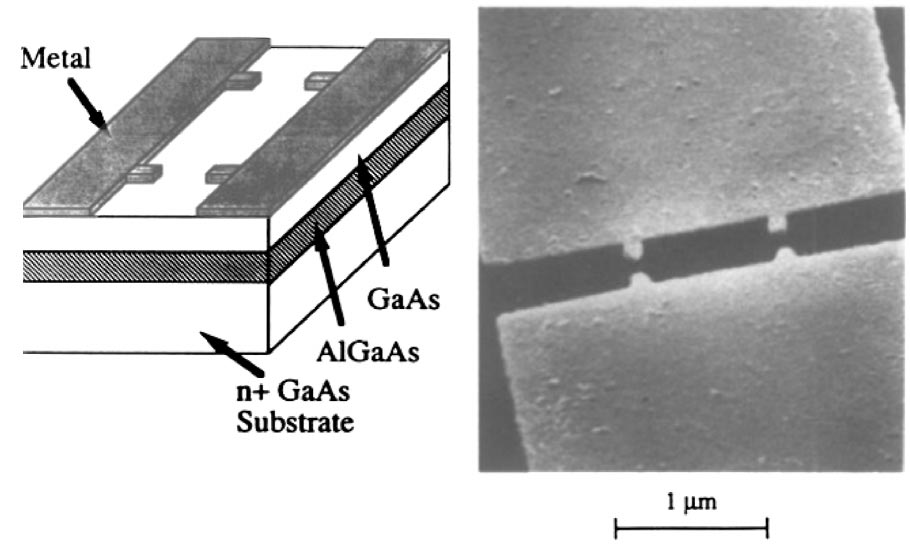
\includegraphics[width=\textwidth]{Figure_5_Reimann}
		\caption{Lateral device structure. From \cite{Meirav1990}.}
		\label{fig:Figure_5_Reimann}
    \end{subfigure}
	\begin{subfigure}[t]{0.4\textwidth}
		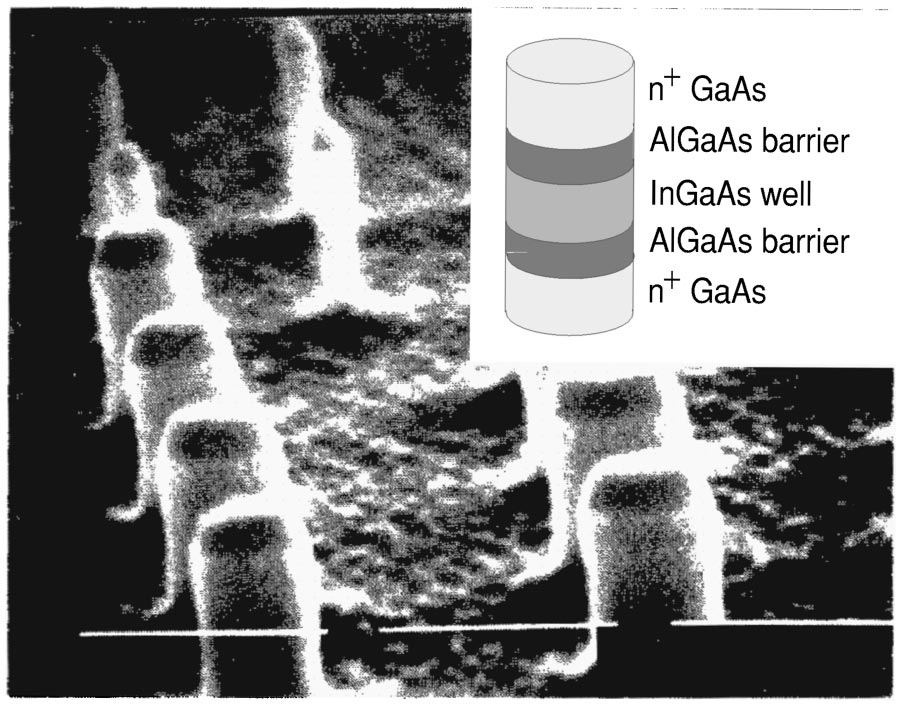
\includegraphics[width=\textwidth]{Figure_4_Reimann}
		\caption{Etched quantum dots. The white bars have a length of $\SI{0.5}{\micro\meter}$. From \cite{Reed1988}.}
		\label{fig:Figure_4_Reimann}
    \end{subfigure}
    \caption{Lateral and vertical quantum dots structures.}
	\label{fig:Figures_4-5_Reimann}
\end{figure}

The lateral confinement is obtained with a device like the one in Figure \ref{fig:Figure_5_Reimann}. The electron gas forms at the interface between GaAs and AlGaAs, and the confinement is obtained by applying a voltage to the top metal electrodes -- called gates. The entire structure is only a few $\SI{}{\micro\meter}$ thick, so the gates are created by lithographic patterning.

Another common method to fabricate quantum dots is to build heterostructure pillars by etching techniques. Some of these structures are shown in Figure \ref{fig:Figure_4_Reimann} the electrodes are at the top and at the bottom of the pillars.

Other fabricating processes include self-growth mechanisms, in which the growth conditions determine the form of the structure (that can be pyramidal, disk shaped or lens shaped), and cleaved-edge overgrowth, that consists in two separate MBE\footnote{Molecular Beam Epitaxy} growths on a specific substrate \citep[see][]{Reimann2002}.

Although the definition of quantum dots given above is quite precise, I prefer a more immediate one: ``quantum dots are \emph{artificial atoms}''. Despite its simplicity, this definition contains a good amount of relevant information. Like natural atoms, in fact, quantum dots are made up of electrons confined in an attractive potential; and as one may guess, they show a similar shell-like structure with its relative \emph{magic numbers} -- the resemblance is striking. We begin our discussion by briefly illustrating this simple model.

\section{The shell-model}
\label{sec:shell_model}
The so-called \emph{shell-model} is a particularly convenient and simple way to treat a system of interacting particles. This model is based on the \emph{a priori} assumption that the \emph{interacting} particles can be treated as \emph{independent} particles subject to an average \emph{effective potential}. This effective potential is created by the particles themselves, but one can also add an external component to the intrinsic one. Using this simplification it's possible to find a solution for the Schr\"{o}dinger equation; the result is a certain distribution of single-particle energy levels. In many cases, this distribution it's nonuniform (look, for example, at the simple case of the infinite well) and shows a characteristic bunching of levels; these bunches are called \emph{shells}.

\begin{figure}[H]
	\centering
    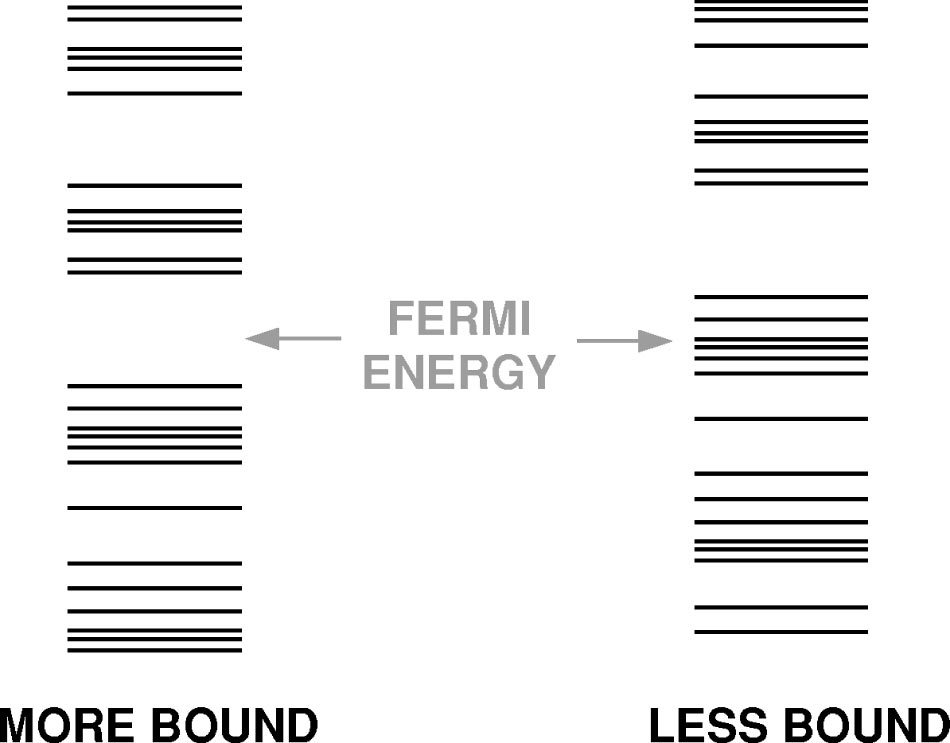
\includegraphics[width=0.5\textwidth]{Figure_1_Reimann}
    \caption{Bunching of the single-particles levels and level density at the Fermi level. From \cite{Brack1972}.}
	\label{fig:Figure_1_Reimann}
\end{figure}

It's very important to have a scheme of such energy levels, since it can immediately gives information about the stability of a system: if the level bunching at the Fermi surface has a minimum, then the system is more bound. In fact, this situation corresponds to particles occupying states with a lower energy (on average), thus minimizing the total energy. In terms of the shell-model, this means that all the shells below the Fermi level are filled (see Figure \ref{fig:Figure_1_Reimann}). A situation in which the level bunching doesn't have a minimum at the Fermi surface corresponds instead in a non-filled shell. In this case the system can rearrange itself in a non-symmetric shape, in order to reach a better stability.

This has been shown e.g. for atomic nuclei by means of nuclear spectroscopy. In that case, a measurement of the \emph{quadrupole moment} can exploit the possibly non symmetric structure. As a simple example, the quadruple moment $Q$ for a single proton is
\begin{equation}
	Q = e \int \psi^*(3z^2-r^2)\psi\,d\tau,
	\label{eq:quadrupole_single_proton}
\end{equation}
where $\tau$ indicates the volume. If $|\psi|^2$ is spherically symmetric, then -- on average -- $x^2=y^2=z^2=r^2/3$, and substituting $z^2=r^2/3$ into \eqref{eq:quadrupole_single_proton} gives zero \citep[see][]{Krane1988}. So, a non-zero quadrupole moment indicates a non-spherical shape; this shape can be determined by the analysis of the angular distribution of the radiation field.

But how can these deformations give a better stability to the system in the case of non-filled shells? The answer is simple: because they minimize the energy. To show this, we introduce the example of a two-dimensional anisotropic harmonic oscillator confinement of fermions \citep[as in][]{Reimann2002}, in which the effective potential is 
\begin{equation}
	V(x,y) = \frac{1}{2}m^*\omega^2\left(\delta x^2 + \frac{1}{\delta}y^2\right).
\end{equation}
Here $\omega$ is the oscillator frequency, $m^*$ is the effective mass of the fermions and the deformation parameter $\delta \doteqdot \omega_x/\omega_y$ is defined such that $\omega_x=\omega\sqrt{\delta}$ and $\omega_y=\omega/\sqrt{\delta}$. This condition guarantees that the area is conserved with the deformation. By analogy with the simple harmonic oscillator, which has energy levels $E_n = \hbar\omega(n+1/2)$, the energy levels of the 2D anisotropic case are just
\begin{equation}
	E_{n_x,n_y}(\delta) = \hbar\omega\left[\sqrt{\delta}\left(n_x+\frac{1}{2}\right) + \frac{1}{\sqrt{\delta}}\left(n_y+\frac{1}{2}\right)\right].
\end{equation}
These levels are plotted against the deformation in Figure \ref{fig:Figure_2_Reimann}. For $\delta=1$ (that is the isotropic case) you see that there is a $(n+1)$-fold degeneracy, where $n=n_x+n_y=0,1,2,\ldots$ is the principal quantum number. Taking into account the spin degeneracy (that gives a factor 2), we obtain closed shells for $N=2,6,12,20,\ldots$ electrons. These numbers are called the \emph{magic numbers}. As we increase the deformation parameter, the degenerate levels split. It is useful, in this case, to look at the total energies (on the right in Figure \ref{fig:Figure_2_Reimann}); you see that now the energy levels have cups and minima that significantly change the behavior of the system for non-closed shells. In fact the energies have minima at $\delta=1$ for the closed-shell cases ($N=2,6,12$), whereas their minima are shifted to different values of $\delta$ in the open-shell cases ($N=4,8,10$). As a rough graphical estimate, for $N=4$ the minimum energy (i.e., the stablest configuration) is reached about a deformation value $\delta=2$ and for $N=10$ about $\delta=1.5$.

\begin{figure}[H]
	\centering
    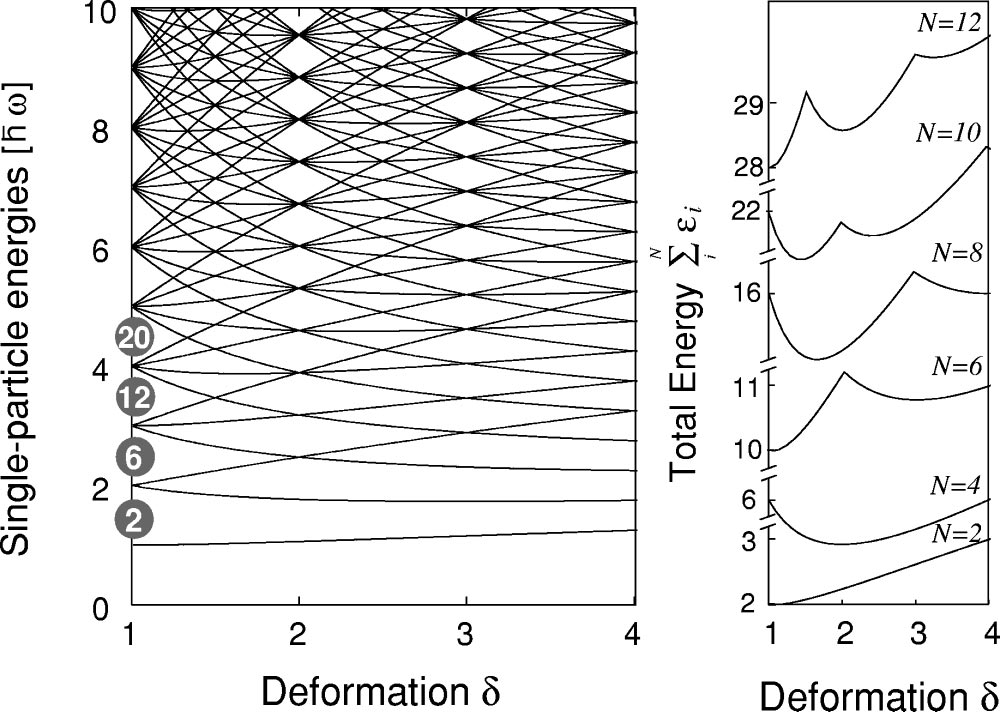
\includegraphics[width=0.65\textwidth]{Figure_2_Reimann}
    \caption{Single particle energy levels (left) and total energies (right) as a function of the deformation in a two-dimensional harmonic oscillator. From \cite{Reimann2002}.}
	\label{fig:Figure_2_Reimann}
\end{figure}

Even this simple example shows in an effective way how a deformation can guarantee a stabler configuration for non-closed shells. Further in our simulations, we will restrict only to closed-shell systems.

\section{Evidences of the shell-model}
\label{sec:shell_model_evidences}
We said before that the shell-structure seems to be a common property of finite fermion systems. Indeed, clear evidences of it had been shown for \emph{atoms}, \emph{atomic nuclei}, \emph{clusters of atoms} and \emph{quantum dots}. Let's briefly see which kind of measurements led to this results.

\begin{figure}[h]%[H]
	\centering
    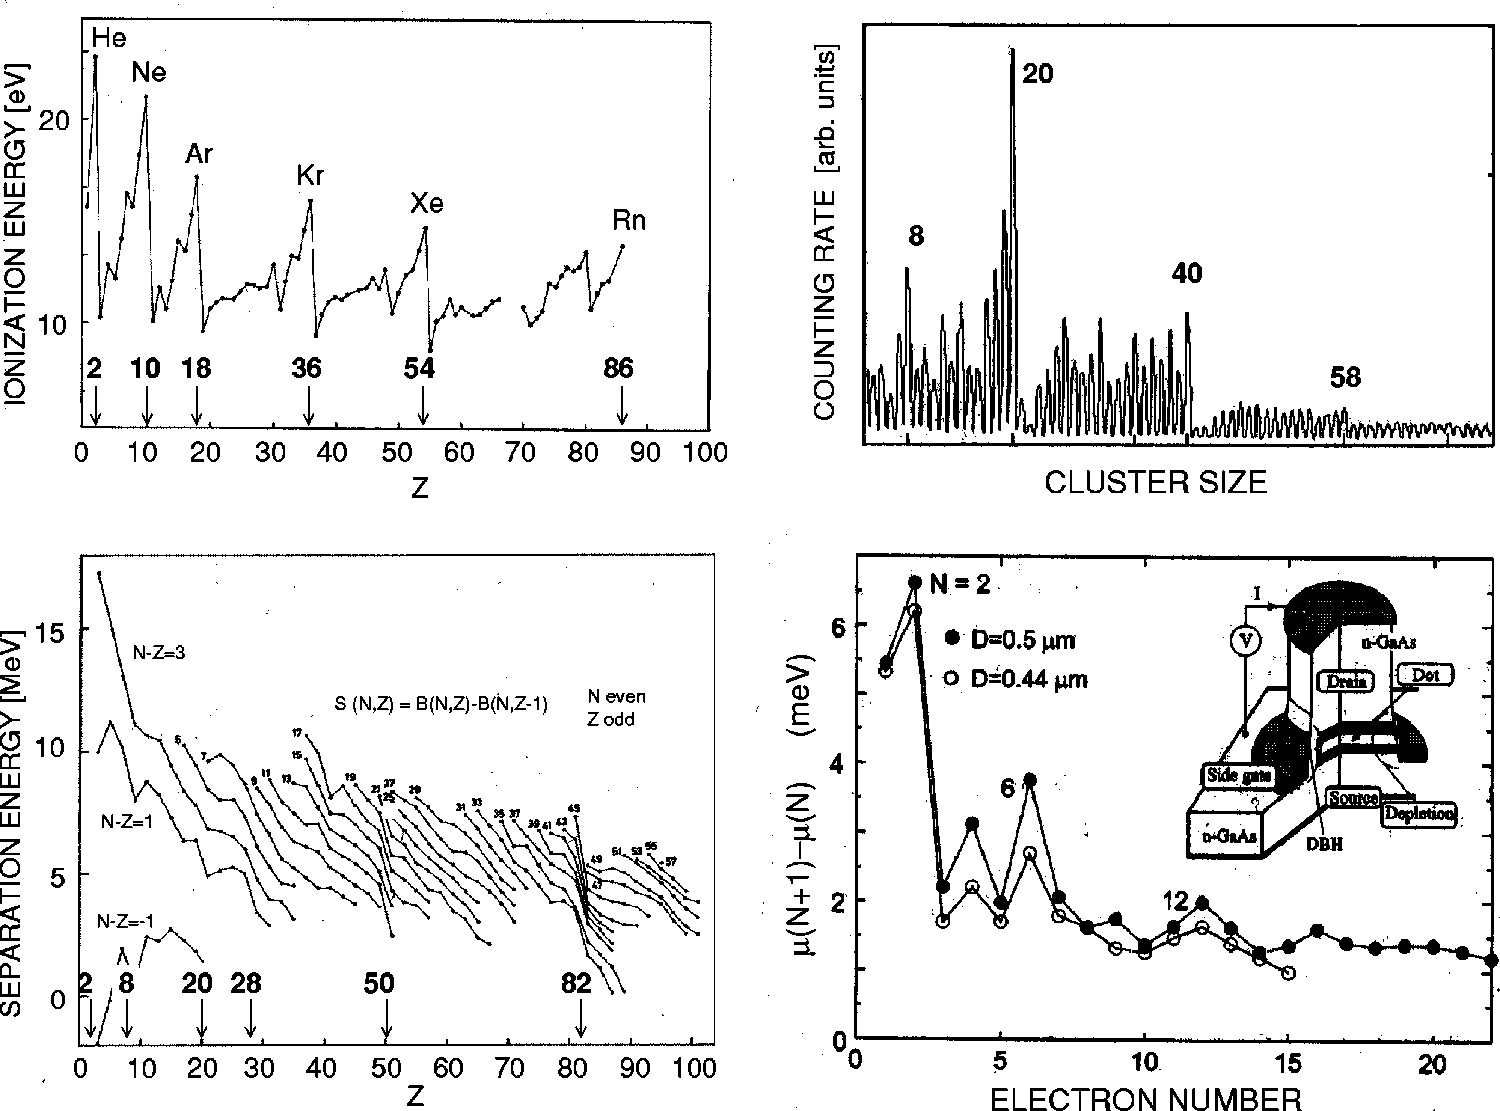
\includegraphics[width=\textwidth]{Figure_3_Reimann}
    \caption{Upper left, atomic ionization energies; lower left, separation energies of atomic nuclei; upper right, abundance spectra of metallic clusters; lower right, addition energies in a
disk-shaped quantum dot (schematized in the inset). From \cite{Reimann2002}.}
	\label{fig:Figure_3_Reimann}
\end{figure}

In the case of atoms, the shell-model is applied to the electrons ``orbiting'' around the nucleus, which is considered as an effective attractive Coulomb potential. A very natural quantity that one may think to measure in order to exploit the shell structure is the \emph{ionization energy}, that is the energy required to remove an electron from a neutral atom. In fact we have shown that electrons in a closed-shell system are more bound, which means that we expect to need more energy to remove one of it (i.e., we expect to see a higher ionization energy). Indeed this happens pretty clearly, as you see in Figure \ref{fig:Figure_3_Reimann}, upper left, showing the sequence of magic numbers $N=2,10,18,36,54,86,\ldots$.

For atomic nuclei the idea is quite the same, with the only difference that now we have to measure the energy required to remove a nucleon from the nucleus (which is called the \emph{separation energy}). The step-like behavior is also present in this case, giving the sequence of magic numbers $N=2,8,20,28,50,82,\ldots$ (Figure \ref{fig:Figure_3_Reimann}, lower left).

Atomic clusters are also an interesting case, since they show anomalies in the mass abundance spectra: for certain cluster sizes, the clusters are more stable. This behavior has been explained with the ``jellium'' theory for metallic clusters; the valence electrons are treated as trapped in a homogeneous positive-charged background (the jellium), that stems from the atomic ions. Density functional calculations showed the magic number sequence $N=2,8,20,40,58$ (see Figure \ref{fig:Figure_3_Reimann}, upper right) some years before it was discovered with experiments in the beginning of the 80's \citep[see][]{Reimann2002}.

The sequence of magic numbers for quantum dots was discovered in 1996 by using an etched pillar of semiconducting material as shown in Figure \ref{fig:Figure_3_Reimann}, lower right \citep[see also][]{Tarucha1996}. As we will see later, a quantum dot can be schematized as a one-electron transistor; measurements of the energy needed to add a single electron to a $N$-electrons quantum dot show large peaks for $N=2,6,12$ (Figure \ref{fig:Figure_3_Reimann}). Noticeably, these numbers are the same quantum numbers obtained for a two-dimensional harmonic oscillator.

\section{The Coulomb blockade model}
% Refer to it as model or effect? Found both of them.

\begin{figure}[h]%[H]
	\centering
    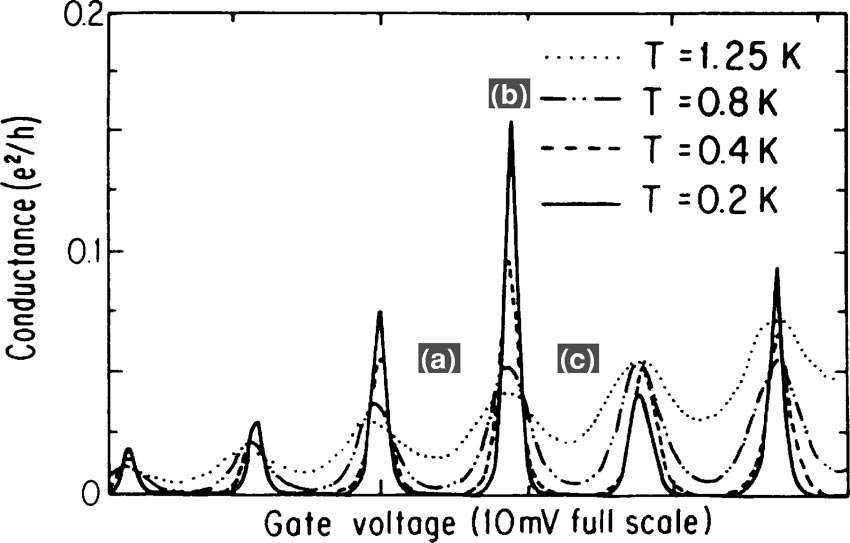
\includegraphics[width=0.60\textwidth]{Figure_6_Reimann}
    \caption{Coulomb oscillations in a lateral quantum dot. The regions (a) and (c) have a fixed number of electrons since there is a Coulomb blockade; (b) is the conductance region, where the number of electrons oscillates. Plot based on the work of \cite{Meirav1990}, by \cite{Meir1991}.}
	\label{fig:Figure_6_Reimann}
\end{figure}

The behavior of a quantum dot can be analyzed by studying its electron transport mechanism. In order to do that, the dot is connected to a circuit that provides a certain gate voltage, and its conductance is measured. A plot like the one in Figure \ref{fig:Figure_6_Reimann} is obtained; you see that there are conductance peaks at specific gate voltages, all of them evenly spaced. This behavior can be explained by the \emph{Coulomb blockade model}.

% Usage: 
\newcommand{\trcomponent}[2]
{
	\draw (#1) node[align=center] {\textnormal #2};
}

% Usage: \circlecomp{position}{text}
\newcommand{\circlecomp}[2]
{
	\draw[thick] (#1) node[draw,shape=circle,scale=0.85,align=center] {#2};
}

\newcommand{\vertcomp}[2]
{
\draw[thick] (#1) node[draw,shape=rectangle,scale=1,align=center] {\textnormal #2};
}

\begin{figure}[h]%[H]
	\centering
	\begin{circuitikz}[scale=1.1,transform shape]
		\draw (0,0) to (4,0) to (4,0.3) to[lamp,color=white,n=Vsd] ++(0,0.85);
		\draw (3.575,0.725) to (0.5,0.725) to (0.5,2.5)
			to[generic,bipoles/length=2cm,n=source] (2.5,2.5)
			to[C,l_=$C_1$,bipoles/length=1cm] (3,2.5)
			to[lamp,bipoles/length=2cm,color=white,n=dot] ++(2,0);
		\draw (4.425,0.725) to (7.5,0.725) to (7.5,2.5)
			to[generic,bipoles/length=2cm,n=drain] (5.5,2.5)
			to[C,l^=$C_2$,bipoles/length=1cm] (5,2.5);
		\draw (4,3.1) to[C,l=$C_3$,bipoles/length=1cm] (4,4.5)
			to[lamp,bipoles/length=0.9cm,color=white,n=gate] (4,5)
			to (4,5.3) to[lamp,bipoles/length=1.3cm,color=white,n=Vg] (0,5.3)
			to (0,0) node[ground] {};
		% Draw the components
		\circlecomp{Vsd}{$V_{\text{sd}}$}
		\trcomponent{source}{Source}
		\circlecomp{dot}{Dot\\$C_{\Sigma}$}
		\trcomponent{drain}{Drain}
		\vertcomp{gate}{Gate}
		\circlecomp{Vg}{$V_{\text{g}}$}
		% Draw the intrinstic indicators
		\draw[dashed] (0.4,1.5) rectangle (3.2,3.1);
		\draw[dashed] (7.6,1.5) rectangle (4.8,3.1);
		\draw[dashed] (3,3.5) rectangle (5,5.4);
	\end{circuitikz}
	\caption{Scheme of a single electron transistor. The island has index 0, the source has index 1, the drain index 2 and the gate index 3. The capacitances are meant to be intrinsic capacitances of the respective electrode (source, drain or gate). Adapted from \cite{Fasth2007}.}
	\label{fig:SET_scheme}
\end{figure}

Let's consider a \emph{single-electron transistor} device, like the one in Figure \ref{fig:SET_scheme}. This name is due to the fact that the charge on the electron island is a multiple of the elementary charge. The electron island is weakly coupled with the source and drain contacts thanks to tunnel barriers, which are thick enough to guarantee that quantum resonances dominates the electron transport mechanism.; in other words, the conductance of the tunnel must be smaller than the quantum conductance $e^2/h$ \citep[see][]{Reimann2002}. By analogy with a capacitor, in which the energy stored is $U=Q^2/2C$, one can make a first estimate of the energy stored in a dot containing $N$ particles as
\begin{equation}
	U(N) \simeq \frac{N(N-1)}{2C_{\Sigma}}.
\end{equation}
Here, the factor $(N-1)$ takes into account that each electron interacts with $N-1$ neighbors. Using this rough estimate, one can say that the energy required to add a single electron to a system already confining $N$ electrons, called the \emph{addition energy}, is
\begin{equation}
	\Delta U (N) = U(N+1)-U(N) = \frac{N(N+1)e^2}{2C_{\Sigma}} - \frac{N(N-1)e^2}{2C_{\Sigma}} = \frac{Ne^2}{C_{\Sigma}}.
\end{equation}
You see that, for successive $N$'s, the energy values are separated by the so-called \emph{charging energy}, $e^2/C_{\Sigma}$, which is constant. At low enough temperatures and bias voltages, the charging energy might be larger than the thermal energy ($e^2/C_{\Sigma} \gg k_BT$), thus preventing the electrons from tunneling the barriers. In this case transport is blocked, and this effect is called the \emph{Coulomb blockade}.

Let's now analyze the same situation in a more precise way \citep[adapted from][]{Fasth2007}. If we label the dot with the index $i=0$, the source with 1, the drain with 2 and the gate with 3, the induced charge $\tilde{Q}_i$ on each of the electrodes can be written as
\begin{equation}
	\tilde{Q}_i = \sum_{j=0}^{n}C_{ij}V_j,
\end{equation}
where $C_{ij}$ is the capacitance matrix, $V_j$ is the potential on the $j$'th element, and $n$ will be in general larger than 3 because of additional gate electrodes. If we refer to the dot ($i=0$), we can then write
\begin{equation}
	\tilde{Q}_0 = \sum_{j=0}^{n}C_{0j}V_j = C_{00}V_0 + \sum_{j=1}^{n}C_{0j}V_j,
\end{equation}
from which
\begin{equation}
	V_0 = \frac{1}{C_{00}}\left(\tilde{Q}_0 - \sum_{j=1}^{n}C_{0j}V_j\right).
	\label{eq:V0_vs_Q0tilde}
\end{equation}
In general, the induced charge $\tilde{Q}_0$ will be not equal to the measured one, $Q_0$, because of the presence of a background charge $Q_{\text{bg}}$ (that can be measured if all the potentials are set to zero). This means that $\tilde{Q}_0 = Q_0 - Q_{\text{bg}}$. Moreover, $C_{\Sigma} \equiv C_{00}$ by definition, and we can find an expression for it using the charge neutrality condition $\sum_{j=0}^{n}C_{0j}=0$, which implies $C_{\Sigma} \equiv C_{00} = -\sum_{j=1}^{n}C_{0j}$. Using these two facts, we can rewrite equation \eqref{eq:V0_vs_Q0tilde} as
\begin{equation}
	V_0(Q_0) = \frac{1}{C_{\Sigma}}\left(Q_0 - Q_{\text{bg}} - \sum_{j=1}^{n}C_{0j}V_j\right).
	\label{eq:V0_vs_Q0}
\end{equation}

At this point, we can calculate the energy $U(N)$ stored in a dot with $N$ electrons by performing an integration:
\begin{equation}
	U(N) = \int_{0}^{-eN}V_0(Q_0)\,dQ_0 = \frac{e^2N^2}{2C_{\Sigma}} + eN\left( \frac{Q_{\text{bg}}}{C_{\Sigma}} + \sum_{j=1}^{n}\frac{C_{0j}}{C_{\Sigma}}V_j \right).
\end{equation}

Using this expression, we can finally calculate the addition energy as
\begin{equation}
	\Delta U (N) = U(N+1)-U(N) = \frac{e^2}{C_{\Sigma}}\left(N+\frac{1}{2}\right) + e\left( \frac{Q_{\text{bg}}}{C_{\Sigma}} + \sum_{j=1}^{n}\frac{C_{0j}}{C_{\Sigma}}V_j \right).
\end{equation}
You see that, for small temperatures and bias voltages, we can approximate $\Delta U (N) \simeq e^2N/C$ as we found previously by a rough estimate.

This calculation still lacks the fact that, in such a small device, quantization effects are also important and should be considered. A simple model that combines the Coulomb blockade effect and the quantum effects is the \emph{constant interaction model}.

\section{The constant interaction model}
The basis assumption of the constant interaction model is that the total energy $E(N)$ of the electron island is the sum of the single-particle energies and the electrostatic energy $U(N)$:
\begin{equation}
	E(N) = \sum_{i=1}^{N}\epsilon_i + U(N) = \sum_{i=1}^{N}\epsilon_i + \frac{e^2N^2}{2C_{\Sigma}} + eN\left( \frac{Q_{\text{bg}}}{C_{\Sigma}} + \sum_{j=1}^{n}\frac{C_{0j}}{C_{\Sigma}}V_j \right).
\end{equation}
From this expression we can calculate the \emph{electrochemical potential} $\mu_N$, that is defined as the necessary energy to add the $N$-th electron to a conductor, as
\begin{equation}
	\mu_N 
	= E(N) - E(N-1) 
	=  \epsilon_N + \frac{e^2}{C_{\Sigma}}\left(N-\frac{1}{2}\right) + e\left( \frac{Q_{\text{bg}}}{C_{\Sigma}} - \sum_{j=1}^{n}\alpha_jV_j \right),
	\label{eq:electrochemical_potential}
\end{equation}
where $\alpha_j$, defined as
\begin{equation}
	\alpha_j \doteqdot - \frac{C_{0j}}{C_{\Sigma}},
\end{equation}
is called the \emph{lever arm} of the gate $j$ and is always positive. Experiments show that the lever arm changes in a significant way only for very large gate voltage variations; so, in most cases the lever arm can be considered constant \citep{Fasth2007}. This implies that the relation between the electrochemical potential and the gate voltage in equation \eqref{eq:electrochemical_potential} is linear; an increase in the gate voltage reflects in a decrease of the electrochemical potential, and vice-versa.

One can also calculate the spacing between different $\mu_N$'s, that is
\begin{equation}
	\mu_{N+1}-\mu_N 
	= \epsilon_{N+1} - \epsilon_{N} + \frac{e^2}{C_{\Sigma}}
	= \Delta_{N+1} + \frac{e^2}{C_{\Sigma}},
\end{equation}
where $\Delta_{N+1}\doteqdot \epsilon_{N+1} - \epsilon_{N}$ is the spacing between two successive single-particles energy levels. You immediately note that, when $\Delta_{N+1} \ll k_BT \ll e^2/C_{\Sigma}$, the quantum effects can be neglected and the Coulomb blockade oscillations are periodic in $e^2/C_{\Sigma}$ \citep{Reimann2002}.

\begin{figure}
	\centering
	\begin{subfigure}[t]{0.45\textwidth}
		\newcommand{\ThickBorder}{(0,3) -- (2.8,3) -- (2.8,9) -- (3.2,9) -- (3.2,1) -- (5.8,1) -- (5.8,8.6) -- (6.2,8.6) -- (6.2,2.5) -- (9,2.5)}
		\begin{tikzpicture}[scale=0.8]%every node/.style={transform shape}
			\tikzset{>=latex}
			
			% Fill dark region
			\fill[draw=none,fill=black!40!white]
				(0,0) -- \ThickBorder -- (9,0) -- cycle;
				
			%Fill light regions
			\fill[draw=none,fill=black!10!white]
				(0,3) -- (2.8,3) -- (2.8,6) -- (0,6) -- cycle;
			\fill[draw=none,fill=black!10!white]
				(3.2,1) -- (5.8,1) -- (5.8,5) -- (3.2,5) -- cycle;
			\fill[draw=none,fill=black!10!white]
				(6.2,2.5) -- (9,2.5) -- (9,5.6) -- (6.2,5.6) -- cycle;
				
			% Draw thick border
			\draw[thick] \ThickBorder;
			
			% Draw source potential
			\draw[very thick] (0,6) -- (2.8,6) node[midway,above] {$\mu_S$};
			
			% Draw dot potential
			\draw[very thick] (3.2,5) -- (5.8,5) node[midway,above] {$\mu_N$};
			\draw[very thick, dashed] (3.2,7.2) -- (5.8,7.2) node[midway,above] {$\mu_{N+1}$};
			 
			% Draw drain potential
			\draw[very thick] (6.2,5.6) -- (9,5.6) node[midway,above] {$\mu_D$};
			
			% Draw units
			\draw[<->, thick] (5,5) -- (5,7.2)
				node[midway,fill=white,text=black,xshift=-0.4cm,yshift=0.05cm]
				{\scriptsize $\dfrac{e^2}{C_{\Sigma}} + \Delta_{N+1}$};
			\draw[<->, thick] (6.4,1) -- (6.4,2.5)
				node[midway,fill=black!40!white,text=black,xshift=+0.45cm]
				{\scriptsize $U_{N+1}(V_G)$};
			 
		\end{tikzpicture}	
		\caption{$\mu_N<\mu_D$: the transport is blocked due to the Coulomb blockade. The number of electrons inside the dot is $N$.}
		\label{fig:SET_mu_potential_stage1}
	\end{subfigure}
	$\qquad$
	\begin{subfigure}[t]{0.45\textwidth}
		\newcommand{\ThickBorderUp}{(0,3) -- (2.8,3) -- (2.8,9) -- (3.2,9) -- (3.2,1.8) -- (5.8,1.8) -- (5.8,8.5) -- (6.2,8.5) -- (6.2,2.5) -- (9,2.5)}
		\begin{tikzpicture}[scale=0.8]%every node/.style={transform shape}
			\tikzset{>=latex}
			
			% Fill dark region
			\fill[draw=none,fill=black!40!white]
				(0,0) -- \ThickBorderUp -- (9,0) -- cycle;
				
			%Fill light regions
			\fill[draw=none,fill=black!10!white]
				(0,3) -- (2.8,3) -- (2.8,6) -- (0,6) -- cycle;
			\fill[draw=none,fill=black!10!white]
				(3.2,1.8) -- (5.8,1.8) -- (5.8,3.6) -- (3.2,3.6) -- cycle;
			\fill[draw=none,pattern=north east lines,pattern color=black!10!white]
				(3.2,3.6) -- (5.8,3.6) -- (5.8,5.8) -- (3.2,5.8) -- cycle;
			\fill[draw=none,fill=black!10!white]
				(6.2,2.5) -- (9,2.5) -- (9,5.6) -- (6.2,5.6) -- cycle;
				
			% Draw thick border
			\draw[thick] \ThickBorderUp;
			
			% Draw source potential
			\draw[very thick] (0,6) -- (2.8,6) node[midway,above] {$\mu_S$};
			
			% Draw dot potential
			\draw[very thick] (3.2,5.8) -- (5.8,5.8) node[midway,above] {$\mu_N$};
			\draw[very thick] (3.2,3.6) -- (5.8,3.6) node[midway,above] {$\mu_{N-1}$};
			 
			% Draw drain potential
			\draw[very thick] (6.2,5.6) -- (9,5.6) node[midway,above] {$\mu_D$};
			
			% Draw units
			\draw[<->, thick] (6.4,1.8) -- (6.4,2.5)
				node[midway,fill=black!40!white,text=black,xshift=+0.80cm,yshift=-0.02cm]
				{\scriptsize $U_{N}(V_G)$};
			 
		\end{tikzpicture}	
		\caption{$\mu_S \gtrsim \mu_N \gtrsim \mu_D$: one electron can tunnel the barrier. The number of electrons inside the dot varies from $N-1$ to $N$. This configuration is obtain by lowering $V_G$, in order to increase $\mu_N$.}
		\label{fig:SET_mu_potential_stage2}	
	\end{subfigure}
	\begin{subfigure}[t]{0.45\textwidth}
		\newcommand{\ThickBorderUp}{(0,3) -- (2.8,3) -- (2.8,9) -- (3.2,9) -- (3.2,2.4) -- (5.8,2.4) -- (5.8,8.5) -- (6.2,8.5) -- (6.2,2.5) -- (9,2.5)}
		\begin{tikzpicture}[scale=0.8]%every node/.style={transform shape}
			\tikzset{>=latex}
			
			% Fill dark region
			\fill[draw=none,fill=black!40!white]
				(0,0) -- \ThickBorderUp -- (9,0) -- cycle;
				
			%Fill light regions
			\fill[draw=none,fill=black!10!white]
				(0,3) -- (2.8,3) -- (2.8,6) -- (0,6) -- cycle;
			\fill[draw=none,fill=black!10!white]
				(3.2,2.4) -- (5.8,2.4) -- (5.8,4.2) -- (3.2,4.2) -- cycle;
			\fill[draw=none,fill=black!10!white]
				(6.2,2.5) -- (9,2.5) -- (9,5.6) -- (6.2,5.6) -- cycle;
				
			% Draw thick border
			\draw[thick] \ThickBorderUp;
			
			% Draw source potential
			\draw[very thick] (0,6) -- (2.8,6) node[midway,above] {$\mu_S$};
			
			% Draw dot potential
			\draw[very thick, dashed] (3.2,6.4) -- (5.8,6.4) node[midway,above] {$\mu_N$};
			\draw[very thick] (3.2,4.2) -- (5.8,4.2) node[midway,above] {$\mu_{N-1}$};
			 
			% Draw drain potential
			\draw[very thick] (6.2,5.6) -- (9,5.6) node[midway,above] {$\mu_D$};
			 
		\end{tikzpicture}	
		\caption{$\mu_N>\mu_S$: the transport is blocked again due to the Coulomb blockade. The number of electrons inside the dot is $N-1$. This situation is obtained by further lowering $V_G$.}
		\label{fig:SET_mu_potential_stage3}
		\end{subfigure}
	\caption{Energy diagram of a quantum dot. The sequence of images illustrates the transport process of the electrons \citep[adapted from][]{Fasth2007}.}
	\label{fig:SET_mu_potential}
\end{figure}

Using this information, we can now analyze the transport mechanism in a quantum dot. Let's consider -- as explained before -- the low-temperature, low-bias voltage case ($eV_{\text{bias}},k_BT \ll e^2/C_{\Sigma}$). Let's also suppose that, initially, the electrochemical potential inside the dot -- $\mu_N$ -- is lower than the electrochemical potential of the drain -- $\mu_D$: the transport is blocked due to the Coulomb blockade effect (Figure \ref{fig:SET_mu_potential_stage1}). Now, we can decrease the gate voltage: the overall effect, as you can see from equation \eqref{eq:electrochemical_potential} and from our previous considerations, is that we have a linear increase in $\mu_N$ wrt the gate voltage. Eventually, $\mu_N$ will align to $\mu_D$ ($\mu_N = \mu_D$), which means that an electron can leave the dot. At the same time, if $\mu_S \gtrsim \mu_D$, an electron from $\mu_S$ can enter the dot; the overall effect is that the number of the electrons inside the dot oscillates between $N$ and $N-1$, and an electric current flows though the dot from the drain to the source (Figure \ref{fig:SET_mu_potential_stage2}). In terms of the conductance, this corresponds in a peak. If we keep lowering the gate voltage -- i.e., increasing $\mu_N$ -- until $\mu_N > \mu_S$, then the dot is left with only $N-1$ electrons. Now, the level to consider is $\mu_{N-1}$: you see that it's far below $\mu_D$, so the current is blocked again (see Figure \ref{fig:SET_mu_potential_stage3}).

This qualitative analysis also permits to find the gate voltage values for which we have peaks in the conductance. The peak condition, in fact, is $\mu_S\approx\mu_N\approx\mu_D$; inserting this condition in \eqref{eq:electrochemical_potential} and solving for $V_3$ (the index 3 indicates the gate, so we will replace the subscript with ``G'' for simplicity) gives
\begin{align}
	V_G^{(N)}
	&\approx \frac{1}{e\alpha_G}\left[ \epsilon_N + \frac{e^2}{C_{\Sigma}}\left(N-\frac{1}{2}\right) + \frac{eQ_{\text{bg}}}{C_{\Sigma}} - \mu_S - e\sum_{j=4}^{n}\alpha_jV_j - e\sum_{j=1}^{2}\alpha_jV_j \right] \\
	&\approx \frac{1}{e\alpha_G}\left[ \epsilon_N + \frac{e^2}{C_{\Sigma}}\left(N-\frac{1}{2}\right) + \frac{eQ_{\text{bg}}}{C_{\Sigma}} - \mu_S - e\sum_{j=4}^{n}\alpha_jV_j \right]
\end{align}
where the last term has been dropped because we are in the small-bias voltage case. The gate-voltage spacing between two peaks is finally found as (converted to energy)
\begin{align}
	e\Delta V_G(N) 
	&= e\Big[V_G^{(N)}-V_G^{(N-1)}\Big] \\
	&= \frac{1}{\alpha_G}\left( \epsilon_N - \epsilon_{N-1} + \frac{e^2}{C_{\Sigma}} \right) \\
	&= \frac{1}{\alpha_G}\left( \Delta_N + \frac{e^2}{C_{\Sigma}} \right).
	\label{eq:DeltaVG_N_Vb0}
\end{align}

As we already noticed before, for a lateral structure we can neglect the single-particle levels spacing (because the structure itself is quite large); this is not true for a vertical quantum dots structure, that has far smaller dimensions (as you can see in Figure \ref{fig:Figures_4-5_Reimann}). In that case the space quantization is evident and the conductance peaks are not evenly spaced, as you can see in Figure \ref{fig:Figure_10_Reimann}. It's also very nice that, by simply subtracting the quantity $1 / \alpha_G (e^2 / C_{\Sigma})$ from the spacing of two successive peaks, we can reconstruct the spectrum of the dot.

\begin{figure}[h]%[H]
	\centering
    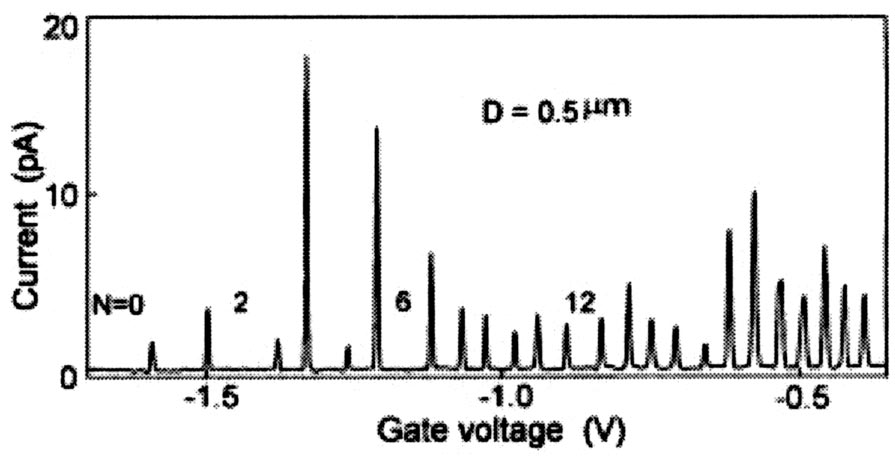
\includegraphics[width=0.55\textwidth]{Figure_10_Reimann}
    \caption{Coulomb oscillations in a vertical quantum dot. Here, $D$ is an estimate for the dot diameter. From \cite{Tarucha1996}.}
	\label{fig:Figure_10_Reimann}
\end{figure}

Finally, we briefly discuss the case in which the bias voltage cannot be neglected. Let's put us in the simple case of a symmetric bias voltage between the drain and the source, i.e.
\begin{equation}
	\begin{cases}
		V_S = V_{\text{bias}}/2 \\
		V_D = -V_{\text{bias}}/2
	\end{cases}
\end{equation}
which means that
\begin{equation}
	\begin{cases}
		\mu_S = \mu_0 + eV_{\text{bias}}/2 \\
		\mu_D = \mu_0 - eV_{\text{bias}}/2
	\end{cases}
\end{equation}
Here, $\mu_0$ is the electrochemical potential of both drain and source when the bias voltage is zero.

We showed before that the dot does not conduct for
\begin{equation}
	 \mu_N < \mu_D < \mu_S < \mu_{N+1}, \qquad V_{\text{bias}} > 0,
\end{equation}
and
\begin{equation}
	 \mu_N < \mu_S < \mu_D < \mu_{N+1}, \qquad V_{\text{bias}} < 0,
\end{equation}
so the borders of the Coulomb blockade region are defined by
\begin{equation}
	\mu_N = 
	\begin{cases}
		\mu_D = \mu_0 - eV_{\text{bias}}/2, & V_{\text{bias}} > 0 \\
		\mu_S = \mu_0 + eV_{\text{bias}}/2, & V_{\text{bias}} < 0
	\end{cases}
\end{equation}
and
\begin{equation}
	\mu_{N+1} = 
	\begin{cases}
		\mu_S = \mu_0 + eV_{\text{bias}}/2, & V_{\text{bias}} > 0 \\
		\mu_D = \mu_0 - eV_{\text{bias}}/2, & V_{\text{bias}} < 0
	\end{cases}
\end{equation}
Substituting these values for $\mu_N$, $V_S$ and $V_D$ in \eqref{eq:electrochemical_potential}, we finally find that the borders of the Coulomb blockade are the straight lines of equations
\begin{dmath}
	V_G^{(N)}(V_{\text{bias}})
	= \frac{1}{e\alpha_G}\left[ \epsilon_N + \frac{e^2}{C_{\Sigma}}\left(N-\frac{1}{2}\right) \\
	+ \frac{eQ_{\text{bg}}}{C_{\Sigma}} - \mu_0 - e(\alpha_S-\alpha_D-1)\frac{V_{\text{bias}}}{2} - e\sum_{j=4}^{n}\alpha_jV_j \right]
	\label{eq:VG_N}
\end{dmath}
and
\begin{dmath}
	V_G^{(N+1)}(V_{\text{bias}})
	= \frac{1}{e\alpha_G}\left[ \epsilon_{N+1} + \frac{e^2}{C_{\Sigma}}\left(N+\frac{1}{2}\right) \\
	+ \frac{eQ_{\text{bg}}}{C_{\Sigma}} - \mu_0 - e(\alpha_S-\alpha_D+1)\frac{V_{\text{bias}}}{2} - e\sum_{j=4}^{n}\alpha_jV_j \right]
	\label{eq:VG_N+1}
\end{dmath}
for $V_{\text{bias}}>0$. The case $V_{\text{bias}}<0$ is handled similarly.

By equating \eqref{eq:VG_N} and \eqref{eq:VG_N+1} we find that these two lines cross at $eV_{\text{bias}} = \Delta_{N+1} + e^2/C_{\Sigma}$, where $\Delta_{N+1}=\varepsilon_{N+1}-\varepsilon_{N}$ as usual. For $V_{\text{bias}}=0$, instead, we find that the spacing between $V_G^{(N)}$ and $V_G^{(N+1)}$ is $(\Delta_{N+1} + e^2/C_{\Sigma})/\alpha_G$ as we found previously for a negligible $V_{\text{bias}}$, equation \eqref{eq:DeltaVG_N_Vb0}. The situation is schematically pictured in Figure \ref{fig:diamond_regions}.

\begin{figure}[h]%[H]
	\centering
	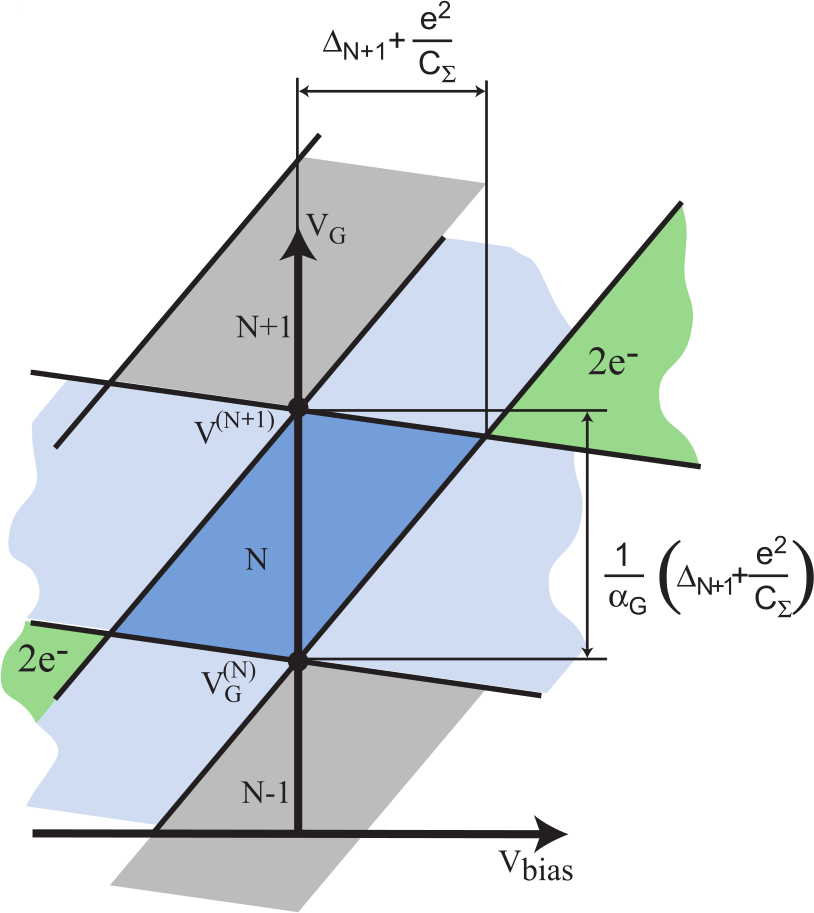
\includegraphics[width=0.5\textwidth]{diamond_regions}
	\caption{Coulomb blockade diamonds (gray and dark blue regions). In the dark blue region, the probability of finding $N$ electrons in the dot is $1$ (stable configuration); in the light blue regions, the probability varies from 0 to 1 and the electron number can change by one. In the green region, the bias voltage is so high that eventually $eV_{\text{bias}} > e^2/C_{\Sigma}$; due to this fact, two electrons can tunnel at the same time. From \cite{Fasth2007}.}
	\label{fig:diamond_regions}
\end{figure}

The diamond-shaped structure shown in Figure \ref{fig:diamond_regions} have been shown in differential conductance measurements like the one shown in Figure \ref{fig:Figure_8_Reimann}. A 3D elaboration of the data obtained from this kind of experiment -- that clarifies the ideas a little bit -- is shown in Figure \ref{fig:diff_conductance_3D}.

\begin{figure}[H]
	\centering
	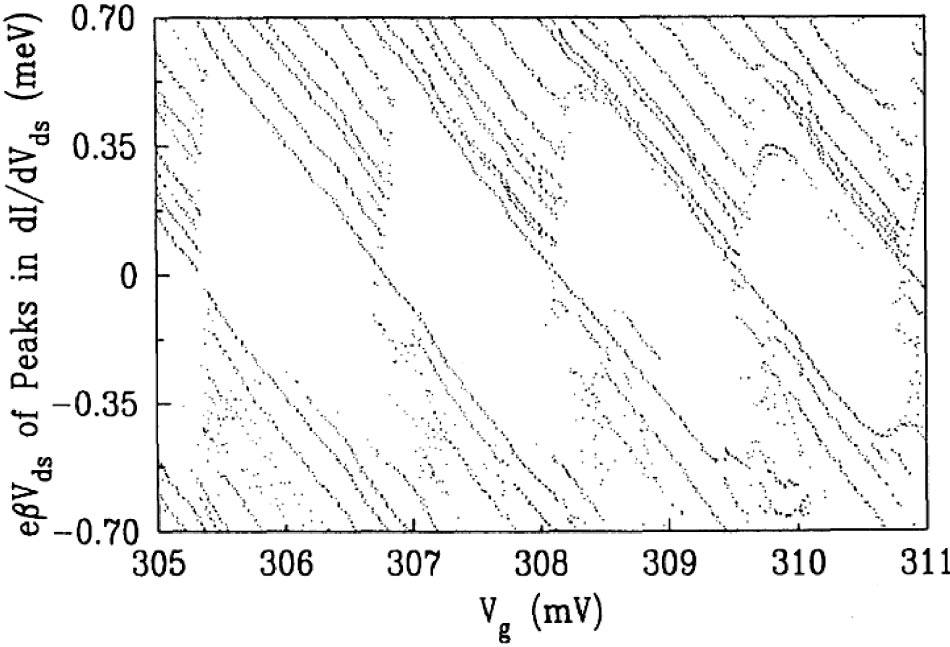
\includegraphics[width=0.6\textwidth]{Figure_8_Reimann}
	\caption{Peaks in the differential conductance $\partial I/\partial V_{\text{sd}}$ (showed as solid lines) of a lateral quantum dot, as a function of $V_{\text{sd}}$ and $V_{\text{g}}$. The white regions are the Coulomb blockade regions; between successive regions, the number of electrons in the dot is increased by one. From \cite{Reimann2002}.}
	\label{fig:Figure_8_Reimann}
\end{figure}

\begin{figure}[H]
	\centering
	\def\svgwidth{0.8\textwidth}
	\input{Mainmatter/figures/diff_conductance_3D.pdf_tex}
	\caption{Differential conductance $\partial I/\partial V_{\text{sd}}$ in a nanowire, plotted against $V_{\text{sd}}$ and $V_{\text{g}}$. Green and red indicate positive values; blue means close to zero, whereas pink stands for negative. From \cite{Weinmann1994}.}
	\label{fig:diff_conductance_3D}
\end{figure}

\section{The parabolic confinement}
In our simulation, we will model the confining (single-particle) potential as a \emph{two-dimensional harmonic trap}. This form for the confining potential is widely accepted as a standard for both exact and effective-field calculations, and is the result of experimental observations and numerical calculations.

The basis for this assumption can be found in the work of \cite{Kumar1990}. They performed numerical calculations on the Poisson and Schr\"{o}dinger equations to obtain the electron states in a GaAs/AlGaAs quantum dot -- like the one sketched in Figure \ref{fig:Figure_5_Reimann}. The calculations were done in the Hartree approximation. The results were quite interesting, as you can see in Figure \ref{fig:Figure_2_Kumar}; despite the square shape of the GaAs cap, the contours of the effective confinement potential were circular.

\begin{figure}[h]%[H]
	\centering
	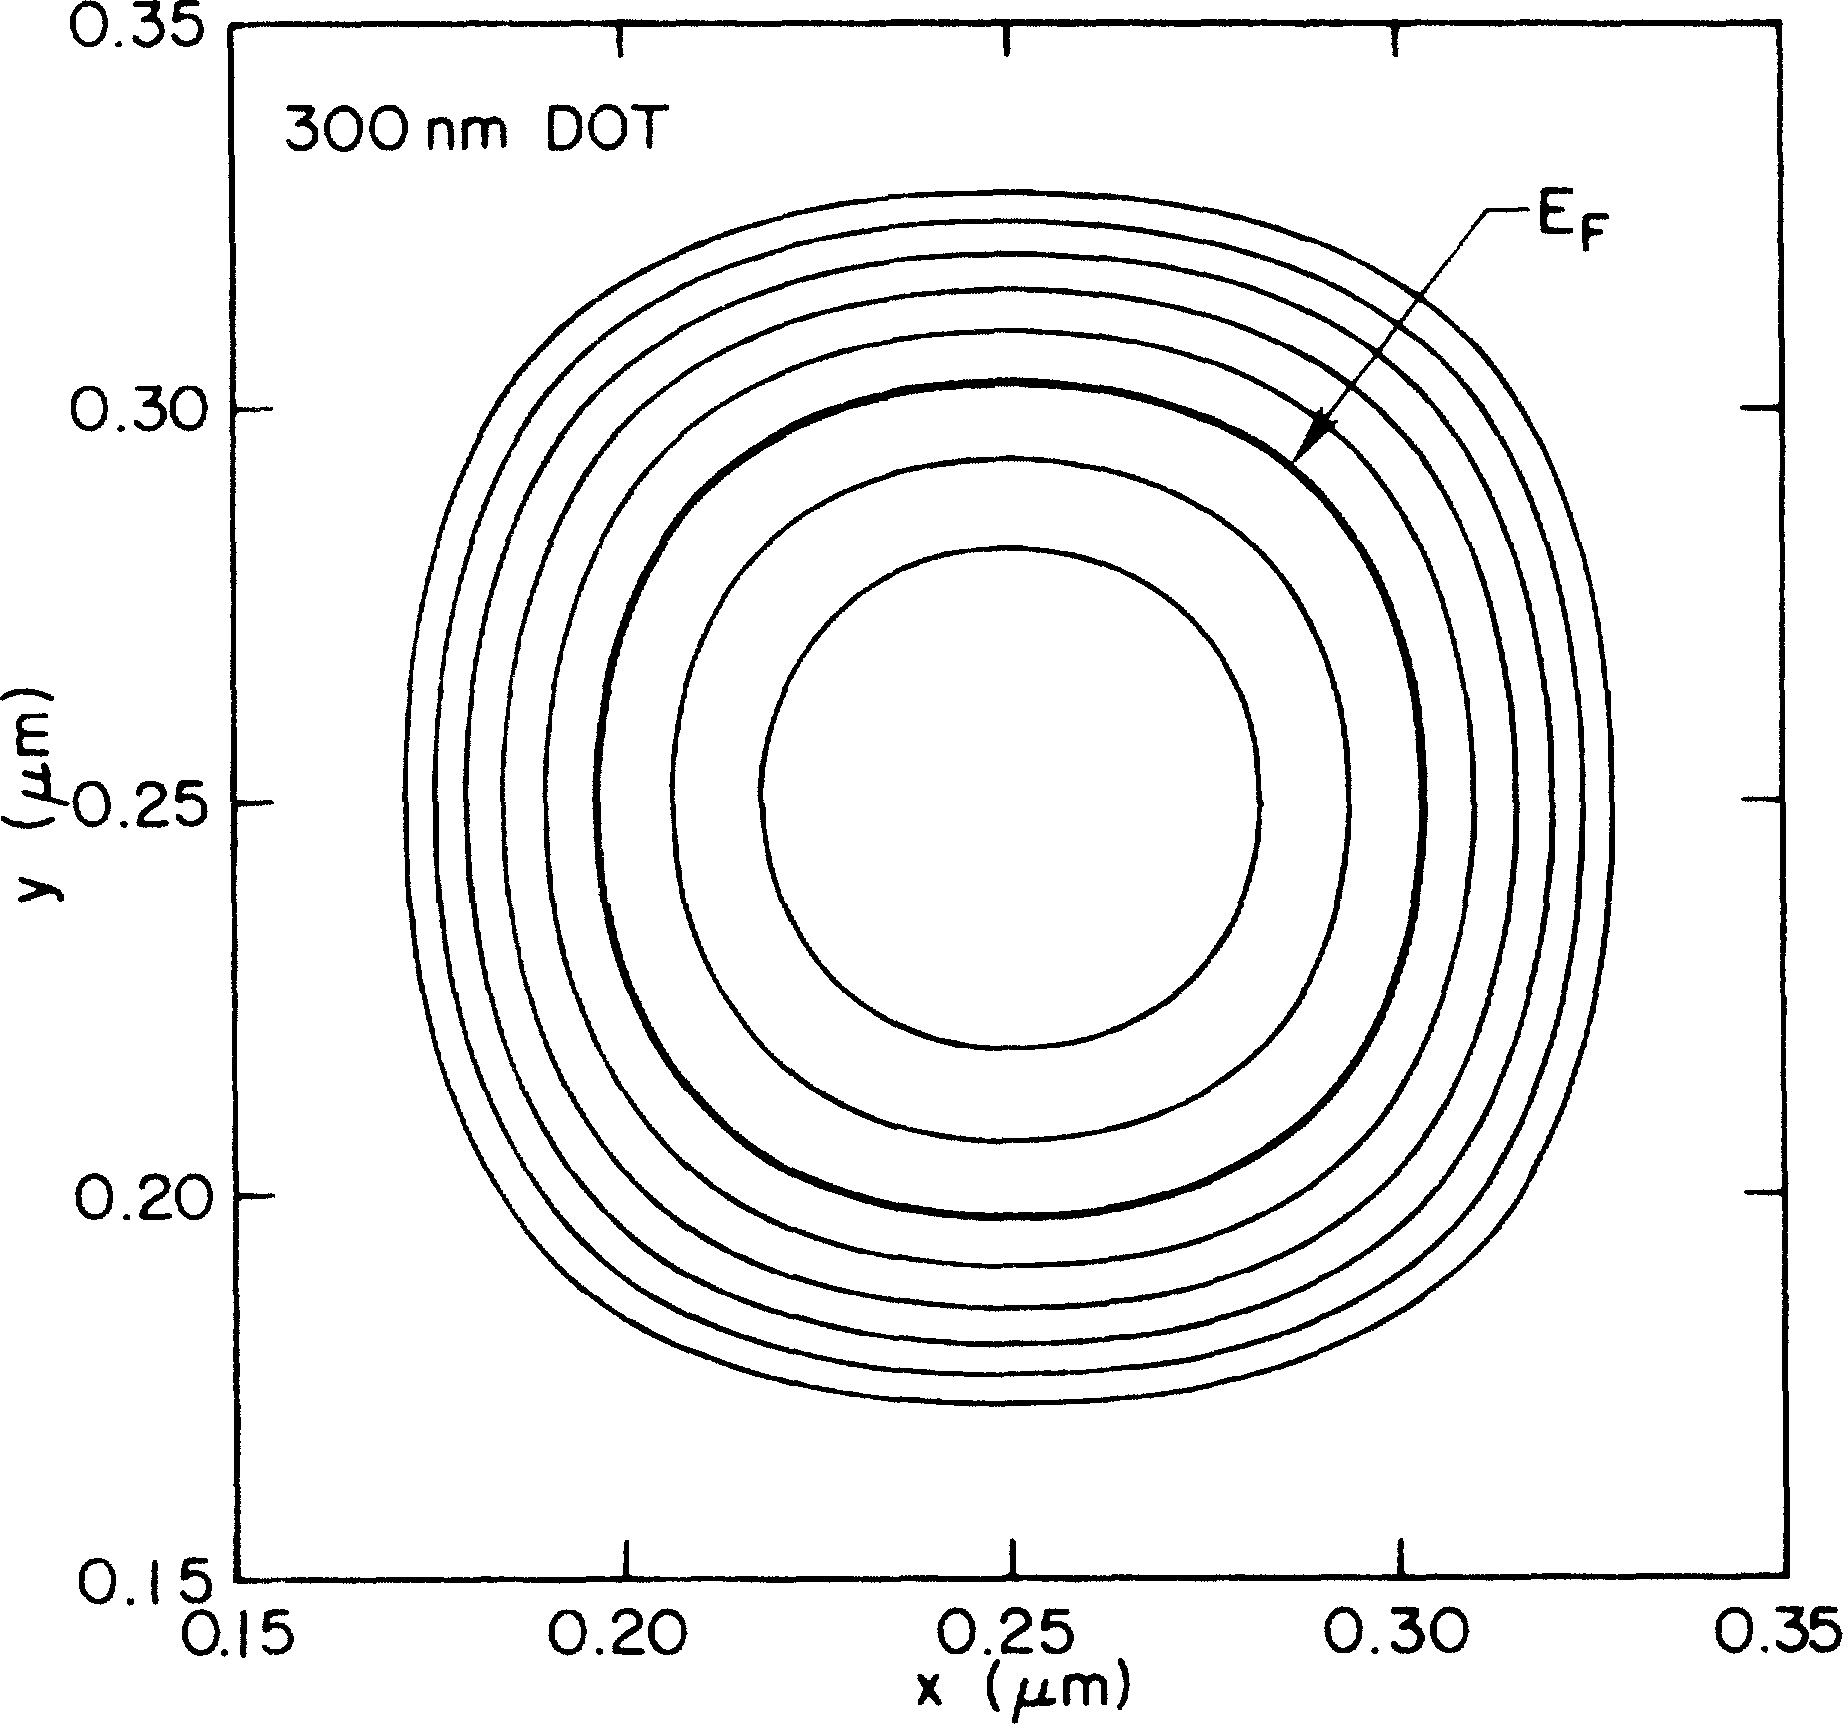
\includegraphics[width=0.55\textwidth]{Figure_2_Kumar}
	\caption{Contours of the lateral potential in a GaAs/AlGaAs quantum dot. The measurements were taken $\SI{8}{\milli\meter}$ below the contact surface of the two materials, and the contours are evenly separated by $\SI{10}{\milli e\volt}$ intervals. The Fermi level (thick line) is indicated by $E_F$. From \cite{Kumar1990}.}
	\label{fig:Figure_2_Kumar}
\end{figure}

An experimental support for this model comes from the observation of far-infrared absorbption spectra, in combination with the Kohn theorem. This theorem \citep[see][]{Kohn1961} states that, for an electron gas with short-range interactions, the latter don't change the cyclotron frequency. For far-infrared absorbption measurements in a quantum dot, this has the consequence that the effects of the electron-electron interaction show up only for a strong enough anharmonicity of the confining potential \citep[see][]{Reimann2002}. Since in many measurements the effects of the electron-electron interaction were not seen, the model of a harmonic confinement gained ground.

We also showed, in sections \ref{sec:shell_model}-\ref{sec:shell_model_evidences}, that a 2D harmonic oscillator gives the same magic numbers observed experimentally. An improved model, that takes into account the non-zero thickness of a lateral dot (neglected for a pure 2D potential), would be to add a $z$-contribution to the potential, i.e. $V=V(x,y,z) = V(x,y) + V(z)$. Then, it is assumed that the only state occupying the $z$-direction is the ground state, so that the solution can be restricted to the $(x,y)$-plane \citep[see][]{Reimann2002}. $V(x,y)$ is modeled as the usual two-dimensional parabolic confinement:
\begin{equation}
	V(x,y)=\frac{1}{2}m\omega^2(x^2+y^2)
\end{equation}

It's worth noting that, in experimental observations, the effective confinement strength $\omega$ is not constant; it tends to lower as the number $N$ of confined electrons increases. The lowering of the effective strength translates into an increase of the ``confinement volume'', so that the electron density remains constant. A model for $\omega$ that takes into account these effects was given by \cite{Koskinen1997}, who modeled $\omega^2$ as
\begin{equation}
	\omega^2 = \frac{e^2}{4\pi\varepsilon m^*r_s^3\sqrt{N}},
\end{equation}
where $\varepsilon$ is the dielectric constant of the material, $m^*$ is the effective mass of the electron and $r_s$ is the average electron-density parameter\footnote{
	This parameter is also called the \emph{Wigner-Seitz} parameter. It's defined such that
	\begin{equation*}
		\Omega_d(r_s) = n,
	\end{equation*}
	where $\Omega_d(r_s)$ is the spherical volume of radius $r_s$ in $d$ dimensions (e.g., for $d=2$ is a circle with radius $r_s$) and $n$ is the mean volume per unit electron (i.e., the mean electron density). So, $r_s$ can be expressed as
	\begin{equation*}
		r_s = \frac{1}{\sqrt{\pi n}}
	\end{equation*}
	for the two-dimensional case, or as
	\begin{equation*}
		r_s = \left(\frac{3}{4\pi n}\right)^{1/3}
	\end{equation*}
	for the three-dimensional case.
},
quite close to the equilibrium value  for a two-dimensional electron gas \citep[see][]{Reimann2002}.

%%%%%%%%%%%%%%%%%%%%%%%%%%%%%%%%%%%%%%%%%%%%%%%%%%%%%%%%%%%
%                                                         %
% CHAPTER 02:                                             %
% Theoretical basis of the simulation                     %
%                                                         %
% This file is part of a BSc Thesis Project. See the      %
% LICENSE file for more information about licensing.      %
%                                                         %
% Author:     Matteo Seclì <secli.matteo@gmail.com>       %
% A.Y.:       2014/2015                                   %
% URL:        https://github.com/matteosecli/QMC          %
%                                                         %
%%%%%%%%%%%%%%%%%%%%%%%%%%%%%%%%%%%%%%%%%%%%%%%%%%%%%%%%%%%

\graphicspath{{Mainmatter/figures/PNG/}{Mainmatter/figures/PDF/}{Mainmatter/figures/}}

\chapter{Theoretical basis of the simulation}

\section{The Variational Principle}
The Variational Principle is a method of general validity that can be used to gather information about a system with a Hamiltonian that we are unable to diagonalize (i.e., we can't solve the Schr\"{o}dinger equation for that system). Specifically, this principle gives us an \emph{upper bound} for the energy of the ground state, that we will call here $E_{\text{gs}}$. The formulation is astonishingly simple: if you pick \emph{any state $\Ket{\psi}$ whatsoever}, then
\begin{equation}
	E_{\text{gs}} \leq \frac{\Braket{\psi|\hat{H}|\psi}}{\Braket{\psi|\psi}}.
	\label{eq:variational_equation}
\end{equation}
In this project we are going to use just this formula, because you see that the normalization of the state is not necessary. But if you have a normalized state, then equation (\ref{eq:variational_equation}) is further simplified in
\begin{equation}
	E_{\text{gs}} \leq \Braket{\psi|\hat{H}|\psi} \equiv \Braket{\hat{H}}.
\end{equation}

This equation seems a kind of magic but actually the proof of this fact is really simple, and we are going to sketch here a proof to show the power of this method (roughly, as it appears in \cite{Griffiths2005}).
\begin{proof}
	Since the (unknown) eigenstates $\Ket{\psi_n}$ of $\hat{H}$ form a complete set, we can expand our random state $\Ket{\psi}$ on this basis:
	\begin{equation*}
		\Ket{\psi} = \sum_{n} C_n\Ket{\psi_n},
		\qquad
		C_n \in \mathbb{C},
	\end{equation*}
	where the $\Ket{\psi_n}$'s are such that
	\begin{equation*}
		\hat{H}\Ket{\psi_n} = E_n\Ket{\psi_n}.
	\end{equation*}
	Then, we have
	\begin{align*}
		\Braket{\psi|\hat{H}|\psi}
		&= \sum_{nm} C_m^* C_n E_n \underbrace{\Braket{\psi_m|\psi_n}}_{\delta_{mn}} \\
		&= \sum_{n} |C_n|^2 E_n, \\
		\Braket{\psi|\psi}
		&= \sum_{n} |C_n|^2.
	\end{align*}
	Since $E_n \geq E_{\text{gs}} \; \forall n$, it follows immediately that
	\begin{equation}
		E_T 
		\doteqdot \frac{\Braket{\psi|\hat{H}|\psi}}{\Braket{\psi|\psi}}
		= \frac{\sum_{n} |C_n|^2 E_n}{\sum_{n} |C_n|^2}
		\geq \frac{\cancel{\sum_{n} |C_n|^2} E_{\text{gs}}}{\cancel{\sum_{n} |C_n|^2}}
		= E_{\text{gs}}.
		\label{eq:var_princ_end_proof}
	\end{equation}
\end{proof}

In practice, one chooses a class of states for $\Ket{\psi}$ parametrized by one or more parameters -- the so-called \emph{variational parameters}, and then calculates the quantity $E_T$ for multiple sets of values of the variational parameters $\alpha_1\ldots,\alpha_n$. The lower value of $E_T$ obtained in this way is the required upper bound. If one manages to find an even lower value for $E_T$ with a more clever wave-function, then he has found a better upper bound for the ground state energy.

The only trouble with this method is that we never know for sure how close we are to the \emph{actual} ground state energy; all we get for sure is just an upper bound. However, if one manages to guess a \emph{realistic} $\Ket{\psi}$, he often gets values for the ground state energy that miraculously match the actual ones.

In the following, we represent $\Ket{\psi}$ in its function-representation as
\begin{equation*}
	\Ket{\psi} \simeq \psi_T,
\end{equation*}
where ``$\simeq$'' means ``represented by'' and the subscript $T$ is just to remember that $\psi_T$ is our \emph{trial} wave-function.

In our case the Hamiltonian lies in an infinite-dimension Hilbert space, so we have to replace the sums in (\ref{eq:var_princ_end_proof}) with integrals over all the space. Indicating with $d\vec{\tau}$ a space element, we can write
\begin{equation}
	E_T = \frac{\int d\vec{\tau} \, \psi_T^* \hat{H} \psi_T}{\int d\vec{\tau} \, |\psi_T|^2}.
	\label{eq:var_energy_integral}
\end{equation}

Calculating $E_T$ as it appears in (\ref{eq:var_energy_integral}) is not a piece of cake. However, we can recast that equation in a simpler form if we multiply and divide by $\psi_T$ at the left of $\hat{H}$. In fact,
\begin{align}
	E_T 
	&= \frac{\int d\vec{\tau} \, \psi_T^* \dfrac{\psi_T}{\psi_T} \hat{H} \psi_T}{\int d\vec{\tau} \, |\psi_T|^2} \\
	&= \frac{\int d\vec{\tau} \, |\psi_T|^2 \dfrac{1}{\psi_T} \hat{H} \psi_T}{\int d\vec{\tau} \, |\psi_T|^2} \\
	&= \int d\vec{\tau} \, \frac{|\psi_T|^2}{\int d\vec{\tau} \, |\psi_T|^2} \frac{1}{\psi_T} \hat{H} \psi_T \\
	&= \int d\vec{\tau} \, \mathcal{P}(\vec{\tau}) E_L(\vec{\tau}) \\
	&\simeq \frac{1}{n} \sum_{i = 1}^{n} E_L(\vec{\tau})
\end{align}
where
\begin{equation}
	\mathcal{P}(\vec{\tau}) = \frac{|\psi_T|^2}{\int d\vec{\tau} \, |\psi_T|^2}
\end{equation}
and
\begin{equation}
	E_L(\vec{\tau}) = \frac{1}{\psi_T} \hat{H} \psi_T.
\end{equation}
The dependence of $\psi_T$ on the position in space and on the variational parameters has been omitted just for better readability. The quantity $E_L$ is called the \emph{local energy}, and it's what we are going to calculate in this project. Obviously, for bigger $n$'s we obtain better results.

\section{Considerations about the physical system}
\label{sec:considerations}
Our system is represented by a number $N$ of electrons that have total energy
\footnote{
Calling the Hamiltonian the total energy is improper. Rather it should be called the \emph{generalized energy}, since in general it is \emph{not} the total energy because it also contains terms of the 1st and 0th order in the generalized velocities. However in this case the system does not contain non-conservative forces (from which the extra terms stem), so we can safely identify the Hamiltonian with the total energy.
}
\begin{equation}
	\hat{H} = 
	\sum_{i=1}^{N} \left( -\frac{1}{2}\nabla_i^2 + \frac{1}{2}\omega^2r_i^2 \right)
	+ \sum_{i<j}\frac{1}{r_{ij}},
	\label{eq:full_hamiltonian}
\end{equation}
where $r_{ij} = |\vec{r}_i - \vec{r_j}|$ and natural units $( \hbar = c = e = m_e = 1)$ are used in order to have the energy in atomic units. You see that the Hamiltonian includes a standard part (a harmonic oscillator) plus a repulsion potential, that is the one that gives troubles in analytical calculations.

An important feature of our system is that it is made up of \emph{identical particles}. Let's try to exploit this feature to simplify our trial wave-function.

Suppose that we have a system made up of two particles, let's call them 1 and 2. Then, the state $\Ket{\psi}$ of the system can be expressed (for example) as
\begin{equation}
	\Ket{\psi} = \Ket{1} \otimes \Ket{2}.
\end{equation}
Now we can introduce the \emph{permutation operator} $\hat{P}$, defined as
\begin{equation}
	\hat{P} \Ket{1} \otimes \Ket{2} \doteqdot \Ket{2} \otimes \Ket{1}.
\end{equation}
One immediately sees that $\hat{P} = \hat{P}^{\dagger}$ and $\hat{P}^2 = \hat{I}$ ($\hat{I}$ is the identity operator), which means that $\hat{P}$ is hermitian and unitary. These two properties allow us to say that the eigenvalues of $\hat{P}$ are $\pm 1$. In general, this operator $\hat{P}$ does not commute with $\hat{H}$; but -- and here is the trick -- it \emph{does} commute with $\hat{H}$ for a system of \emph{identical particles}. Since in that case $[\hat{H},\hat{P}] = 0$, the eigenstates of $\hat{H}$ must also be eigenstates of $\hat{P}$. Recalling that the eigenvalues of $\hat{P}$ are $\pm 1$, one can rewrite the state $\Ket{\psi}$ as
\begin{equation}
	\Ket{\psi} = \frac{1}{\sqrt{2}} \Big( \Ket{1} \otimes \Ket{2} \pm \Ket{2} \otimes \Ket{1} \Big)
	\label{eq:identical_particles}
\end{equation}
to make it also an eigenstate of $\hat{P}$. You see that, in this form, the state is either symmetric or antisymmetric; particles with symmetric wave-function are called \emph{bosons}, and particles with antisymmetric wave-function are called \emph{fermions}. It turns out that electrons are fermions, so we are interested only in the antisymmetric case. Rewriting the fermions wave-function in coordinate representation, we obtain:
\begin{align}
	\psi(\vec{r}_1,\vec{r}_2,\sigma_1,\sigma_2) 
	&= \Big( \Bra{\vec{r}_1} \otimes \Bra{\vec{r}_2} \Big) \Ket{\psi}
	= \frac{1}{\sqrt{2}} \Big( \Braket{\vec{r}_1|1}\Braket{\vec{r}_2|2} - \Braket{\vec{r}_1|2}\Braket{\vec{r}_2|1} \Big) \\
	&= \frac{1}{\sqrt{2}} \Big( \phi_1(\vec{r}_1,\sigma_1)\phi_2(\vec{r}_2,\sigma_2) - \phi_2(\vec{r}_1,\sigma_2)\phi_1(\vec{r}_2,\sigma_1) \Big) \\
	&= \frac{1}{\sqrt{2}} \left\lvert
	\begin{array}{cc}
		\phi_1(\vec{r}_1,\sigma_1) & \phi_1(\vec{r}_2,\sigma_1) \\
		\phi_2(\vec{r}_1,\sigma_2) & \phi_2(\vec{r}_2,\sigma_2)
	\end{array}
	\right\lvert
	\label{eq:slater_example}
\end{align}
where the $\phi_i$'s are the single-particle wave-functions, the $\sigma_i$'s just indicate the explicit dependence on the spin, and the determinant in (\ref{eq:slater_example}) is called the \emph{Slater determinant}. For $N$ particles the determinant has exactly the same shape (is just a $N \times N$ matrix) and the factor $\frac{1}{\sqrt{2}}$ is replaced with $\frac{1}{\sqrt{N!}}$. However, we don't care about the normalization factor because it's not required to apply the variational principle.

We can recast this equation in a simpler form. In fact, it's possible to rewrite $\Ket{\phi}$ as
\begin{equation}
	\Ket{\phi} = \Ket{\eta} \otimes \Ket{\chi},
\end{equation}
where $\Ket{\eta}$ is the \emph{spatial part} and $\Ket{\chi}$ is the \emph{spin part}. Note that -- since the Hamiltonian is spin-independent -- the spin part just takes into account the spin configuration of the system, and it has nothing to do with the positions of the particles themselves! In other words, while the spatial part depends on the positions of the particles, the spin part does not at all and we can ``forget'' about it if we are smart. 

In fact, the best way to minimize the energy is to put the two electrons in the same orbital. This means that the spatial part is \emph{symmetric} under the interchange of two particles; but we have also said that this wave-function has to be antisymmetric. So, the spin part has to be \emph{antisymmetric}. If you look at the Clebsch-Gordan table for combining two spin-1/2 (Figure \ref{fig:CGt}), you see that the only antisymmetric combination is the total spin state $\Ket{0,0}$, that can be written as
\begin{equation}
	\Ket{0,0} 
	= \frac{1}{\sqrt{2}}
	 \left( \Ket{\uparrow} \otimes \Ket{\downarrow} 
	- \Ket{\downarrow} \otimes \Ket{\uparrow} \right)
	\label{eq:total_spin}
\end{equation}

This fact permits a simplification of the Slater determinant; in fact, if we suppose -- for example --  that particle $1$ has spin-up and particle $2$ has spin-down, we can write
\begin{equation}
	\Psi_T(\vec{r}_1,\vec{r}_2,\sigma_1,\sigma_2) 
	=\left\lvert
	\begin{array}{cc}
		\phi_1(\vec{r}_1,\sigma_1) & \phi_1(\vec{r}_2,\sigma_1) \\
		\phi_2(\vec{r}_1,\sigma_2) & \phi_2(\vec{r}_2,\sigma_2)
	\end{array}
	\right\lvert
	= \phi_1(\vec{r}_1)\phi_2(\vec{r}_2).
\end{equation}
where the $\phi_i$'s are now independent on the spin. In other words, they are just the spatial parts $\eta_i$'s of the single-particle wave-functions. You also see that, since now the single-particle wave-functions are independent on the spin, the are \emph{exactly} the same function because they occupy the same energy level!

The generalization to $N$ particles is straightforward, and will be given later.

\begin{figure}[H]
	\centering
	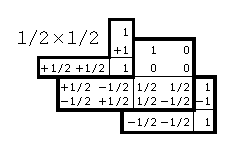
\includegraphics[width=0.28\textwidth]{CGt}
	\caption{The Clebsch-Gordan table for combining two spin-1/2. Source: \url{http://pdg.lbl.gov/2002/clebrpp.pdf}.}
	\label{fig:CGt}
\end{figure}

\section{The Metropolis algorithm}

Let's first briefly introduce what a \emph{Markov chain} is. We call a Markov chain a stochastic process where the transition probability that characterizes the transition between states only depends on the previous step and not from the path to get to such step. We can then write \citep[see][]{Hjorth-Jensen2014}
\begin{equation}
	w_i(t+\delta t)=\sum_j W(j \rightarrow i) w_j (t),
	\label{eq:markov_definition}
\end{equation}
where $w_i(t+\delta t)$ is our PDF -- in our case $|\psi_T(R)|^2$ and $W(j \rightarrow i)$ is the probability of jumping from $j$ to $i$, also called the \emph{transition probability}. We also have
\begin{equation}
	\sum_{i}w_i(t) = 1.
\end{equation}
due to the normalization condition. We can see from equation (\ref{eq:markov_definition}) the probability density function at $t+\delta t$ only depends on its previous state $t$. 

In the case of infinite dimensionality, representing $W$ as a matrix, we have
\begin{equation}
	\hat{w}(t+\delta t) = \hat{W}\hat{w}(t).
\end{equation}
from which
\begin{equation}
	\hat{w}(\infty)= \hat{W} \hat{w}(\infty).
\end{equation}
Then, the problem is just an eigenvalue problem with eigenvalue $1$.

Now, let's consider an \emph{ergodic} system, where the average over time of a process is the same as the ensemble average. Or in other words, as one increases the steps, there exists a positive probability measurement at step $n$ that is independent on the probability distribution at the initial step $0$. It holds
\begin{equation}
	W(i \rightarrow j) w_i= W(j \rightarrow i) w_j,
\end{equation}
from which
\begin{equation}
	R \doteqdot \frac{W(i \rightarrow j)}{W(j \rightarrow i)}=\frac{w_j}{w_i}=\frac{|\psi_T (r^{\text{new}})|^2}{|\psi_T (r^{\text{old}})|^2}.
\end{equation}

Since $W(i \rightarrow j)$ is unknown, we model it as the product of two probabilities:
\begin{equation}
	W(i \rightarrow j)=A(i \rightarrow j) \, T(i \rightarrow j),
\end{equation}
where $A(i \rightarrow j)$ is the probability of accepting the move and $T(i \rightarrow j)$ is the probability of transition from the state $i$ to the state $j$. In a similar way we can write:
\begin{equation}
	W(j \rightarrow i)=A(j \rightarrow i) \, T(j \rightarrow i).
\end{equation}

\subsection{Brute force sampling}
The \emph{brute force} Metropolis algorithm simply consists in the assumption that the transition probability is symmetric, that is
\begin{equation}
	T(i \rightarrow j)= T (j \rightarrow i),
\end{equation}
which leads to
\begin{equation}
	\frac{W(i \rightarrow j )}{W(j \rightarrow i)}=\frac{A(i \rightarrow j )}{A(j \rightarrow i)}.
\end{equation}
Then, we can distinguish between two cases.
\begin{itemize}
	\item If $\dfrac{w_j}{w_i}\geq 1$, then
	\begin{equation}
		A(i \rightarrow j ) \geq A(j \rightarrow i).
	\end{equation}
	So, if we manage to move to such a state, we accept this move because we are moving to a higher probability region.
	\item If $\dfrac{w_j}{w_i} < 1$, then
	\begin{equation}
		A(j \rightarrow i ) > A(i \rightarrow j).
	\end{equation}
	We can't blindly reject this move just because we are moving to a lower probability region, but we can't also accept all of this kind of moves. So, what one does is to compute a random number $r \in (0,1)$ and to accept the move if $r \leq w_j/w_i$.
\end{itemize}
To summarize, one sets
\begin{equation}
	A(i\rightarrow j) 
	= \text{min} \left(1, \frac{w_j}{w_i} \right)
	= \text{min} \left(1, \frac{|\psi_T(r^{\text{new}})|^2}{|\psi_T(r^{\text{old}})|^2} \right)
\end{equation}
and then compares with a random number $r \in (0,1)$. If $A(i\rightarrow j) \geq r$ the step is accepted, otherwise it's rejected.

\subsection{Importance sampling and Schödinger equation as a diffusion problem}
\label{sec:importance}

\emph{Importance sampling} consists in doing more clever assumptions on the shape of $T(i \rightarrow j)$. The discussion is the same as the brute force case, but this time we have to set
\begin{equation}
	A(i\rightarrow j) 
	= \text{min} \left(1, \frac{w_jT(j \rightarrow i)}{w_iT(i \rightarrow j)} \right)
	= \text{min} \left(1, \frac{|\psi_T(r^{\text{new}})|^2T(j \rightarrow i)}{|\psi_T(r^{\text{old}})|^2T(i \rightarrow j)} \right).
	\label{eq:acceptance_imp}
\end{equation}
If we recast the Schr\"{o}dinger equation as a diffusion problem, $T(i \rightarrow j)$ is going to be a Gaussian distribution (or a modified Gaussian); let's do that.

The main idea is to model $T(i \rightarrow j)$ in order to reflect the shape of the trial wave-function itself and have in this way a more ``intelligent'' walk, that wastes less points. The walk is generated using the Fokker-Planck and the Langevin equations; the former -- for a one-dimension diffusion problem -- is
\begin{equation}
	\frac{\partial P}{\partial t} = D \dfrac{\partial}{\partial x} \left( \dfrac{\partial}{\partial x} - F \right)P(x,t),
\end{equation}
where
$P(x,t)$ is the time-dependent probability density, $D$ is the \emph{diffusion coefficient} (it's $0.5$ for the Schr\"{o}dinger equation, see \cite{Hoegberget2013}) and $F$ is the \emph{drift term}.

The Langevin equation, on the other hand, reads as
\begin{equation}
	\frac{\partial x(t)}{\partial t} = DF(x(t)) + \eta,
	\label{eq:langevin}
\end{equation}
being $\eta$ a \emph{random variable}. By solving equation (\ref{eq:langevin}) with Euler's method, it follows that the new position is given by
\begin{equation}
	y = x + DF(x)\Delta t + \xi,
\end{equation}
being $\xi$ a \emph{Gaussian} random variable and $\Delta t$ a chosen time step.

For two or more dimensions, the Fokker-Planck equation is just
\begin{equation}
	\frac{\partial P}{\partial t} = \sum_i D \dfrac{\partial}{\partial \vec{x}_i} \left( \frac{\partial}{\partial \vec{x}_i} - \vec{F}_i \right)P(\vec{x}_i,t)
\end{equation}
We can obtain a convergence to a stationary probability density setting the left hand side to zero, that means all the terms of the sum must be equal to zero. Expanding the product, we obtain
\begin{equation}
	\frac{\partial^2 P}{\partial \vec{x}_i^2} = P \frac{\partial}{\partial \vec{x}_i}\vec{F}_i + \vec{F}_i \frac{\partial}{\partial \vec{x}_i}P.
\end{equation}
Since the drift vector has the form $\vec{F} = g(\vec{x}) \dfrac{\partial P}{\partial \vec{x}}$, we get
\begin{equation}
	\frac{\partial ^2 P}{\partial \vec{x}_i^2 } = P \frac{\partial g}{\partial P} \left( \frac{\partial P}{\partial \vec{x}_i} \right)^2 + Pg \frac{\partial ^2 P}{\partial \vec{x}_i^2} + g \left( \frac{\partial P}{\partial \vec{x}_i} \right)^2.
	\label{eq:intermediate_imp}
\end{equation}

If we want a stationary density the left hand side of equation (\ref{eq:intermediate_imp}) must be zero, and this is possible only if $g = \dfrac{1}{P}$. With this substitution, the drift vector reads as
\begin{equation}
	\vec{F} = \frac{1}{P} \nabla P.
	\label{eq:drift_vector}
\end{equation}
Since -- as we said many times before --  our probability density is the modulus squared of the trial wave-function, that is
\begin{equation}
	P = |\psi_T|^2,
\end{equation}
the drift vector in equation (\ref{eq:drift_vector}) finally reads as
\begin{equation}
	\vec{F} = 2 \frac{1}{\Psi_T} \nabla \Psi_T.
\end{equation}
Written in this way, $\vec{F}$ is also called the \emph{quantum force}. This force pushes the walker in those regions where the trial wave function is larger, increasing the efficiency of the simulation.

Solving the Fokker-Plank equation finally gives an expression for the transition probability $T(x \rightarrow y)$, that turns out can be expressed as the Green function
\begin{equation}
G(y,x, \Delta t) = \dfrac{1}{(4 \pi D \Delta t)^{3N/2}} \exp(-(y - x - D \Delta t F(x))^2 / 4 D \Delta t).
\end{equation}

With this expression, the acceptance ratio in equation (\ref{eq:acceptance_imp}) becomes
\begin{equation}
	R 
	= \frac{|\psi_T(y)|^2T(y \rightarrow x)}{|\psi_T(x)|^2T(x \rightarrow y)}
	= \frac{|\psi_T(y)|^2G(x,y,\Delta t)}{|\psi_T(x)|^2G(y,x,\Delta t)}.
\end{equation}


\subsection{Implementation}

\begin{figure}[h]%[H]
	\centering
	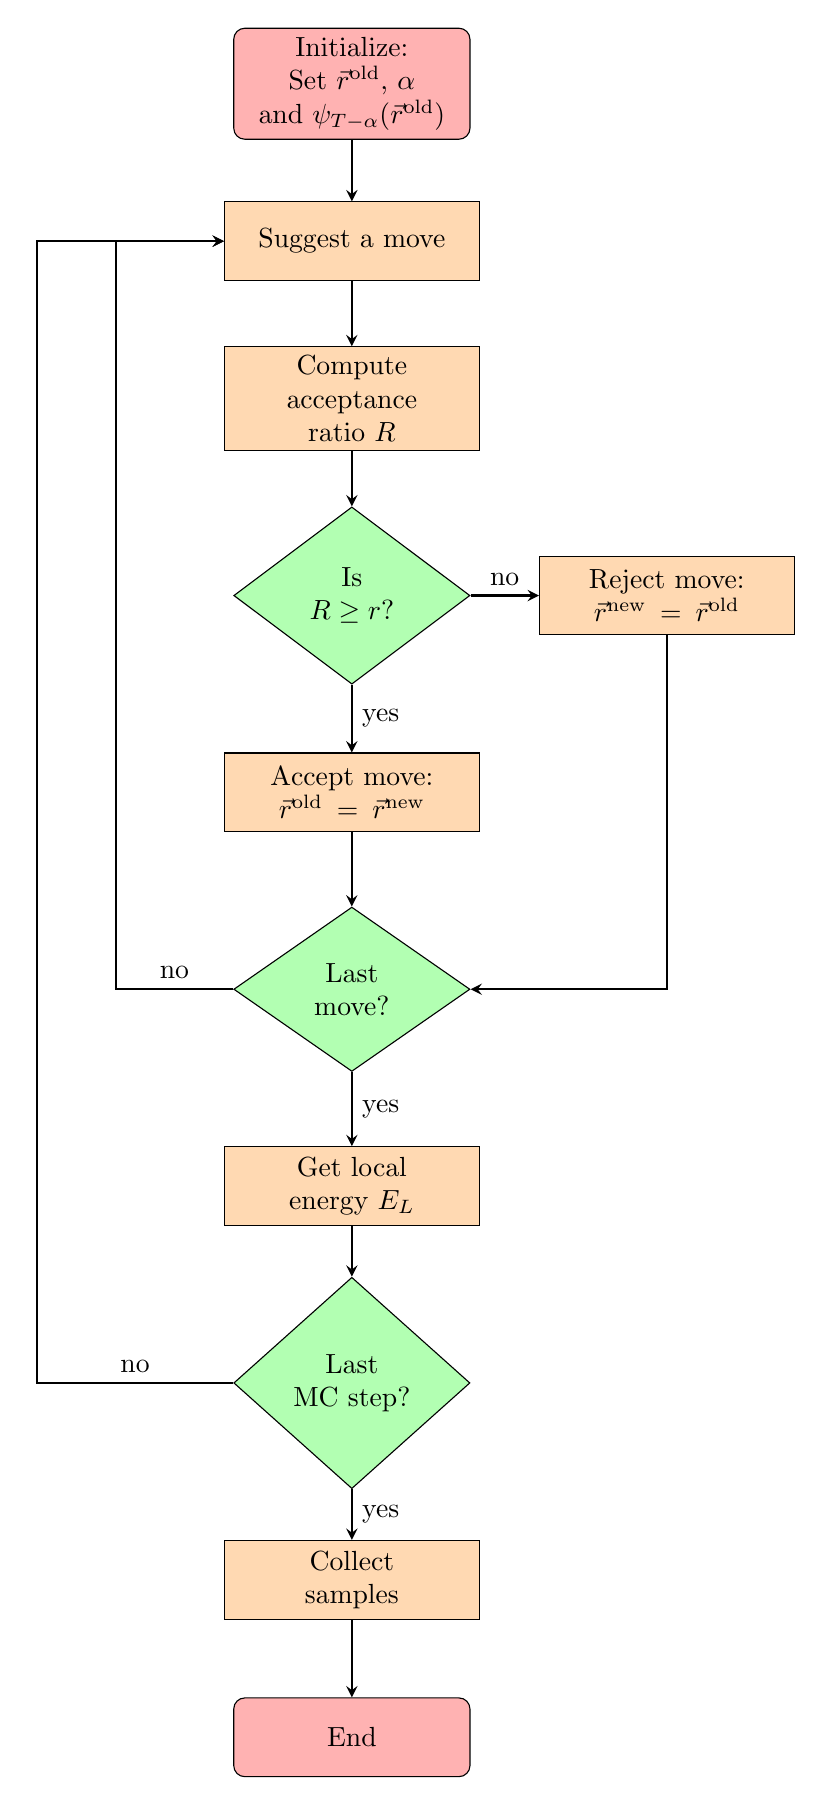
\begin{tikzpicture}[node distance=2cm]
	
		% Draw the nodes
		\node (start) [startstop, align=center] {Initialize:\\ Set $\vec{r}^{\text{old}}$, $\alpha$\\ and $\psi_{T-\alpha}(\vec{r}^{\text{old}})$};
		%\node (in1) [io, below of=start] {Input};
		\node (pro1) [process, below of=start] {Suggest a move};
		\node (pro2) [process, below of=pro1] {Compute\\ acceptance\\ ratio $R$};
		\node (dec1) [decision, below of=pro2, yshift=-0.5cm, align=center] {Is\\$R \geq r$?};
		\node (pro3a) [process, below of=dec1, yshift=-0.5cm, align=center] {Accept move:\\ $\vec{r}^{\text{old}} = \vec{r}^{\text{new}}$};
		\node (pro3b) [process, right of=dec1, xshift=2cm] {Reject move:\\ $\vec{r}^{\text{new}} = \vec{r}^{\text{old}}$};
		\node (dec2) [decision, below of=pro3a, yshift=-0.5cm, align=center] {Last\\ move?};
		\node (dec2left) [left of=dec2, xshift=-1cm] {};
		\node (pro5) [process, below of=dec2, yshift=-0.5cm] {Get local\\ energy $E_L$};
		\node (dec3) [decision, below of=pro5, yshift=-0.5cm, align=center] {Last\\ MC step?};
		\node (dec3left) [left of=dec3, xshift=-2cm] {};
		\node (pro6) [process, below of=dec3, yshift=-0.5cm, align=center] {Collect\\ samples};
%		\node (out1) [io, below of=pro2a] {Output};
		\node (stop) [startstop, below of=pro6] {End};
		
		%Draw the arrows
		\draw [arrow] (start) -- (pro1);
		\draw [arrow] (pro1) -- (pro2);
		\draw [arrow] (pro2) -- (dec1);
		\draw [arrow] (dec1) -- node[anchor=west] {yes} (pro3a);
		\draw [arrow] (dec1) -- node[anchor=south] {no} (pro3b);
		\draw [arrow] (pro3b) |- (dec2);
		\draw [arrow] (pro3a) -- (dec2);
		\draw [arrow] (dec2) -- node[anchor=west] {yes} (pro5);
		\draw [arrow] (dec2) -- node[anchor=south] {no} (dec2left.center) |- (pro1);
		\draw [arrow] (pro5) -- (dec3);
		\draw [arrow] (dec3) -- node[anchor=west] {yes} (pro6);
		\draw [arrow] (dec3) -- node[anchor=south] {no} (dec3left.center) |- (pro1);
		\draw [arrow] (pro6) -- (stop);
	
	\end{tikzpicture}
	\caption{Chart flow for the Quantum Variational Monte Carlo algorithm. Adapted from \cite{Hjorth-Jensen2014}.}
	\label{fig:chart_flow}
\end{figure}

We can sum up the algorithm as follows. Given a random number generator that returns aleatory values in the interval $(0, 1)$ with a uniform (or Gaussian for the importance sampling) distribution, then the Metropolis algorithm consists in these steps.
\begin{itemize}
	\item Chosen a starting point $x_0$ and a step length $l$ (or a time-step $\Delta t$ for the importance sampling), a random number $\varepsilon$ is generated in the interval $(0, 1)$.
	\item The proposed step is $x^{\text{new}}=x^{\text{old}} + l\varepsilon$ (or $x^{\text{new}} = x^{\text{old}} + D\vec{F}(x^{\text{old}})\Delta t + \varepsilon$ for the importance sampling).
	\item The probability ratio $R = \frac{|\psi_T(r^{\text{new}})|^2T(j \rightarrow i)}{|\psi_T(r^{\text{old}})|^2T(i \rightarrow j)}$ is computed.
	\item A new random number $r$ is generated in the interval $(0, 1)$.
	\item If $R \geq r$, the step is accepted and the new position is stored by letting $x^{\text{old}}=x^{\text{new}}$.
	\item If $R < r$, the step is rejected and the new position is discarded by letting $x^{\text{new}}=x^{\text{old}}$.
\end{itemize}
A flow chart of this process is sketched in Figure \ref{fig:chart_flow}.
%%%%%%%%%%%%%%%%%%%%%%%%%%%%%%%%%%%%%%%%%%%%%%%%%%%%%%%%%%%
%                                                         %
% CHAPTER 03:                                             %
% The 2-electrons system                                  %
%                                                         %
% This file is part of a BSc Thesis Project. See the      %
% LICENSE file for more information about licensing.      %
%                                                         %
% Author:     Matteo Seclì <secli.matteo@gmail.com>       %
% A.Y.:       2014/2015                                   %
% URL:        https://github.com/matteosecli/QMC          %
%                                                         %
%%%%%%%%%%%%%%%%%%%%%%%%%%%%%%%%%%%%%%%%%%%%%%%%%%%%%%%%%%%

\graphicspath{{Mainmatter/figures/PNG/}{Mainmatter/figures/PDF/}{Mainmatter/figures/}}

\chapter{The 2-electrons system}

\section{The unperturbed system}
\label{sec:2e_unp}

\begin{figure}[H]
	\centering
	\definecolor{myblue}{rgb}{0,0.447,0.741}	
	\begin{tikzpicture}
		\tikzset{>=latex}
		\draw [ultra thick] (-1,0) -- (1,0) node[midway,below,align=center] {\scriptsize $n_x=0$ \\ \scriptsize $n_y=0$};
		\draw [very thick, myblue, ->] (-0.5,-0.5) -- (-0.5,0.5);
		\draw [very thick, myblue, ->] (0.5,0.5) -- (0.5,-0.5);
	\end{tikzpicture}
	\caption{The 2-electrons system configuration.}
	\label{fig:sketch_2e}
\end{figure}

We will first consider the unperturbed system (without the electron-electron repulsion) with $\omega = 1$, that has Hamiltonian
\begin{equation}
	\hat{H}_0 = 
	\sum_{i=1}^{N} \left( -\frac{1}{2}\nabla_i^2 + \frac{1}{2}\omega^2r_i^2 \right),
\end{equation}
with $N=2$ and in two dimensions. For a single electron in a two-dimensional (isotropic) harmonic oscillator, the energy is $E_s = \hbar\omega(n_x + n_y + 1)$, where $n_x$ and $n_y$ are the quantum numbers for the $x$ and $y$ dimensions. The ground state (see Figure \ref{fig:sketch_2e}) is obtained for $(n_x,n_y) = (0,0)$ which gives $E_s = \SI{1}{\atomicunit}$. Since we have two particles, the ground state energy of our system is in total
\begin{equation*}
	E_{\text{gs}} = \SI{2}{\atomicunit}.
\end{equation*}
In general, for $\omega \neq 1$, the energy will just be $E_{\text{gs}} = 2\omega$.

Now, we have to choose a trial wave-function. For a single electron, the exact wave-function of the ground state is
\begin{equation}
	\phi_{n_x,n_y}(x, y) = A H_{n_x}(\sqrt{\omega}x)H_{n_y}(\sqrt{\omega}y)\exp\left(-\omega\left(x^2 + y^2\right)/2\right),
	\label{eq:phi_qnums}
\end{equation}
being $A$ a normalization constant and $H_n$ is the (physical) Hermite polynomial of order $n$. Since the 0-th order Hermite polynomials are just $1$ and the two-particles wave-function can be seen as a product of the single-particle wave-functions, our total wave-function will just be
\begin{equation}
	\phi(\vec{r}_1,\vec{r}_2) = C \exp\left(-\omega\left(r_1^2 + r_2^2\right)/2\right).
	\label{eq:two_part_noint_solution}
\end{equation}
Adding a variational parameter $\alpha$ and forgetting about the normalization constant $C$, we obtain our trial wave-function for this case:
\begin{equation}
	\psi_T(\vec{r}_1,\vec{r}_2) = \exp\left(-\alpha\omega\left(r_1^2 + r_2^2\right)/2\right).
\end{equation}
Note that, since the correct solution of this problem is equation (\ref{eq:two_part_noint_solution}), we expect to obtain a variational energy \emph{exactly} equal to 2 for $\alpha = 1$.

\begin{figure}[H]
	\centering
	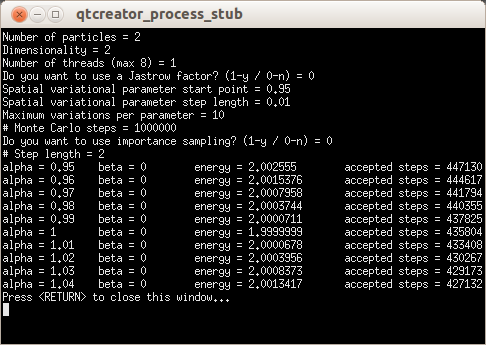
\includegraphics[width=0.45\textwidth]{two-part-non-int}
	\caption{The program running for a two-electron system without repulsion.}
	\label{fig:run_window_2e_no_rep}
\end{figure}

The electron-electron repulsion can be simply turned off by commenting out the line
\begin{lstlisting}[language=cpp]
	MySystem.add_potential(new eRepulsion(gP));
\end{lstlisting}
in the code. Running the program in Qt Creator shows the window in Figure \ref{fig:run_window_2e_no_rep}, where some parameters can be specified before the actual calculation begins.

Just using a finer step for $\alpha$, we obtain the energy graph shown in Figure \ref{fig:2e_no_rep}.
\begin{figure}[h]%[H]
	\centering
	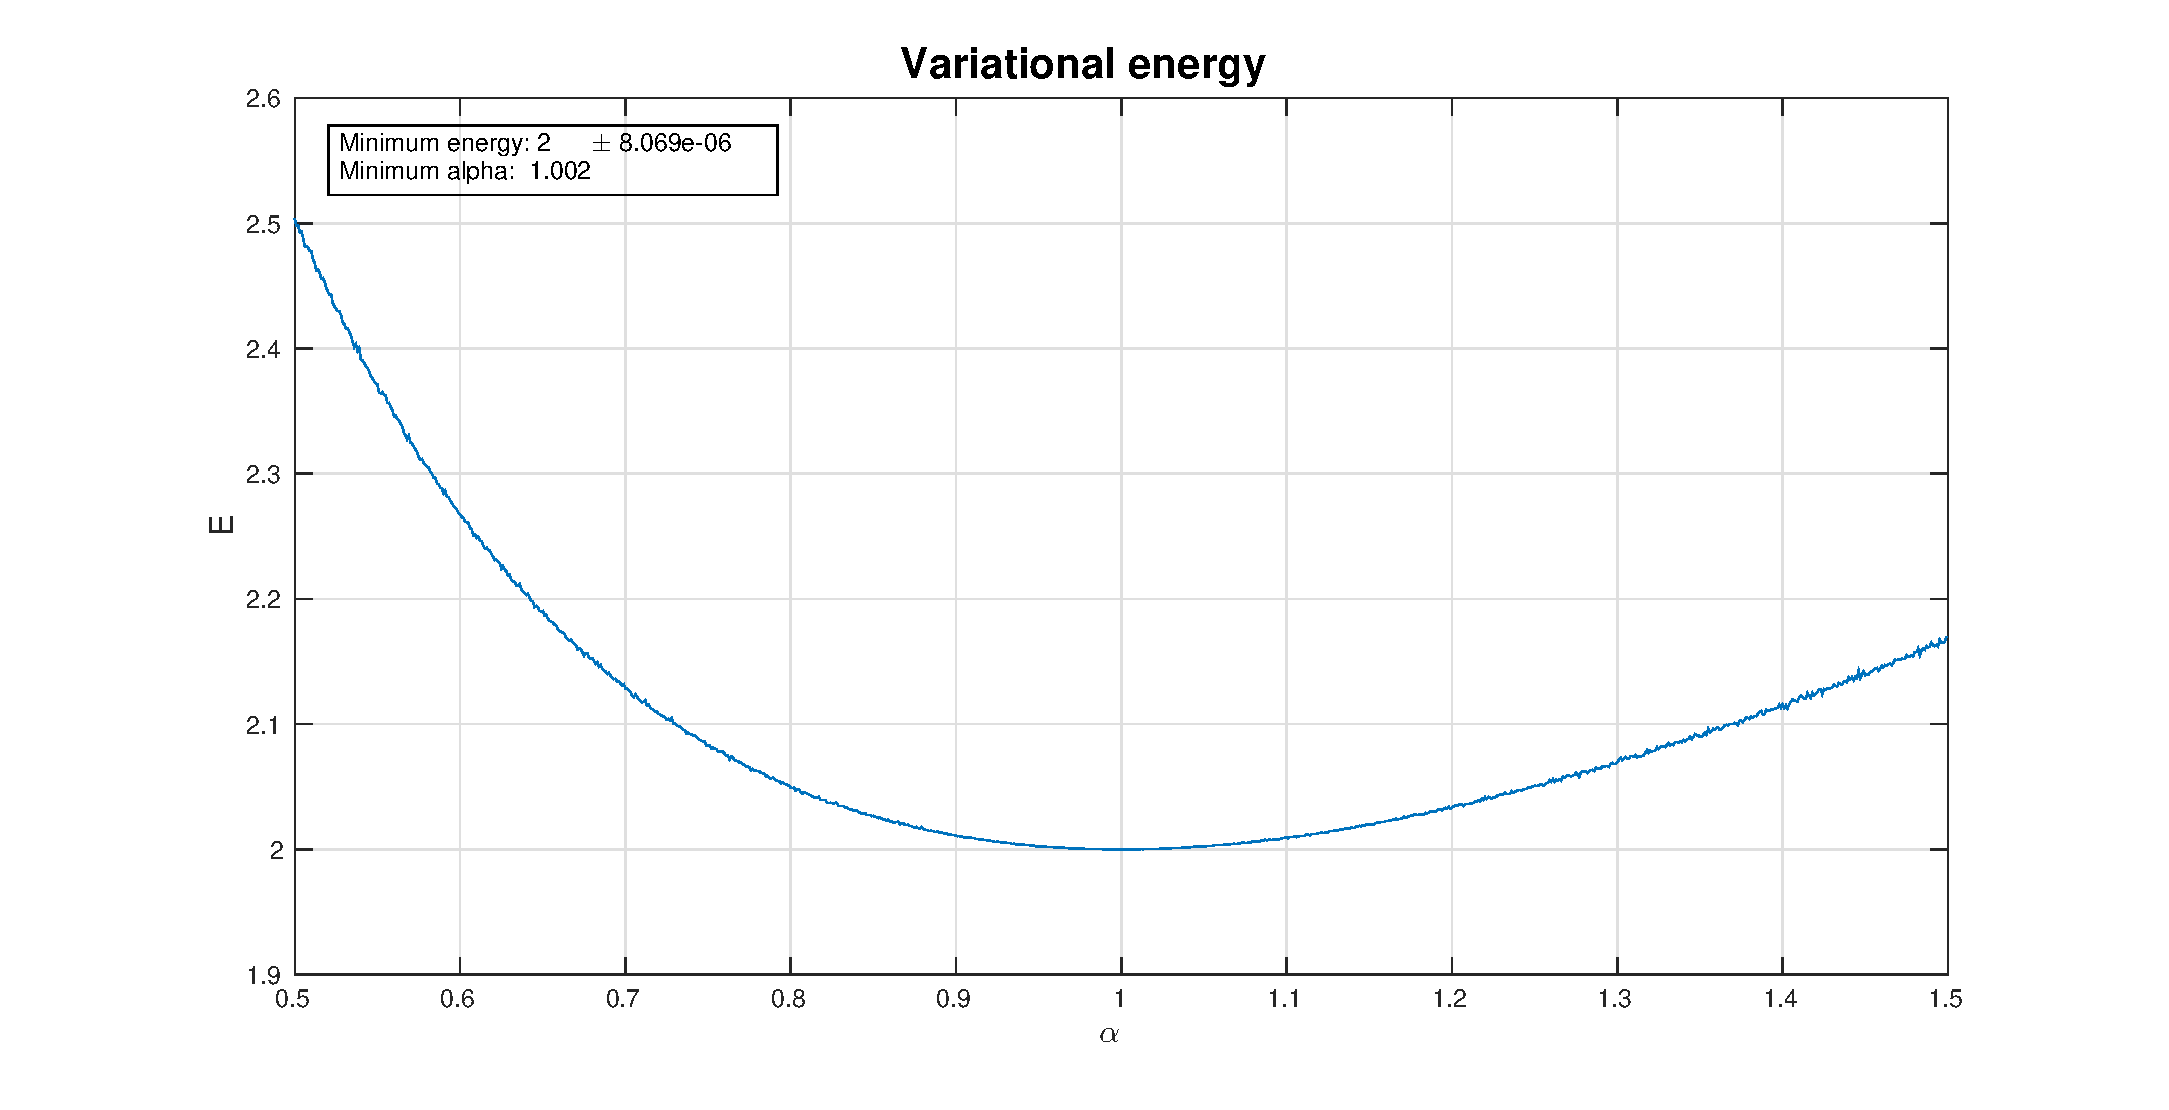
\includegraphics[width=\textwidth]{2e-norep}
	\caption{The variational energy versus the variational parameter $\alpha$. The settings used are: brute force sampling with step length 2, no Jastrow factor, no parallelization, $1000$ variations of $\alpha$ around $1$ with step $0.001$, $\SI{1e7}{}$ Monte Carlo steps. Acceptance ratio varies from $40$ to $\SI{60}{\percent}$.}
	\label{fig:2e_no_rep}
\end{figure}

As you can see in Figure \ref{fig:2e_no_rep}, we get $E_{\text{gs}} = 2$ with a high degree of precision for $\alpha=1$\footnote{Actually the minimum is for $\alpha=1.002$, but in this case we are not using so many steps that we can trust the third decimal digit. The smaller $\alpha$-step was just used to have a nicer plot.}.

We can also state that the total spin (better: its $z$-component) of the system is 0, as shown in equation (\ref{eq:total_spin}). If you want a more ``physical'' reason than just reading off a table of coefficients, this is a direct consequence of the shape of the wave-function for a fermionic system, as shown in equation (\ref{eq:slater_example}). In fact, in our case the spatial part of the two single-particle wave-functions is equal (they occupy the same energy level), yielding to
\begin{equation}
	\Ket{1} = \Ket{\phi}\otimes\Ket{\chi_1},
	\qquad
	\Ket{2} = \Ket{\phi}\otimes\Ket{\chi_2}.
\end{equation}
Comparing with equation (\ref{eq:identical_particles}) one sees that $\Ket{\psi} = 0$ unless $\Ket{1} \neq \Ket{2}$, and since the spatial parts are equal one has to conclude that $\Ket{\chi_1} \neq \Ket{\chi_2}$\footnote{We don't want $\Ket{\psi} = 0$ because it's not a physical state and it is not normalizable.}. Now, 
\begin{equation}
	\Ket{\chi_1} = \Ket{s,m_s}
\end{equation}
with $s=1/2$, so we have to say that -- for example -- particle 1 has spin-up ($m_s=1/2$) and particle 2 has spin-down ($m_s=-1/2$). This fact is also known as the \emph{Pauli exclusion principle}, and applies for a generic system of fermions.

\section{The complete system}
We want now to analyse the system with the full Hamiltonian, namely the Hamiltonian in equation (\ref{eq:full_hamiltonian}):
\begin{equation}
	\hat{H}=-\frac{1}{2} \nabla^2_1 - \frac{1}{2} \nabla^2_2+\frac{1}{2}\omega r_1^2+\frac{1}{2}\omega r_2^2+ \frac{1}{|\vec{r_1}-\vec{r_2}|},
\end{equation}
where $\vec{r_1}$ and $\vec{r_2}$ are the position operators of the two particles.

You see that this time we have a problem when two particles are very near to each other, since the term
\begin{equation*}
	\sum_{i<j}\frac{1}{|\vec{r_1}-\vec{r_2}|}
\end{equation*}
tends to be a division by zero. Introducing the substitution
\begin{equation}
\begin{cases}
\vec{r}=\vec{r_1}-\vec{r_2} \\ 
\vec{R}=\frac{1}{2}(\vec{r_1}+\vec{r_2}) 
\end{cases}
\end{equation}
the Hamiltonian can be rewritten in a decoupled way as \citep[see][]{Taut1993}
\begin{equation}
    \hat{H} = -\nabla_{\vec{r}}^2 - \frac{1}{4}\nabla_{\vec{R}}^2 - \frac{1}{4}\omega^2\vec{r}^2 + \omega^2\vec{R}^2 + \frac{1}{r}.
\end{equation}
Since the Hamiltonian is spin-independent, we can factorize the wave-function as
\begin{equation}
    \psi(\vec{r},\vec{R},m_{s_1},m_{s_2}) = \varphi(\vec{r})\xi(\vec{R})\chi(m_{s_1},m_{s_2})
\end{equation}
which separates the Schr\"{o}dinger equation into
\begin{equation}
    \left( -\frac{1}{2}\nabla_{\vec{r}}^2 + \frac{1}{2}\omega_r^2\vec{r}^2 + \frac{1}{2}\frac{1}{r} \right)\varphi(\vec{r}) = E_r\varphi(\vec{r})
    \label{eq:Seq_relative_distance}
\end{equation}
and
\begin{equation}
    \left( -\frac{1}{2}\nabla_{\vec{R}}^2 + \frac{1}{2}\omega_R^2\vec{R}^2 \right)\xi(\vec{R}) = E_R\xi(\vec{R}),
\end{equation}
where $\omega_r = \frac{1}{2}\omega$ and $\omega_R = 2\omega$.

We are not interested in the $R$-part of the solution, since it gives no troubles; we are more interested in equation \eqref{eq:Seq_relative_distance}, because we can cancel the divergence for $r \to 0$ working on the solution. We can also forget about the harmonic potential because it gives no divergence. Since we are only interested in the radial part of the solution, the relevant contributions from the laplacian in spherical coordinates are
\begin{equation}
    \nabla^2_r = \frac{d^2}{dr^2} + \frac{1}{r}\frac{d}{dr}.
\end{equation}
We also notice that $\frac{d^2}{dr^2}$ gives a finite contribution (is just the momentum part) and so does $\frac{d}{dr}$. The only piece that is not finite is the $\frac{1}{r}$ in front of $\frac{d}{dr}$, that we can use to cancel the divergence in the interaction potential. Using these facts, equation \eqref{eq:Seq_relative_distance} can be rewritten in a way that is called the \emph{cusp condition} for this system, namely
\begin{equation}
    \lim_{r \to 0} \frac{1}{\varphi(r)}\left( -\cancel{\frac{1}{2}\frac{1}{r}}\frac{d}{dr} + \cancel{\frac{1}{2}\frac{1}{r}} \right)\varphi(r) = 0.
\end{equation}
Solving for $\varphi$ by partial integration gives
\begin{equation}
    \varphi(r) = \exp(Cr),
    \qquad\qquad
    r \to 0
    \label{eq:cusp_solution}
\end{equation}
where $C$ is a constant. For these types of Monte Carlo calculations, a so-called \emph{Padé-Jastrow} factor that has the property \eqref{eq:cusp_solution} is often used. This factor has the form (for two electrons)
\begin{equation}
    \exp\left( \frac{ar}{(1+\beta r)} \right),
\end{equation}
where (in 2 dimensions)
\begin{equation}
    a = 
    \begin{cases}
    1 & \text{anti-parallel spin} \\
    1/3 & \text{parallel spin}
    \end{cases}
\end{equation}
and $\beta$ is a variational parameter. With this factor, our trial wave-function reads as
\begin{equation}
    \psi_T(\vec{r_1},\vec{r_2}) = \exp\left(-\alpha\omega\left(r_1^2 + r_2^2\right)/2\right)\exp\left( \frac{ar}{(1+\beta r)} \right).
    \label{eq:wf_2e}
\end{equation}

Using the ansatz in equation \eqref{eq:wf_2e} in our program, we obtain a preliminary result shown in Figure \ref{fig:2e_rep}.

\begin{figure}[h]%[H]
	\centering
	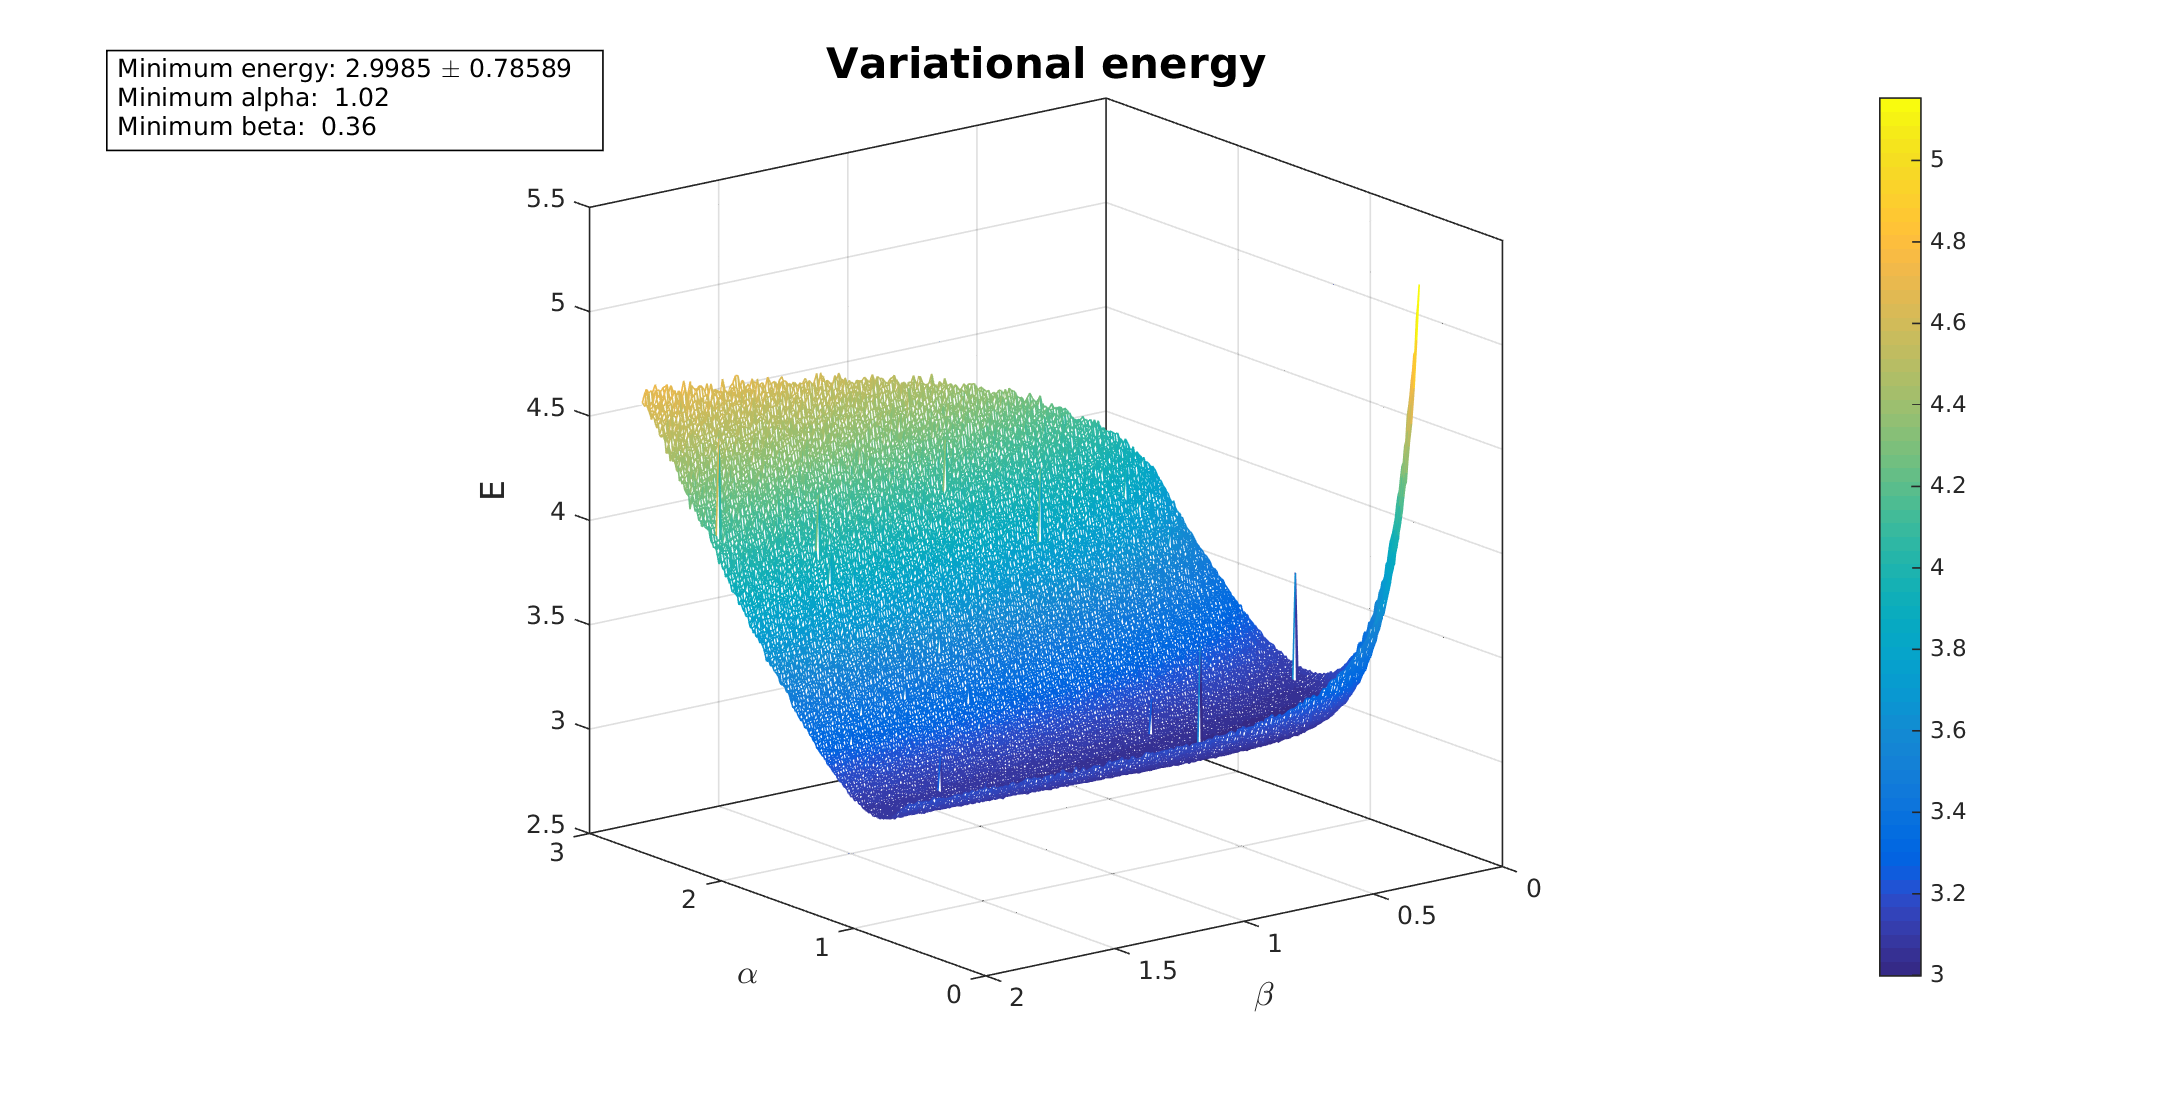
\includegraphics[width=\textwidth]{2e-rep}
	\caption{The variational energy versus the variational parameters $\alpha$ and $\beta$. The settings used are: brute force sampling with step length 2, Jastrow factor, no parallelization, $200$ variations of $\alpha$ and $\beta$ with step $0.01$, $\SI{1e5}{}$ Monte Carlo steps. Acceptance ratio varies from $45$ to $\SI{55}{\percent}$.}
	\label{fig:2e_rep}
\end{figure}

Refining around the minimum value to have better results, we finally obtain the plot in Figure \ref{fig:2e_rep_fine}.

You see that we are very near to the exact result $E_{\text{gs}} = \SI{3}{\atomicunit}$ calculated from \cite{Taut1993} and reported in \cite{PedersenLohne2011}. However, the energy error is still quite big; a way to improve the precision of our program is to \emph{parallelize} it.

\begin{figure}[H]
	\centering
	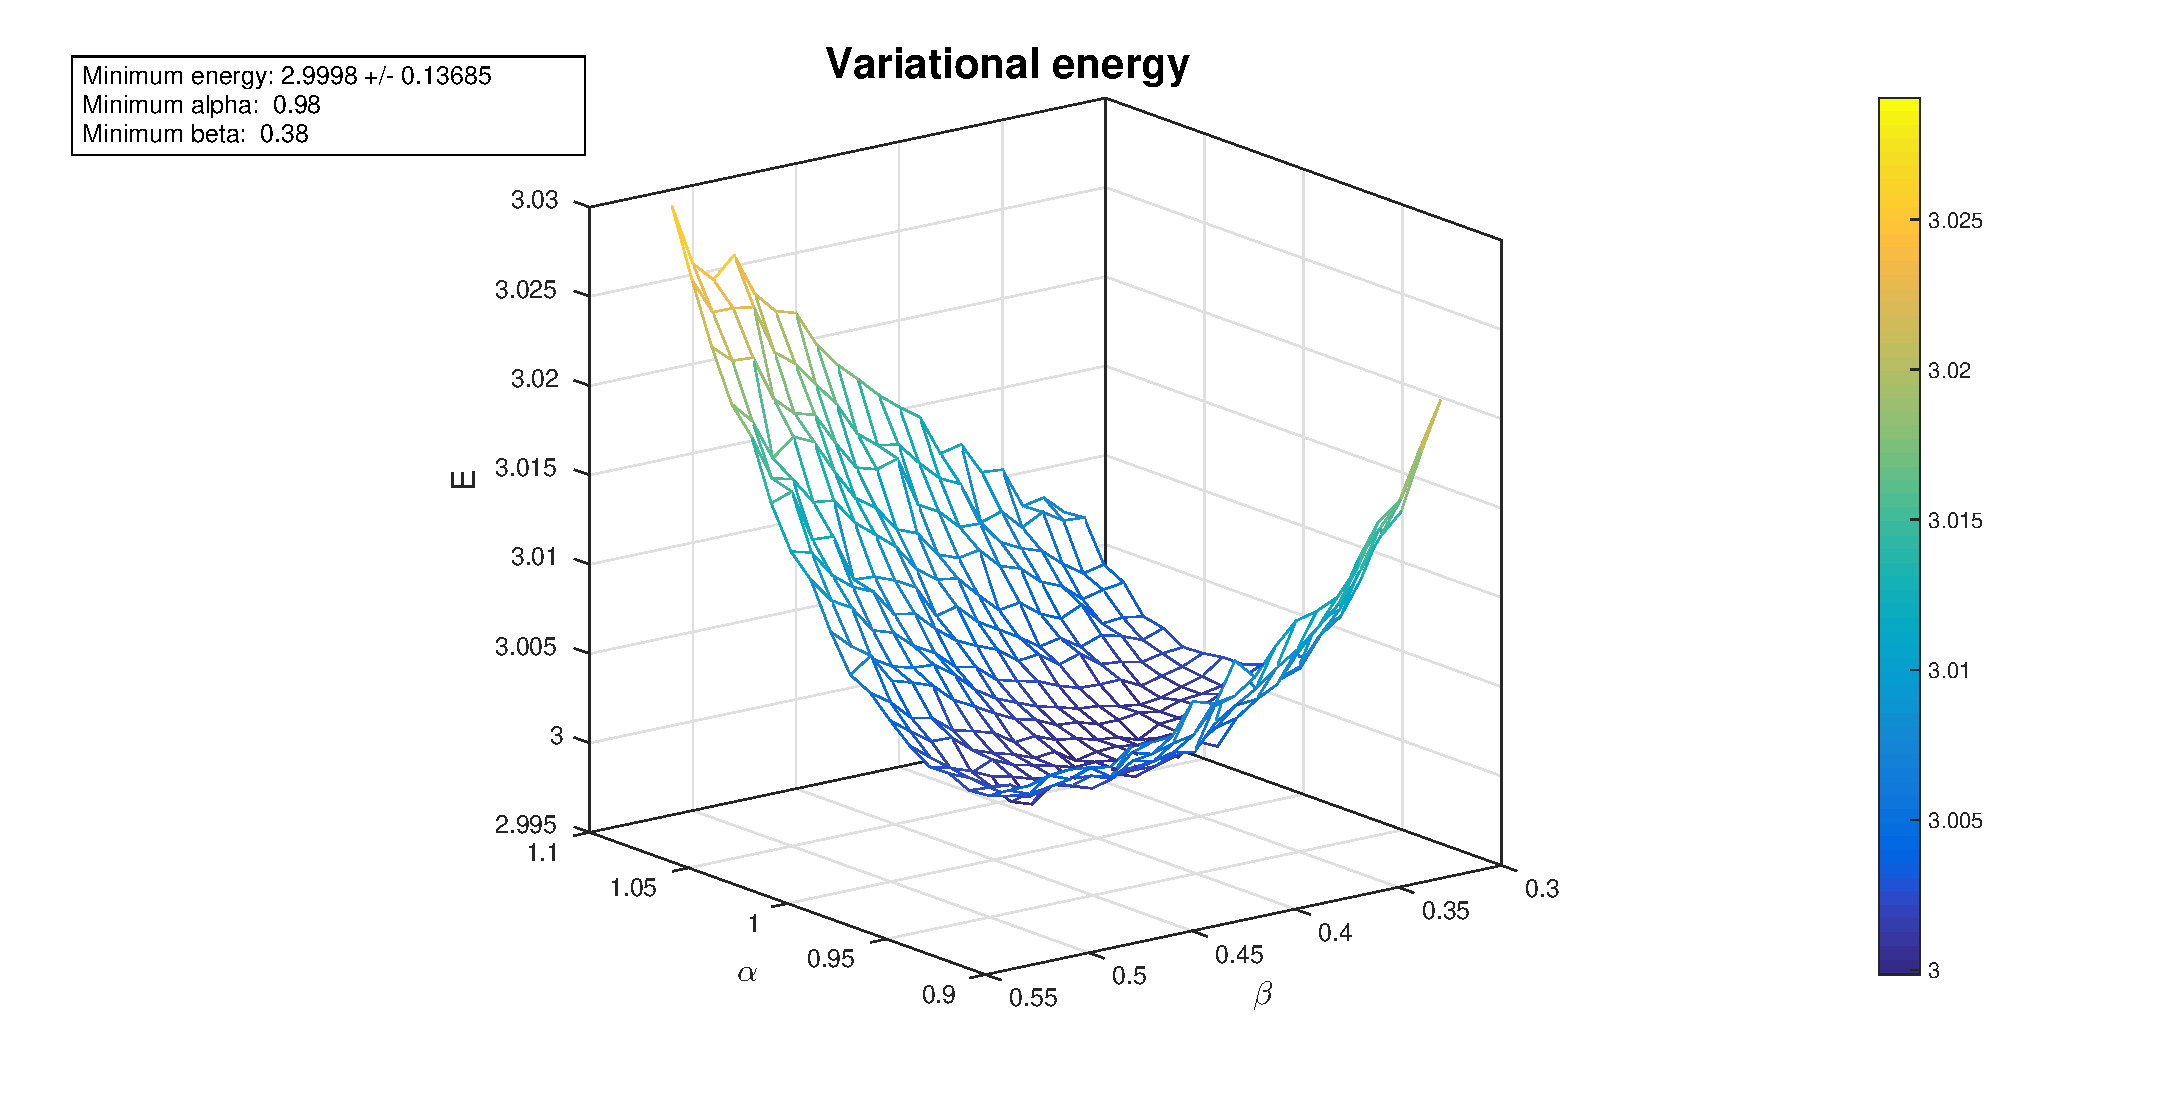
\includegraphics[width=\textwidth]{2e-rep_fine}
	\caption{The variational energy versus the variational parameters $\alpha$ and $\beta$. The settings used are: brute force sampling with step length 2, Jastrow factor, no parallelization, $20$ variations of $\alpha$ and $\beta$ with step $0.01$, $\SI{1e6}{}$ Monte Carlo steps. Acceptance ratio varies from $45$ to $\SI{55}{\percent}$. The relative distance is about $\SI{1.64}{}$ in natural units.}
	\label{fig:2e_rep_fine}
\end{figure}

\subsection{Parallelization}

In this project, parallelization is done by using OpenMP\footnote{\url{http://openmp.org/}.}. The main idea is to run multiple computations of $E_T$ for the same pair of variational parameters $(\alpha,\beta)$ and then take the mean. Since the ``measurements'' of $E_T$ are not correlated, the error on its mean value falls like $1/\sqrt{n}$, where $n$ is the number of measurements. To be sure that the measurements are not correlated we have to make \emph{private} local copies of the variables used in the computation, one for each thread used. Then, we have to sync all the threads in order to be sure that all the measurements are complete, and finally we can take the mean. An example of how this is implemented in our program is given below:

\begin{lstlisting}[language=cpp]
    // Begin parallelization
    omp_set_num_threads(gP.num_threads);
    #pragma omp parallel shared(cumulative_e, cumulative_e2)
    {
        // Make a private copy of all the stuff
        mat cumulative_e_local = zeros<mat>(vmcParams.max_variations+1,vmcParams.max_variations+1);
        mat cumulative_e2_local = zeros<mat>(vmcParams.max_variations+1,vmcParams.max_variations+1);
        struct GeneralParams gP_local = gP;
        struct VariationalParams vP_local = vP;
        struct VMCparams vmcParams_local = vmcParams;

        // Build the orbitals
        Orbitals* MyWaveFunction_local = new AlphaHarmonicOscillator(gP_local, vP_local);

        // Set up the Jastrow factor
        Jastrow* MyJastrowFactor_local;
        if (vmcParams_local.jF_active) MyJastrowFactor_local = new Pade_Jastrow(gP,vP);
        else MyJastrowFactor_local = new No_Jastrow();

        // Make a local copy of the system for convenience
        System MySystem_local = MySystem;

        // Do the mc sampling
        mc_sampling(gP_local, vP_local, vmcParams_local,
                    cumulative_e_local, cumulative_e2_local,
                    MySystem_local, MyWaveFunction_local, MyJastrowFactor_local);

        // Be sure to have all the contributions
        #pragma omp barrier
        #pragma omp critical
        {
            // Add the contributions
            cumulative_e += cumulative_e_local;
            cumulative_e2 += cumulative_e2_local;
        }
    }

    // Normalize to the number of threads
    cumulative_e = cumulative_e/((double) gP.num_threads);
    cumulative_e2 = cumulative_e2/((double) gP.num_threads);
\end{lstlisting}

Re-doing the calculations using parallelization gives the result in Figure \ref{fig:2e_rep_parallel}.
\begin{figure}[H]
	\centering
	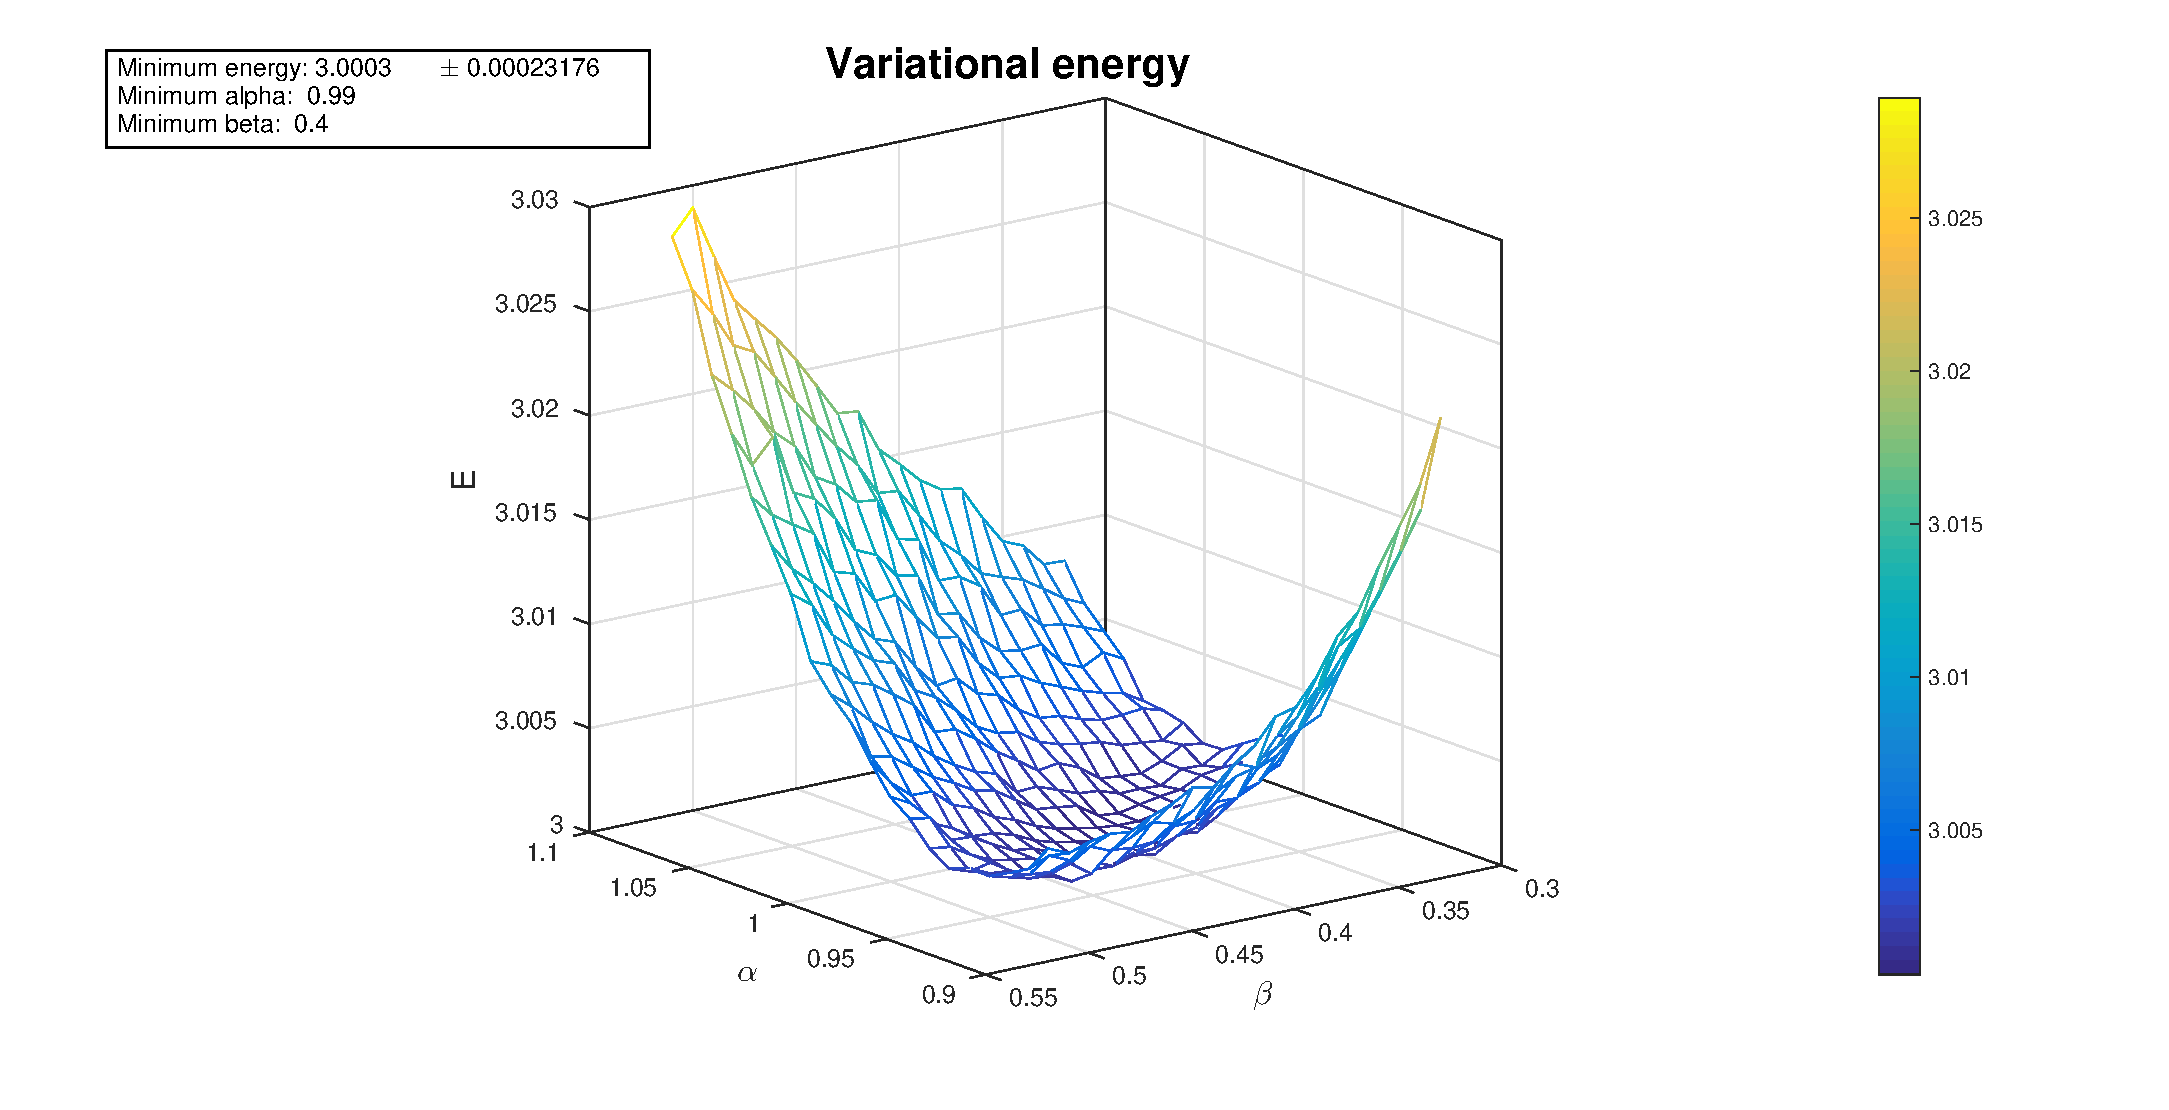
\includegraphics[width=\textwidth]{2e-rep_parallel}
	\caption{The variational energy versus the variational parameters $\alpha$ and $\beta$. The settings used are: brute force sampling with step length 2, Jastrow factor, parallelization (8 threads), $20$ variations of $\alpha$ and $\beta$ with step $0.01$, $\SI{2e5}{}$ Monte Carlo steps. Acceptance ratio varies from $45$ to $\SI{55}{\percent}$.}
	\label{fig:2e_rep_parallel}
\end{figure}
Note that this time, even using a lower number of Monte Carlo steps, we have an amazingly precise estimate for our energy, comparable with the one obtained in \cite{PedersenLohne2011} using Diffusion Monte Carlo.

\subsection{Importance sampling}
Let's now try to implement importance sampling, as explained in Section \ref{sec:importance}. In order to show the differences with the brute force algorithm, we will repeat the calculations with exactly the same settings used in Figure \ref{fig:2e_rep_parallel}, this time with importance sampling active. We will also try to do the calculations for different time-steps $\Delta t = 0.001,\,0.01,\,0.1$.

The results are shown in Figures \ref{fig:2e-rep_imp_small}, \ref{fig:2e-rep_imp_med} and \ref{fig:2e-rep_imp_high}.

As you see, there is a huge difference between the result obtained with $\Delta t = 0.001$ and the one obtained with $\Delta t = 0.1$. This is because, if the time step is too small and we don't have enough Monte Carlo steps, our walker cannot span completely the integration space. It will remain near its starting point and all the points reached will be inside the integration space, close to each other. In fact, the acceptance ratio for the case $\Delta t = 0.001$ and $\Delta t = 0.01$ is \emph{practically} $\SI{100}{\percent}$. The third case, for $\Delta t = 0.1$, has a little lower acceptance ratio, that is about $\SI{99.79}{\percent}$. This fact guarantees that our walker is reaching all the borders of our integration space, and in fact it also reaches some points outside it. In other words, for the given number of Monte Carlo iterations, we have a time-step large enough to cover all the space. If one wants to use a lower time-step to have better precision, he has to increase the number of Monte Carlo cycles; as an example, for $\Delta t = 0.001$, one has to use at least $\SI{1e9}{}$ Monte Carlo loops.

\begin{figure}[H]
	\centering
	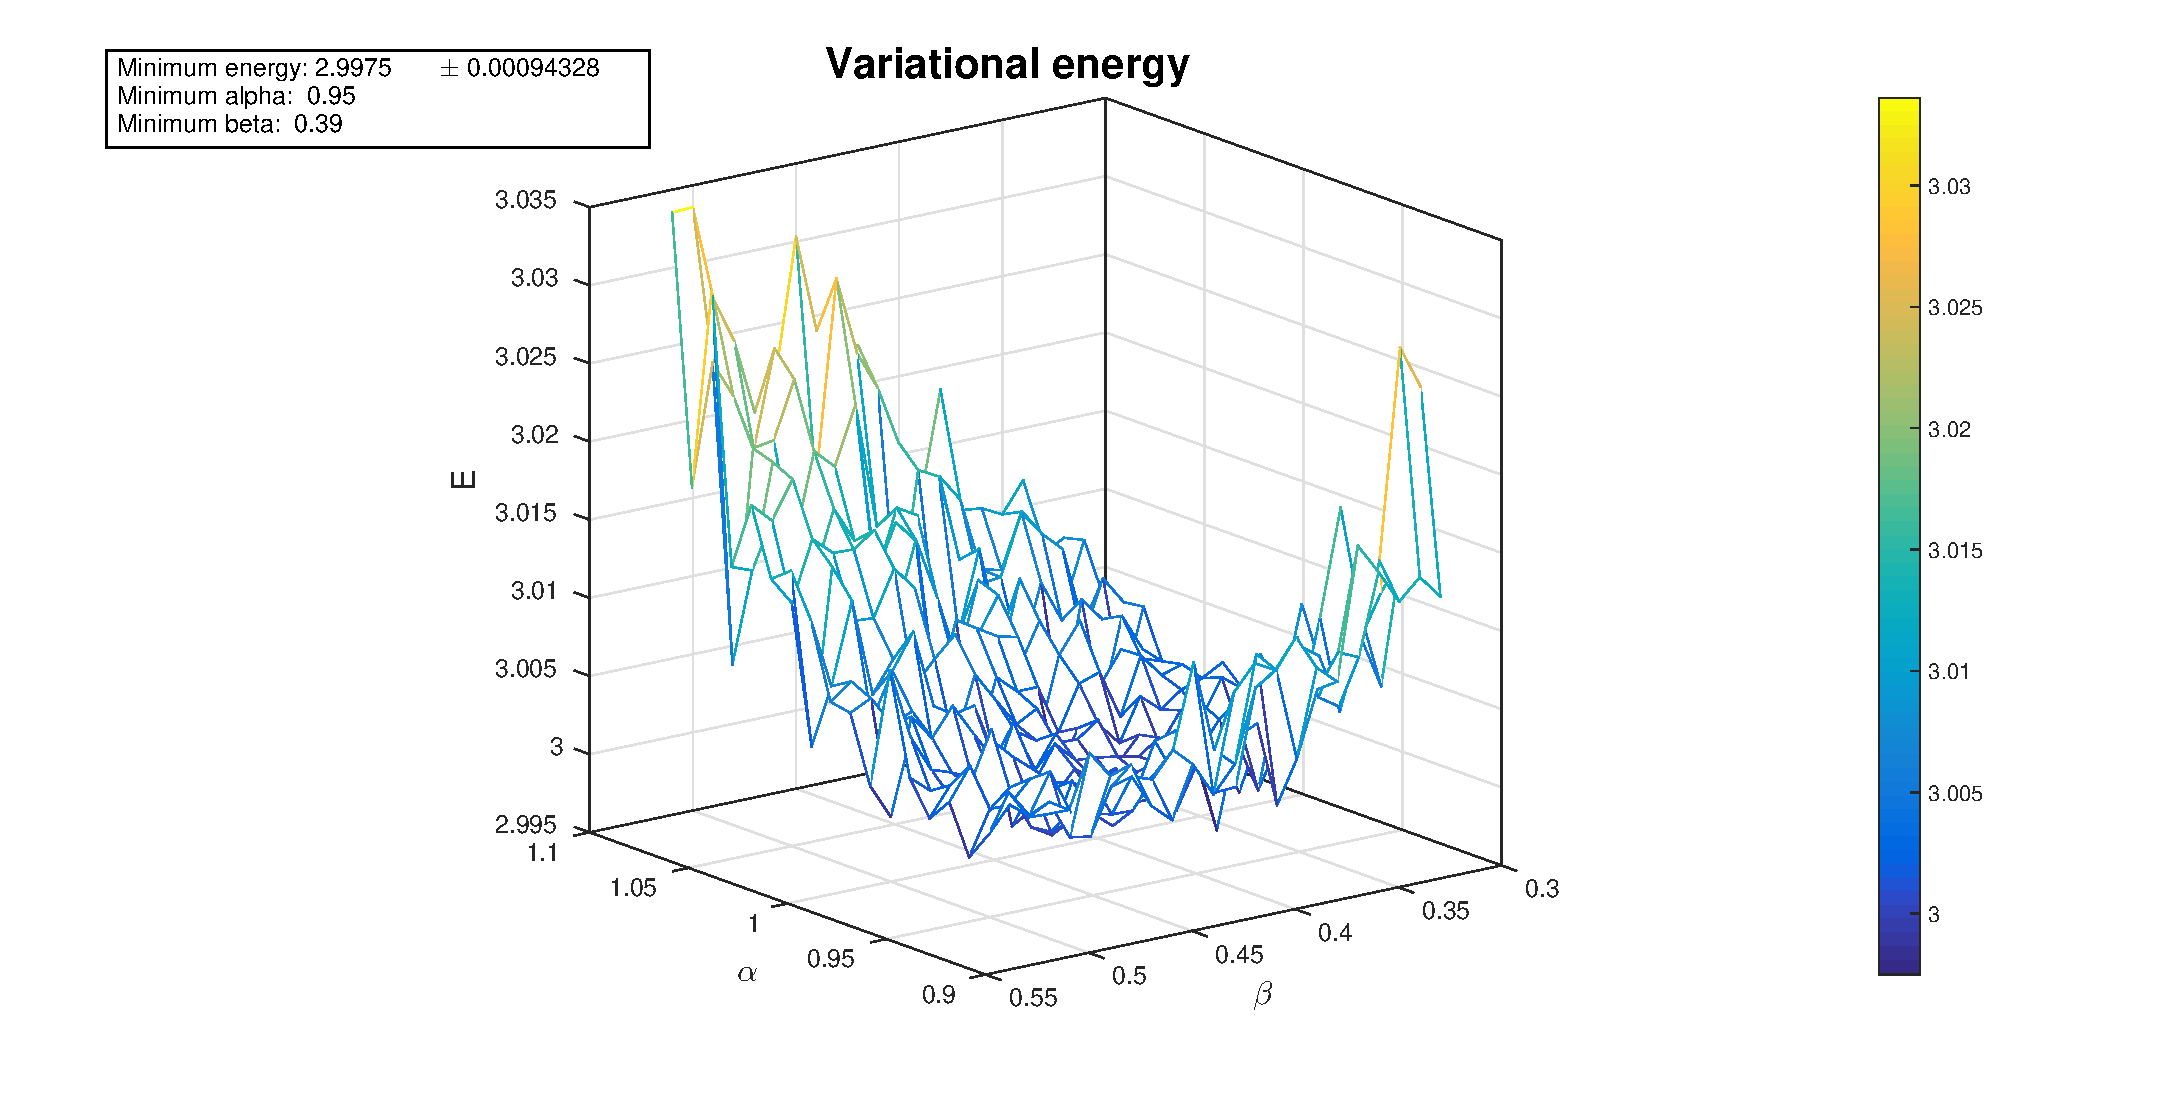
\includegraphics[width=\textwidth]{2e-rep_imp_small}
	\caption{The variational energy versus the variational parameters $\alpha$ and $\beta$. The settings used are: importance sampling with $\Delta t = 0.001$, Jastrow factor, parallelization (8 threads), $20$ variations of $\alpha$ and $\beta$ with step $0.01$, $\SI{2e5}{}$ Monte Carlo steps. Acceptance ratio is about $\SI{99.999}{\percent}$.}
	\label{fig:2e-rep_imp_small}
\end{figure}
\begin{figure}[H]
	\centering
	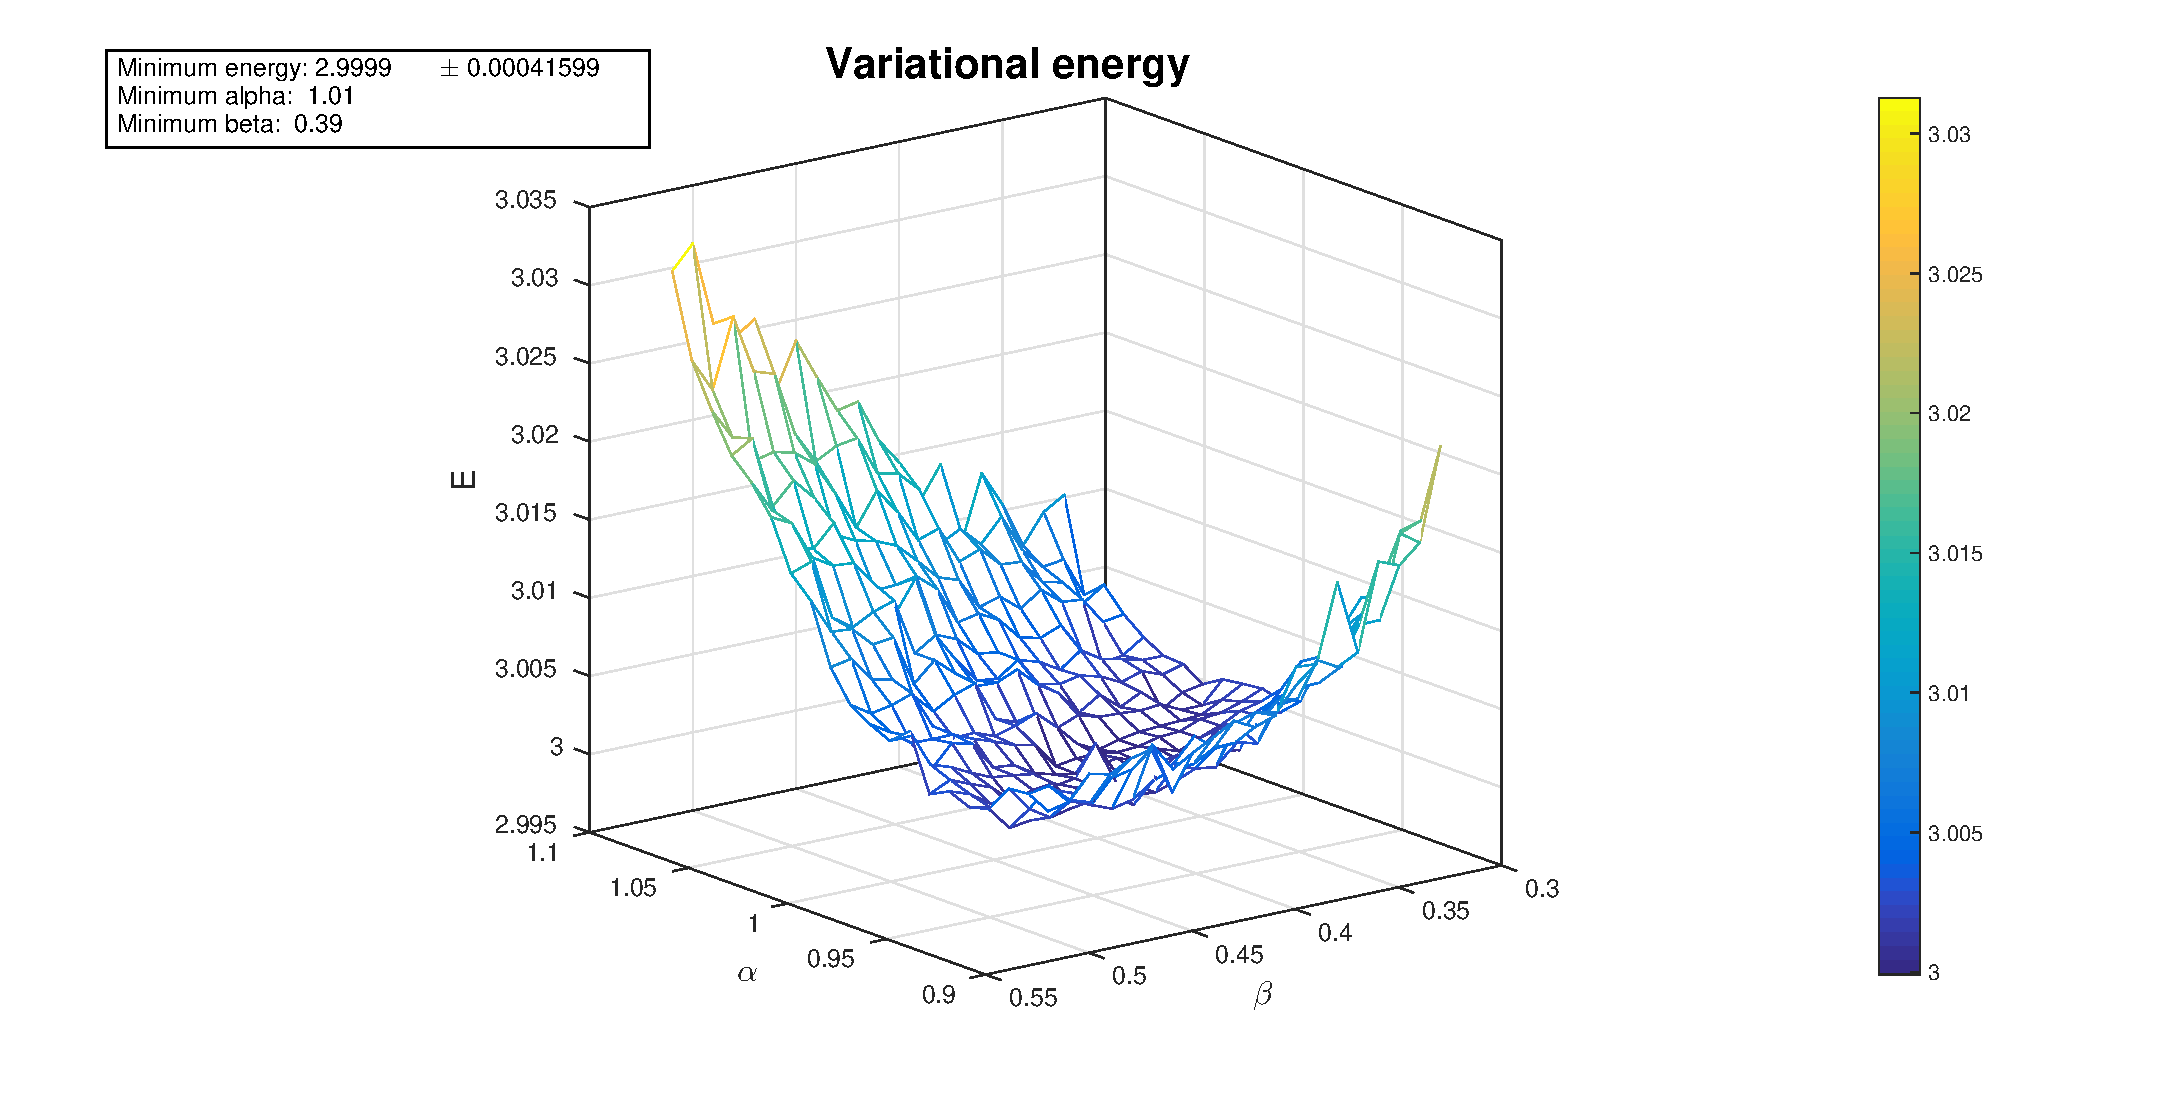
\includegraphics[width=\textwidth]{2e-rep_imp_med}
	\caption{The variational energy versus the variational parameters $\alpha$ and $\beta$. The settings used are: importance sampling with $\Delta t = 0.01$, Jastrow factor, parallelization (8 threads), $20$ variations of $\alpha$ and $\beta$ with step $0.01$, $\SI{2e5}{}$ Monte Carlo steps. Acceptance ratio is about $\SI{99.999}{\percent}$.}
	\label{fig:2e-rep_imp_med}
\end{figure}
\begin{figure}[H]
	\centering
	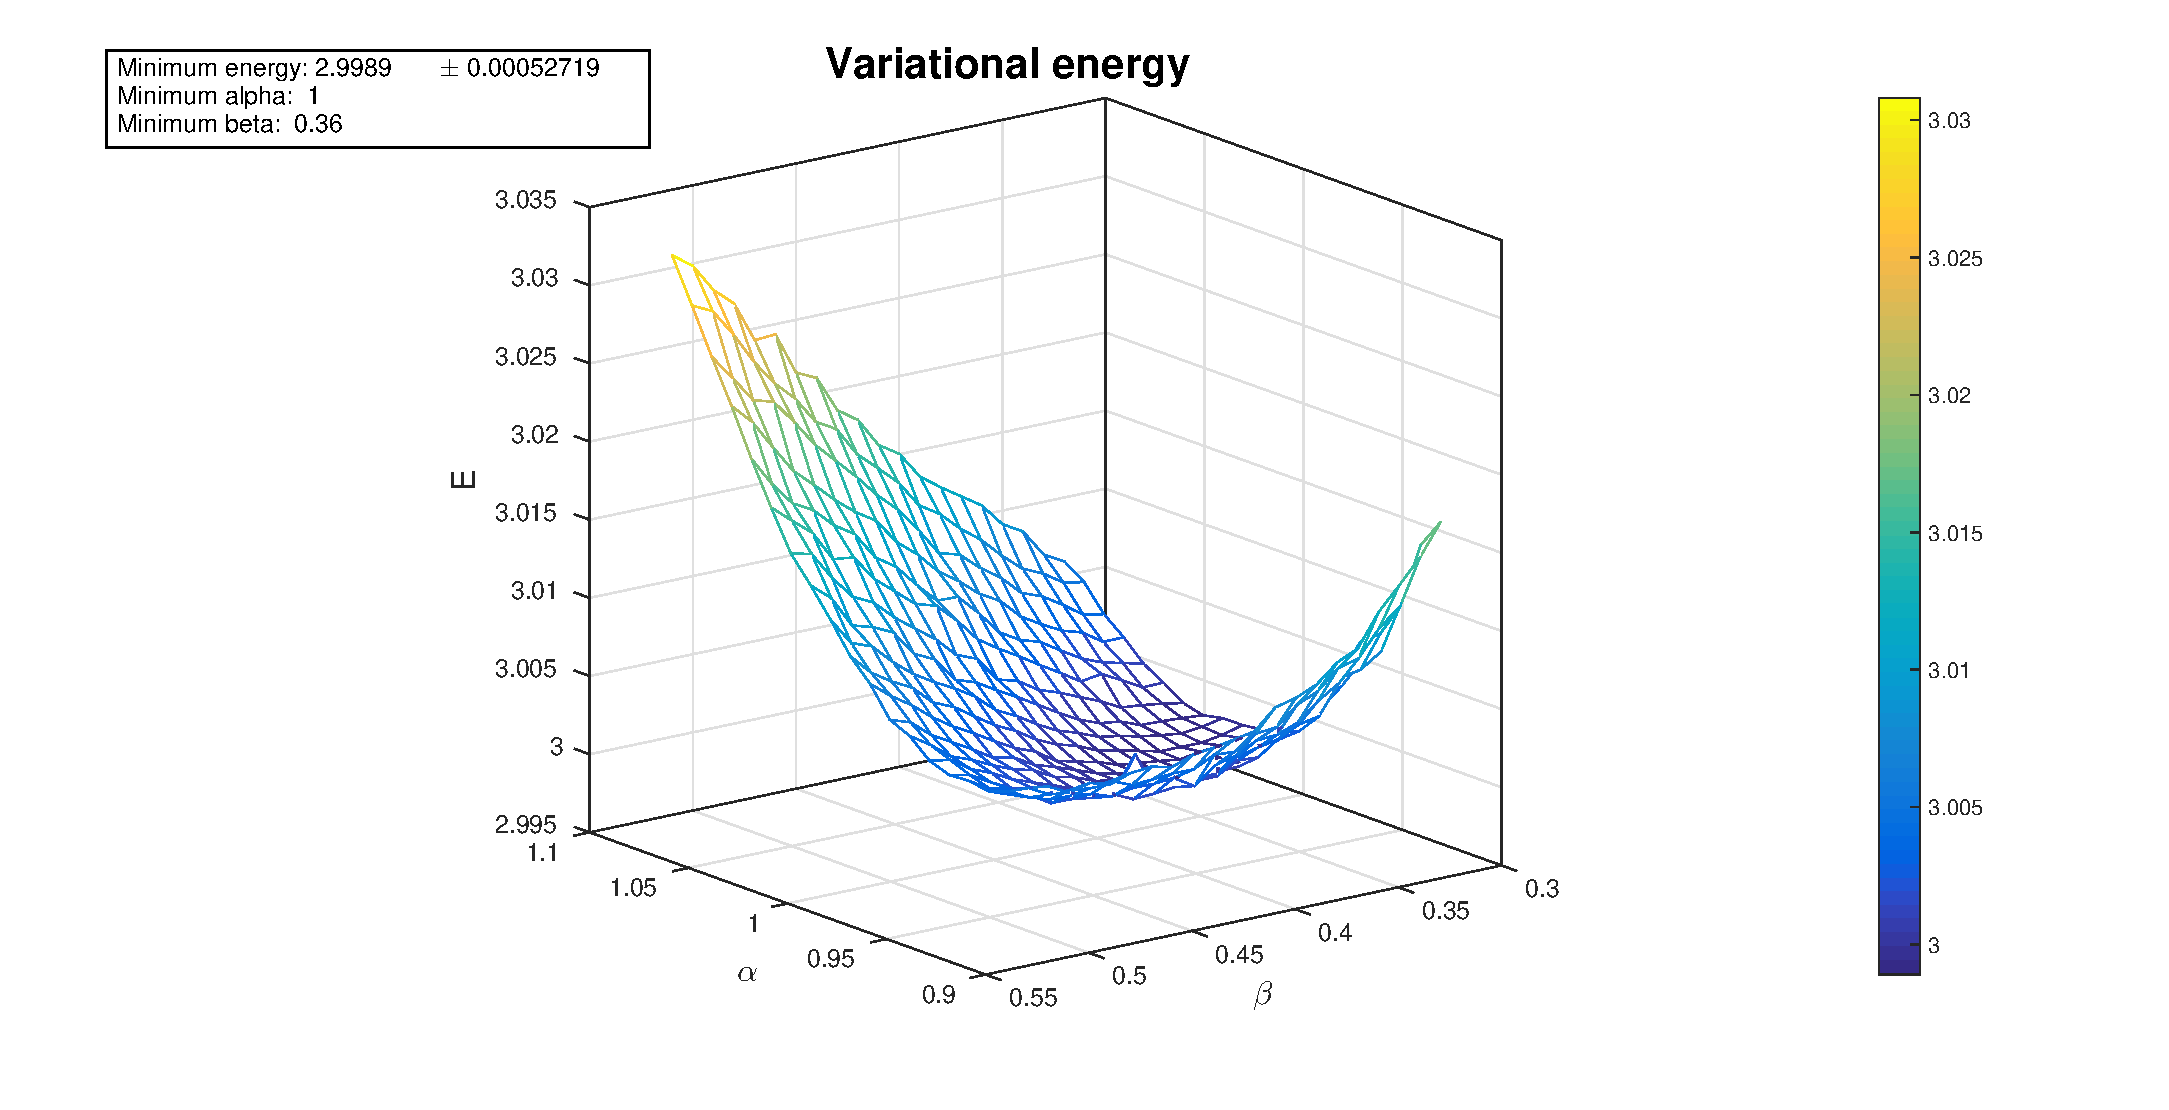
\includegraphics[width=\textwidth]{2e-rep_imp_high}
	\caption{The variational energy versus the variational parameters $\alpha$ and $\beta$. The settings used are: importance sampling with $\Delta t = 0.1$, Jastrow factor, parallelization (8 threads), $20$ variations of $\alpha$ and $\beta$ with step $0.01$, $\SI{2e5}{}$ Monte Carlo steps. Acceptance ratio is about $\SI{99.793}{\percent}$.}
	\label{fig:2e-rep_imp_high}
\end{figure}
%%%%%%%%%%%%%%%%%%%%%%%%%%%%%%%%%%%%%%%%%%%%%%%%%%%%%%%%%%%
%                                                         %
% CHAPTER 04:                                             %
% The 6-electrons system                                  %
%                                                         %
% This file is part of a BSc Thesis Project. See the      %
% LICENSE file for more information about licensing.      %
%                                                         %
% Author:     Matteo Seclì <secli.matteo@gmail.com>       %
% A.Y.:       2014/2015                                   %
% URL:        https://github.com/matteosecli/QMC          %
%                                                         %
%%%%%%%%%%%%%%%%%%%%%%%%%%%%%%%%%%%%%%%%%%%%%%%%%%%%%%%%%%%

\graphicspath{{Mainmatter/figures/PNG/}{Mainmatter/figures/PDF/}{Mainmatter/figures/}}

\chapter{The 6-electrons system}

\begin{figure}[H]
	\centering
	\definecolor{myblue}{rgb}{0,0.447,0.741}	
	\begin{tikzpicture}
		\tikzset{>=latex}
		
		%0,0
		\draw [ultra thick] (-1,0) -- (1,0) node[midway,below,align=center] {\scriptsize $n_x=0$ \\ \scriptsize $n_y=0$};
		\draw [very thick, myblue, ->] (-0.5,-0.5) -- (-0.5,0.5);
		\draw [very thick, myblue, ->] (0.5,0.5) -- (0.5,-0.5);
		
		%1,0
		\draw [ultra thick] (-2.5,2) -- (-0.5,2) node[midway,below,align=center] {\scriptsize $n_x=1$ \\ \scriptsize $n_y=0$};
		\draw [very thick, myblue, ->] (-2,1.5) -- (-2,2.5);
		\draw [very thick, myblue, ->] (-1,2.5) -- (-1,1.5);
		
		%0,1
		\draw [ultra thick] (0.5,2) -- (2.5,2) node[midway,below,align=center] {\scriptsize $n_x=0$ \\ \scriptsize $n_y=1$};
		\draw [very thick, myblue, ->] (1,1.5) -- (1,2.5);
		\draw [very thick, myblue, ->] (2,2.5) -- (2,1.5);
	\end{tikzpicture}
	\caption{The 6-electrons system configuration.}
	\label{eq:sketch_6e}
\end{figure}

The formulae discussed in the previous sections can be generalized for a $N$ electrons case. The trial wave function can be written as
\begin{equation}
	\psi_T(\vec{r}_1 \dots \vec{r}_N)= A \,  \text{Det}(S) \prod_{i<j}^N e^{\frac{r_{ij}}{1+\beta r_{ij}}},
\end{equation}
where $\text{Det}(S)$ is the Slater determinant
\begin{equation}
	\text{Det}(S)= \left|
	\begin{matrix}
		\phi_1(\vec{r}_1) & \phi_2(\vec{r}_1) & \dots & \phi_N(\vec{r}_1) \\
		\phi_1(\vec{r}_2) & \phi_2(\vec{r}_2) & \dots & \phi_N(\vec{r}_1) \\
		\vdots &  &  & \vdots \\
		\phi_1(\vec{r}_N) & \phi_2(\vec{r}_N) & \dots & \phi_N(\vec{r}_N) \\
	\end{matrix}
	\right|
\end{equation}

As we did in Section \ref{sec:considerations}, this determinant can be further simplified if we label our electrons in a smart way, as shown in \cite{Hjorth-Jensen2014}.

Let's consider a spin-independent quantum mechanical operator $\hat{O}(\vec{r}) $ acting on our trial wave function. The latter depends on $\vec{x} = (\vec{r}, \sigma) $ where $\vec{r}$ includes the space coordinates and $\sigma$ the spin coordinates.
We have that:
\begin{equation}
	\Braket{\hat{O}} = \frac{\Braket{\psi_T(\vec{x})|\hat{O}(\vec{r})|\psi_T(\vec{x})}}{\Braket{\psi_T(\vec{x})|\psi_T(\vec{x})}}
\end{equation}

Now we can replace the total antisymmetric wave function with one with permuted arguments and we can arbitrarily choose that the first $N/2$ arguments are spin up and the other half are spin down. We get:
\begin{align}
	\psi_T(\vec{x_1},\ldots,\vec{x_N}) 
	\longrightarrow& \, \psi_t(\vec{x_{i1}},\ldots,\vec{x_{iN}}) \\
	=& \, \psi_T(\{\vec{r_{i1}}, \uparrow\},\ldots,\{\vec{r_{iN/2}}, \uparrow\},\{\vec{r_{i1}}, \downarrow\},\ldots,\{\vec{r_{iN/2}}, \downarrow\}) \\
	=& \, \psi_T(\{\vec{r_{1}}, \uparrow\},\ldots,\{\vec{r_{N/2}}, \uparrow\},\{\vec{r_{N/2 +1}}, \downarrow\},\ldots,\{\vec{r_{N}}, \downarrow\})
\end{align}
The operator $\hat{O}$ is symmetric with the respect to the exchange of labels in a pair of particles, so:
\begin{equation}
	\Braket{\hat{O}} = \frac{\Braket{\psi_T(\vec{r})|\hat{O}(\vec{r})|\psi_T(\vec{r})}}{\Braket{\psi_T(\vec{r})|\psi_T(\vec{r})}}
\end{equation}

The wave function is now antisymmetric with respect to exchange of spatial coordinates of pairs of spin-up or spin-down electrons. Therefore, for spin-independent Hamiltonians, the Slater determinant can be splitted in a product of two Slater determinants, one for the single particle orbitals with spin up and the other with single particle orbitals with spin down. We have then:
\begin{equation}
	\psi_S = S^{\uparrow}S^{\downarrow}
\end{equation}
where
\begin{equation}
	S^{\uparrow} = \left|
	\begin{matrix}
		\phi_1(\vec{r}_1) & \phi_2(\vec{r}_1) & \dots & \phi_{N/2}(\vec{r}_1) \\
		\phi_1(\vec{r}_2) & \phi_2(\vec{r}_2) & \dots & \phi_{N/2}(\vec{r}_1) \\
		\vdots &  &  & \vdots \\
		\phi_1(\vec{r}_{N/2}) & \phi_2(\vec{r}_{N/2}) & \dots & \phi_{N/2}(\vec{r}_{N/2}) \\
	\end{matrix}
	\right|
\end{equation}
and  $S^{\downarrow}$ is obviously defined in a similar way. The $\phi_i$'s functions are just as the one defined in equation (\ref{eq:phi_qnums}).

So, our final trial wave-function is just
\begin{equation}
	\psi_T = |S^{\uparrow}||S^{\downarrow}|J
\end{equation}
being $J$ the Padé-Jastrow factor.

The C++ implementation of $\psi_S$ is therefore straightforward and it is shown below.

\begin{lstlisting}[language=cpp]
	double Orbitals::SlaterD(mat& r) {
	    mat D_up(n_half,n_half), D_down(n_half,n_half);
	
	    for (int i = 0; i < n_half; i++) {
	        this->set_qnum_indie_terms(r, i);
	        for (int j = 0; j < n_half; j++) {
	            D_up(i,j) = this->phi(r, i, j);
	        }
	    }
	
	    for (int i = 0; i < n_half; i++) {
	        this->set_qnum_indie_terms(r, i+n_half);
	        for (int j = 0; j < n_half; j++) {
	            D_down(i,j) = this->phi(r, i+n_half, j);
	        }
	    }
	
	    double slater = det(D_up)*det(D_down);
	
	    D_up.reset();
	    D_down.reset();
	
	    return slater;
	}
\end{lstlisting}


\section{$\omega = 0.28$}

We start by studying our system for $\omega = 0.28$. A preliminary and very rough result is shown in Figure \ref{fig:6e-028-rep}.
\begin{figure}[H]
	\centering
	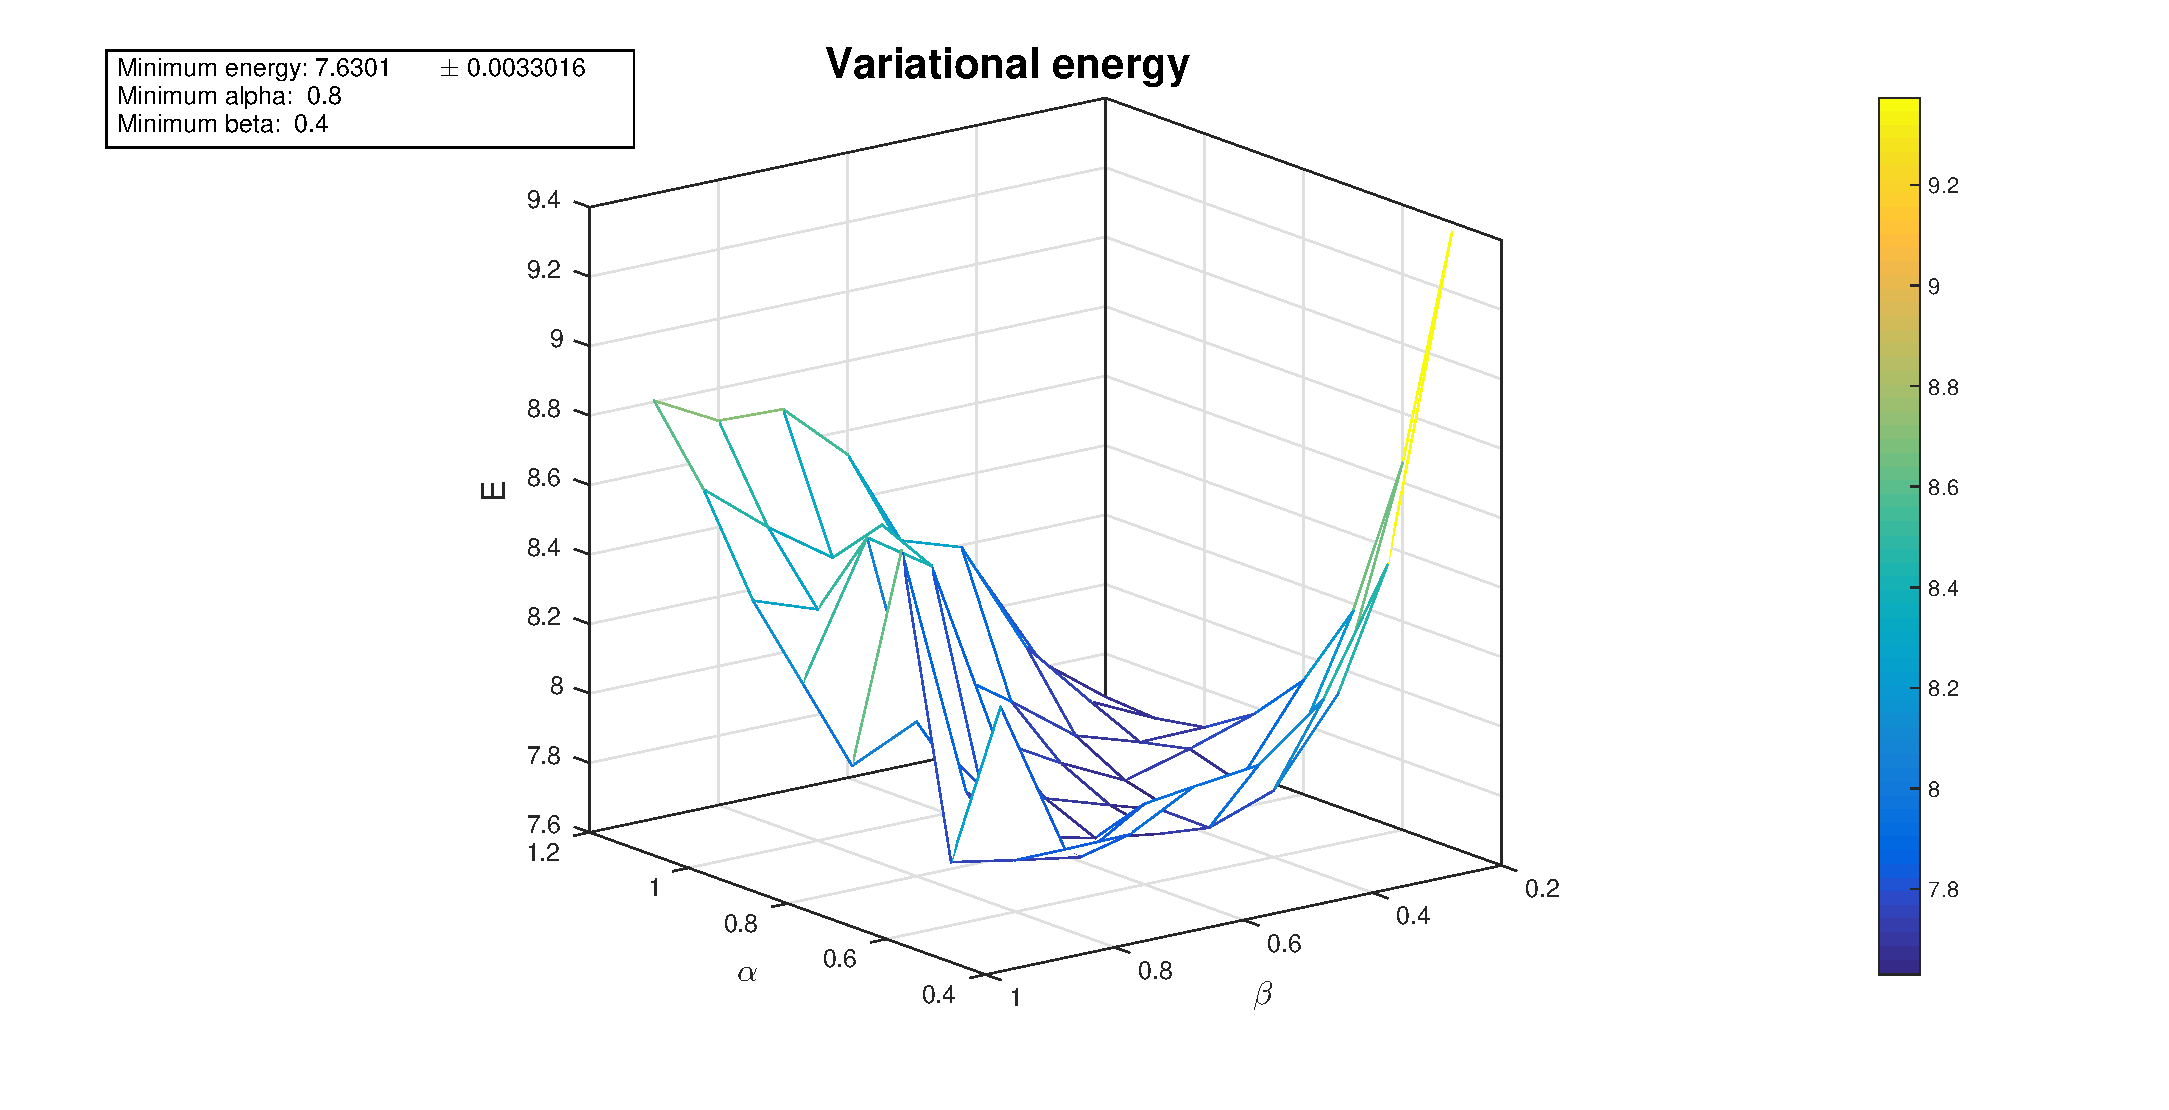
\includegraphics[width=\textwidth]{6e-028-rep}
	\caption{The variational energy versus the variational parameters $\alpha$ and $\beta$. The settings used are: importance sampling with $\Delta t = 0.1$, Jastrow factor, parallelization (8 threads), $8$ variations of $\alpha$ and $\beta$ with step $0.1$, $\SI{1e5}{}$ Monte Carlo steps. $\omega=0.28$.}
	\label{fig:6e-028-rep}
\end{figure}
Restricting to the significant region, we get the result in Figure \ref{fig:6e-028-rep_fine}.
\begin{figure}%[H]
	\centering
	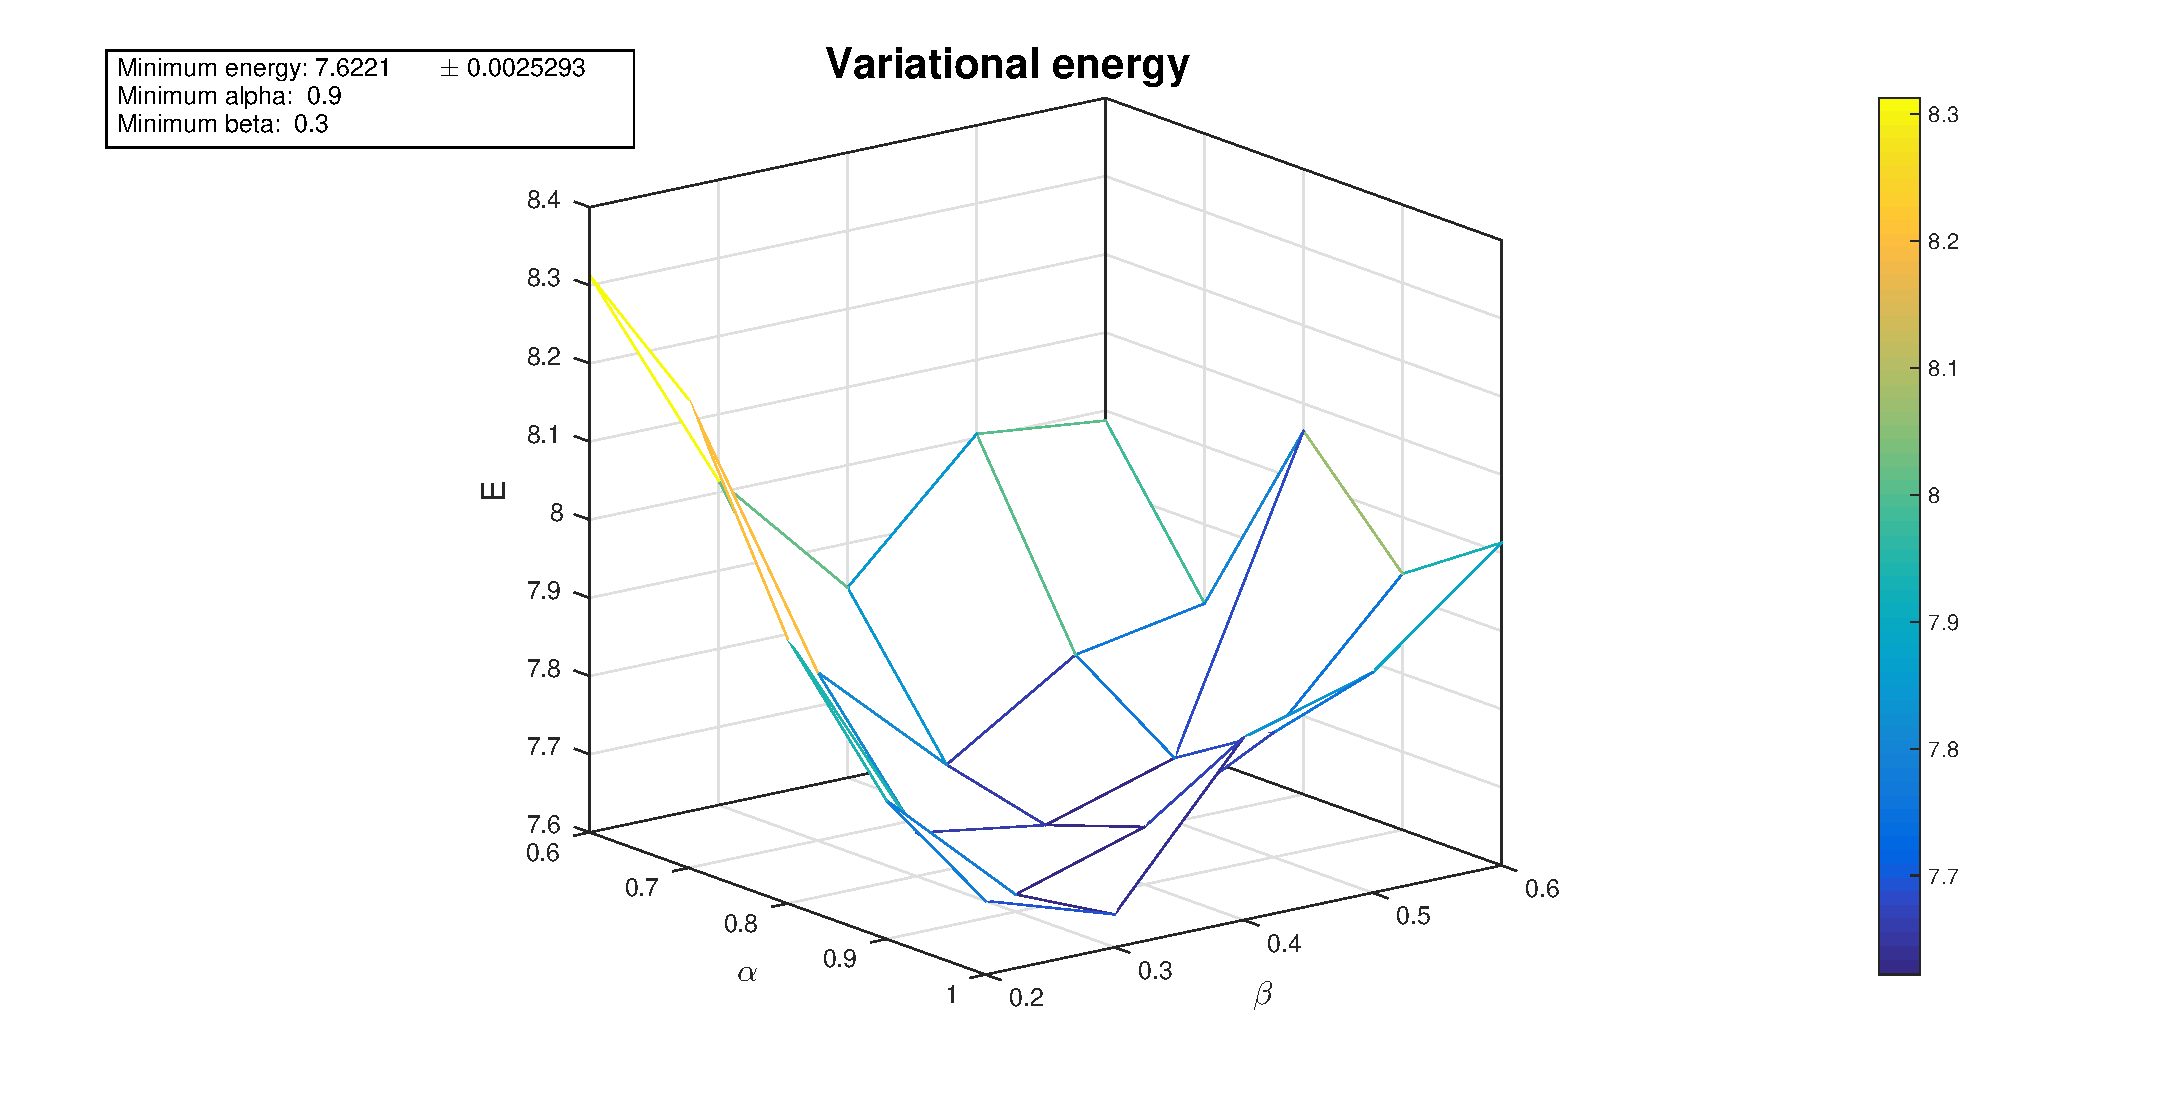
\includegraphics[width=\textwidth]{6e-028-rep_fine}
	\caption{The variational energy versus the variational parameters $\alpha$ and $\beta$. The settings used are: importance sampling with $\Delta t = 0.1$, Jastrow factor, parallelization (8 threads), $5$ variations of $\alpha$ and $\beta$ with step $0.1$, $\SI{2e5}{}$ Monte Carlo steps. $\omega=0.28$.}
	\label{fig:6e-028-rep_fine}
\end{figure}

You see that the plot is no more nice like the 2-electrons case, mainly because we didn't used enough Monte Carlo steps. The problem is that now the program has to calculate $3 \times 3$ determinants every time, so it's much slower than the previous case. To refine the result, we just doubled the number of Monte Carlo loops and restricted a little bit the variational parameters grid; taking a finer grid with more Monte Carlo cycles would have required ages, literally.

Anyway, still with this configuration, we get a result that is really near the one calculated by DMC in \cite{PedersenLohne2011}, that turns out to be $\SI{7.6001 \pm 0.0001}{\atomicunit}$.

A nice way to test the Slater determinant code is to turn off the electron-electron repulsion. In that case, $\psi_S$ is the \emph{exact} solution (for $\alpha = 1$). We already showed in Section \ref{sec:2e_unp} that the ground-state energy for the single electron is $E_s = \hbar\omega(n_x + n_y + 1)$. Since -- in the 6 electrons case -- we have 2 electrons with $n_x + n_y = 0$ and 4 electrons with $n_x + n_y = 1$ (See Figure \ref{eq:sketch_6e}), the total energy for the ground state is
\begin{equation}
	E_{\text{gs}} = \hbar\omega\left[2(0+1)+4(1+1)\right] = 10\omega.
\end{equation}

Turning off the repulsion results in a minimum $E_{\text{gs}} = \SI{2.7999999999999 \pm 0.0000000000002}{\atomicunit}$ for $\alpha=1$, that confirms the prediction.

\section{$\omega = 0.5$}
We repeat the same calculations with $\omega=0.5$, obtaining the results in Figure \ref{fig:6e-050-rep}.
\begin{figure}[H]
	\centering
	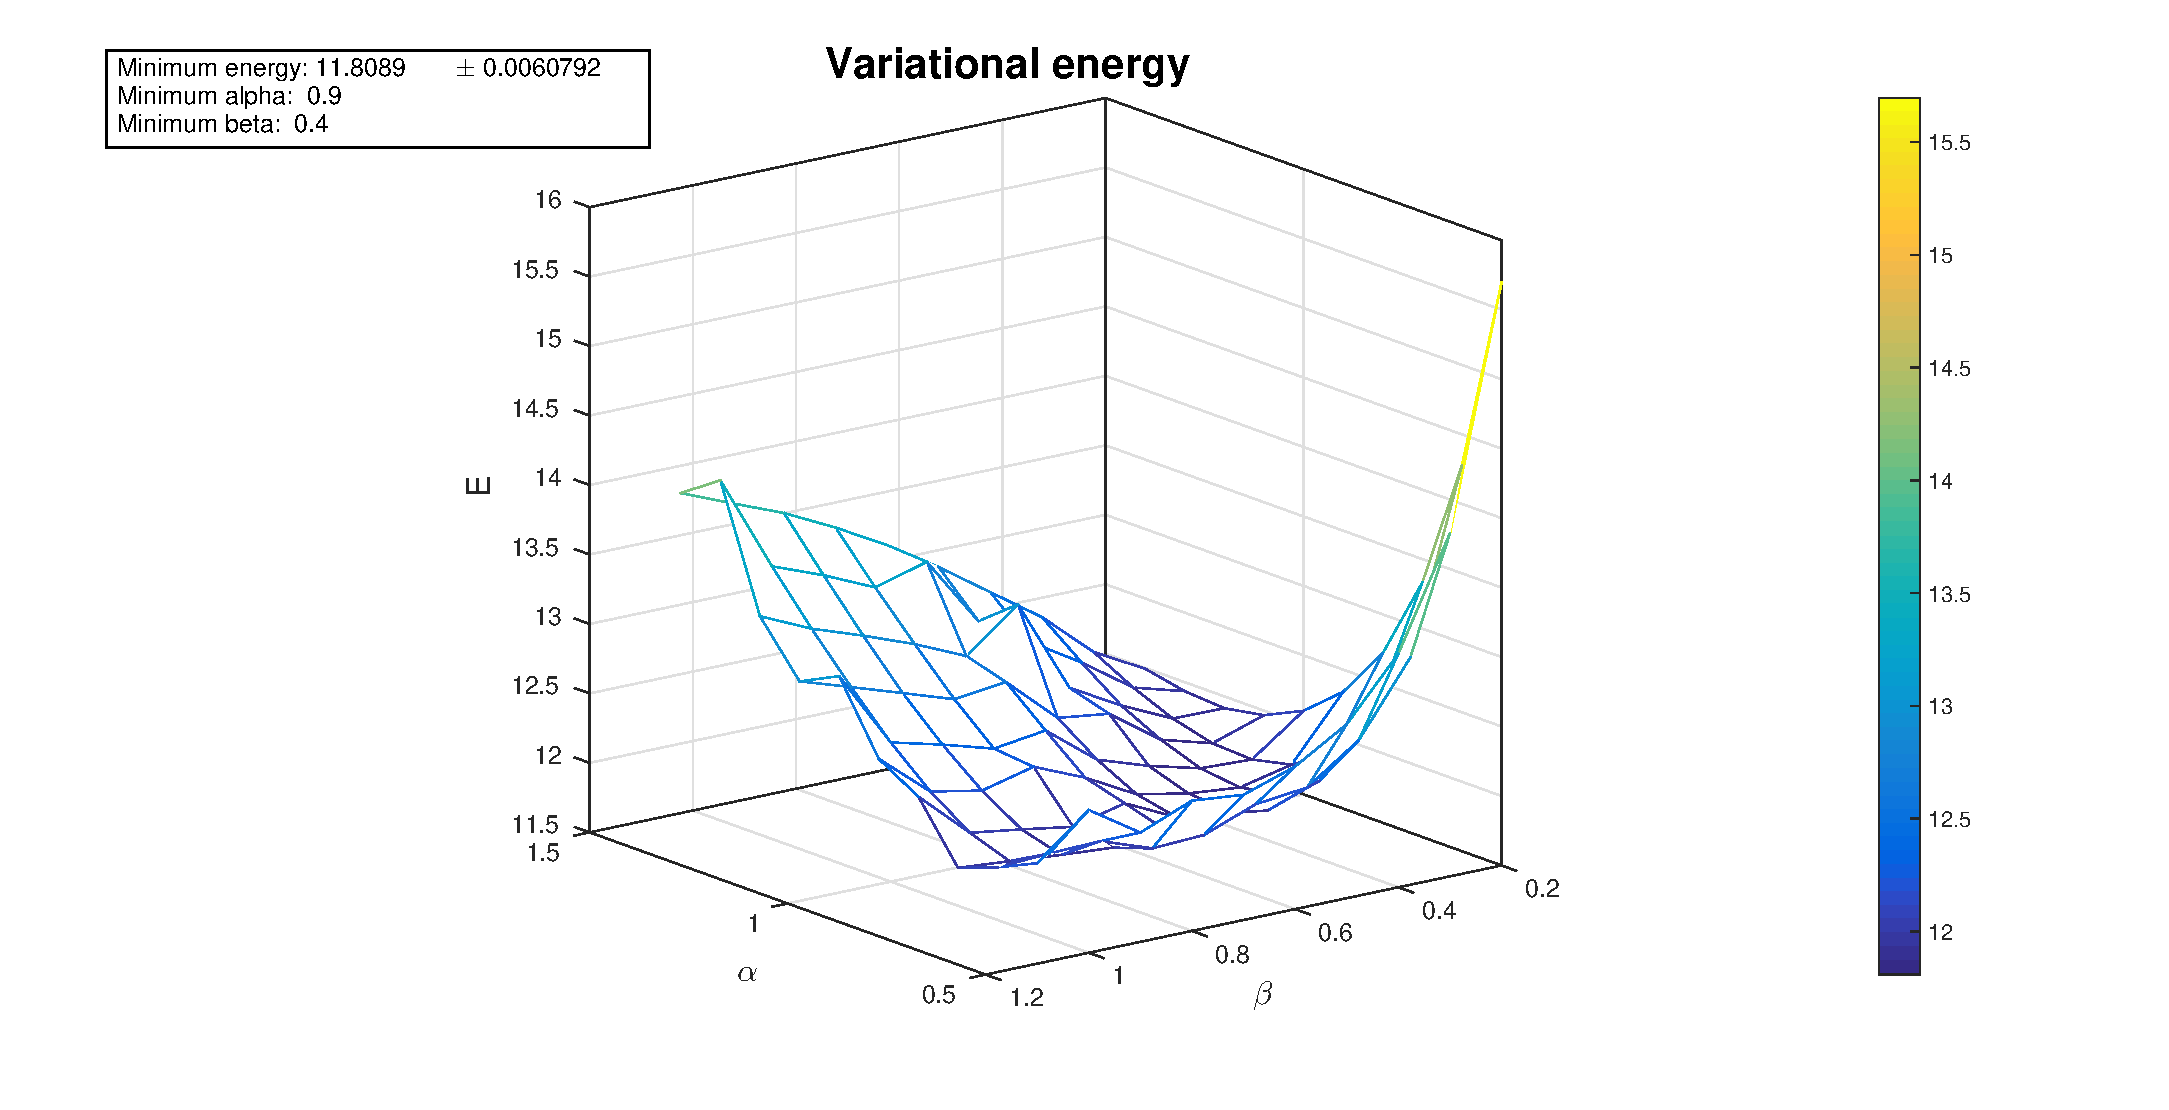
\includegraphics[width=\textwidth]{6e-050-rep}
	\caption{The variational energy versus the variational parameters $\alpha$ and $\beta$. The settings used are: importance sampling with $\Delta t = 0.1$, Jastrow factor, parallelization (8 threads), $10$ variations of $\alpha$ and $\beta$ with step $0.1$, $\SI{2e5}{}$ Monte Carlo steps. $\omega=0.50$.}
	\label{fig:6e-050-rep}
\end{figure}

Again, our result is pretty consistent with the one calculated by DMC in \cite{PedersenLohne2011}, that is $\SI{11.7888 \pm 0.0002}{\atomicunit}$.

\section{$\omega = 1$}

Just with the same parameters used in Figure \ref{fig:6e-050-rep} but changing the frequency to $\omega=1.00$, we have the results in Figure \ref{fig:6e-100-rep}.
\begin{figure}[H]
	\centering
	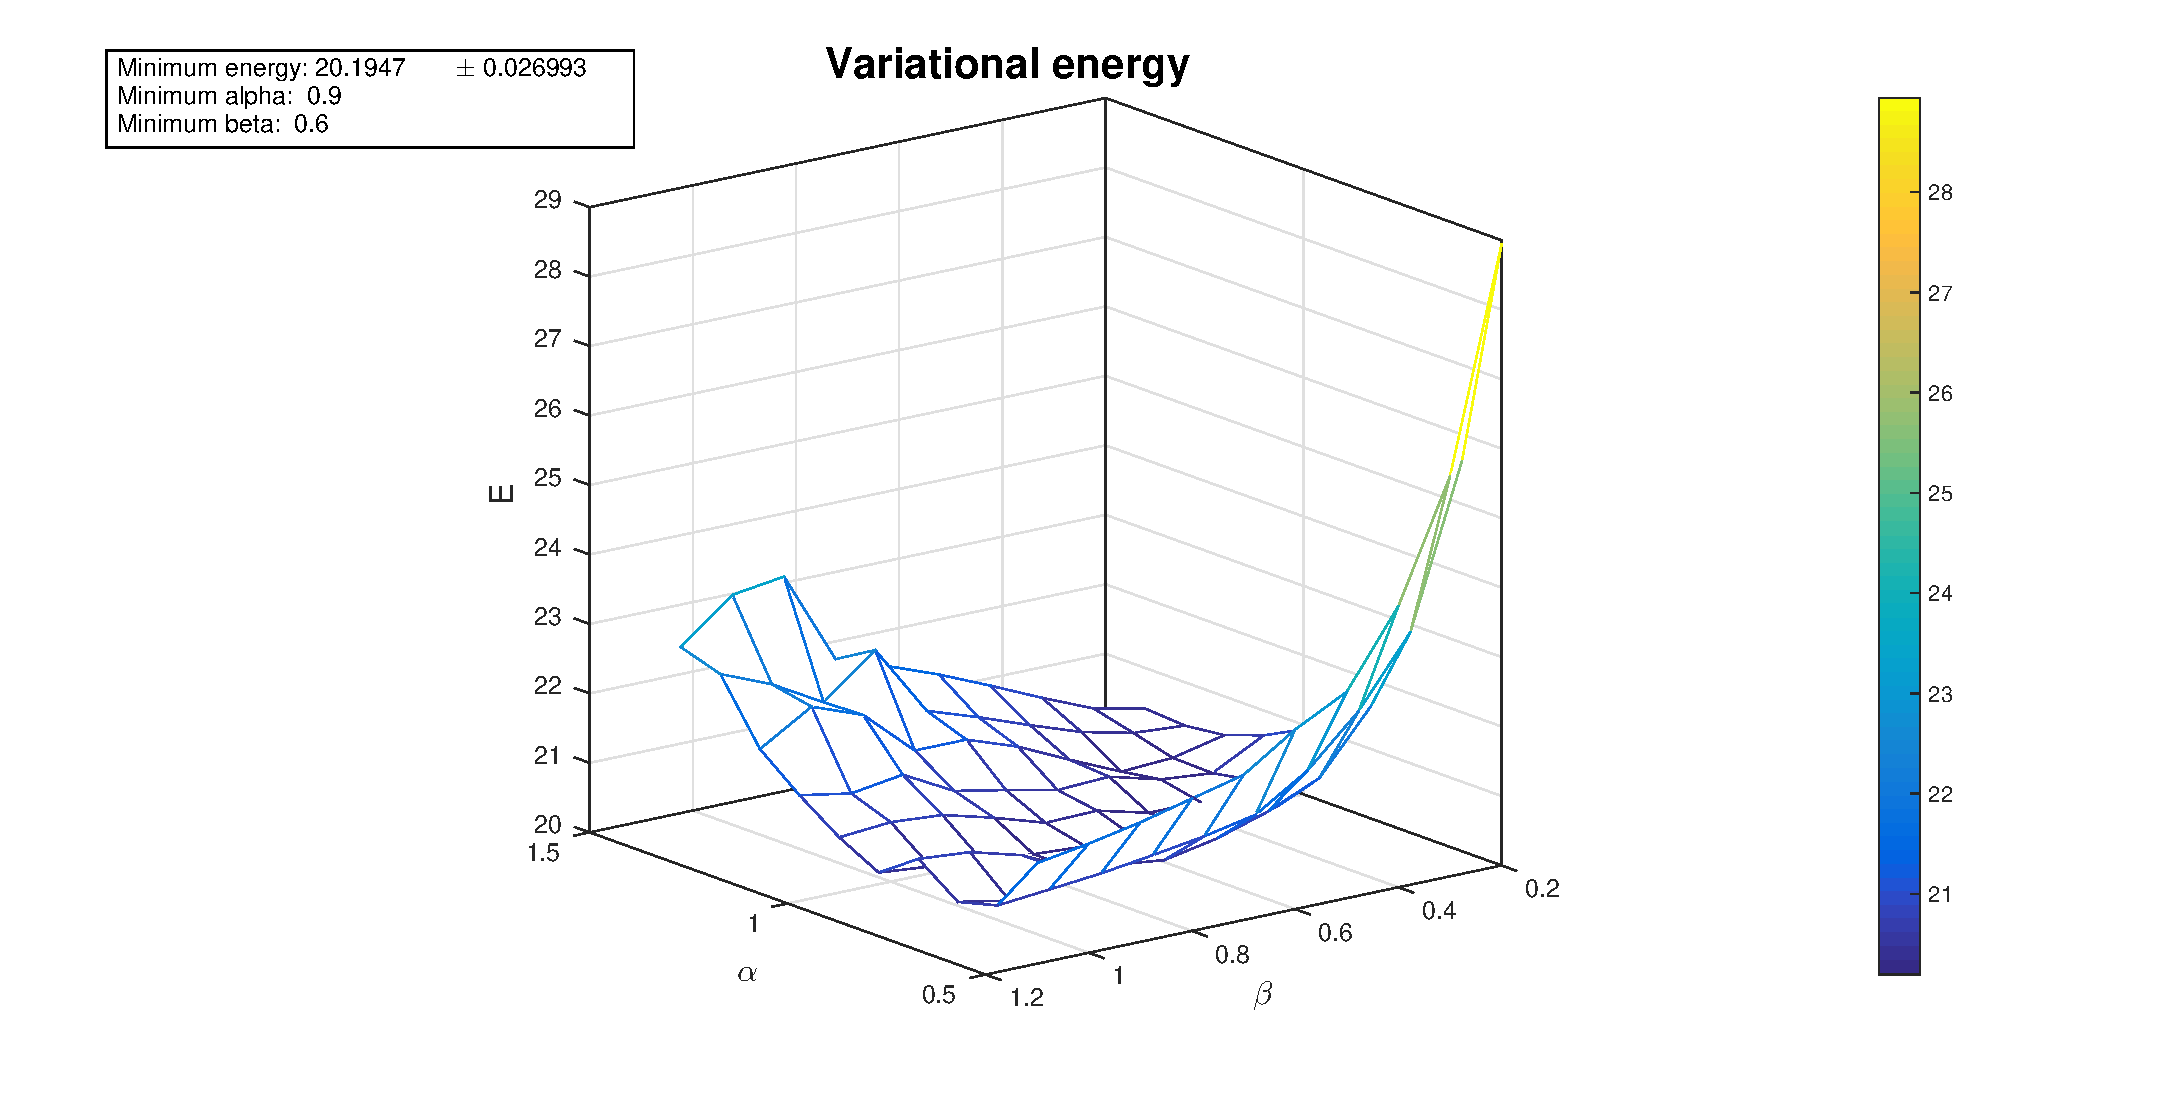
\includegraphics[width=\textwidth]{6e-100-rep}
	\caption{The variational energy versus the variational parameters $\alpha$ and $\beta$. The settings used are: importance sampling with $\Delta t = 0.1$, Jastrow factor, parallelization (8 threads), $10$ variations of $\alpha$ and $\beta$ with step $0.1$, $\SI{2e5}{}$ Monte Carlo steps. $\omega=1.00$.}
	\label{fig:6e-100-rep}
\end{figure}

Once again, our result is in very good accordance with the one calculated by DMC in \cite{PedersenLohne2011}, that is $\SI{20.1597 \pm 0.0002}{\atomicunit}$.
%%%%%%%%%%%%%%%%%%%%%%%%%%%%%%%%%%%%%%%%%%%%%%%%%%%%%%%%%%%
%                                                         %
% CHAPTER 05:                                             %
% The virial theorem                                      %
%                                                         %
% This file is part of a BSc Thesis Project. See the      %
% LICENSE file for more information about licensing.      %
%                                                         %
% Author:     Matteo Seclì <secli.matteo@gmail.com>       %
% A.Y.:       2014/2015                                   %
% URL:        https://github.com/matteosecli/QMC          %
%                                                         %
%%%%%%%%%%%%%%%%%%%%%%%%%%%%%%%%%%%%%%%%%%%%%%%%%%%%%%%%%%%

\graphicspath{{Mainmatter/figures/PNG/}{Mainmatter/figures/PDF/}{Mainmatter/figures/}}

\chapter{The virial theorem}
\label{chap:virial}

The virial theorem states that, if the potential energy has the form $V(r) \sim r^n$ -- where $r$ is the interparticle distance, then $\Braket{T} = \frac{2}{n}\Braket{V}$. For a pure harmonic oscillator, this theorem is simply the \emph{equipartition theorem}:
\begin{equation}
	\Braket{T} = \Braket{V}.
\end{equation}
This is quite easy to prove. Let's introduce the ladder operators
\begin{equation}
	\hat{a}=\frac{1}{\sqrt{2 \hbar \omega m}} \left( m \omega \hat{x}+ i \hat{p} \right)
	\qquad \text{and} \qquad
	\hat{a}^{\dagger}=\frac{1}{\sqrt{2 \hbar \omega m}} \left( m \omega \hat{x}- i \hat{p} \right)
\end{equation}
It can be shown that these operators act on the harmonic oscillator eigenstates such that
\begin{equation}
	\hat{a} \Ket{n} =\sqrt{n} \Ket{n-1}
	\quad \text{and} \quad 
	\hat{a}^{\dagger} \Ket{n} =\sqrt{n+1} \Ket{n+1},
\end{equation}
and we also have
\begin{equation}
	N\Ket{n} \doteqdot \hat{a}^{\dagger}\hat{a}\Ket{n} = n\Ket{n}.
\end{equation}

Using these properties, the calculation of the expected value of the potential energy is straightforward:
\begin{align}
	\Braket{n|\frac{1}{2}m\omega^2\hat{x}^2|n}
	&= \frac{1}{2}m\omega^2\Braket{n|\hat{x}^2|n} \\
	&= \frac{1}{2}\cancel{m}\omega^{\cancel{2}}\frac{\hbar}{2\cancel{m}\cancel{\omega}}\Braket{n|\left(\hat{a}^{\dagger}+\hat{a}\right)\left(\hat{a}+\hat{a}^{\dagger}\right)|n} \\
	&= \frac{\hbar\omega}{4} \left(\Braket{n|\hat{a}^{\dagger}\hat{a}^{\dagger}|n}+\Braket{n|\hat{a}\hat{a}^{\dagger}|n}+\Braket{n|\hat{a}^{\dagger}\hat{a}|n}+\Braket{n|\hat{a}\hat{a}|n}\right) \\
	&= \frac{\hbar\omega}{4} \left(\sqrt{n+2}\sqrt{n+1}\cancelto{0}{\Braket{n|n+2}}\right. \nonumber \\
	&\left.+\Braket{n|\hat{N}+1|n}+\Braket{n|\hat{N}|n}+\sqrt{n}\sqrt{n-1}\cancelto{0}{\Braket{n|n-2}}\right) \\
	&= \frac{\hbar\omega}{4}((n+1)+n) = \frac{\hbar\omega}{4}(2n+1) \\
	&= \frac{\hbar\omega}{2}\left(n+\frac{1}{2}\right)
\end{align}
If we perform the same calculation for $\Braket{n|\frac{\hat{p}^2}{2m}|n}$ (the expected value of the kinetic energy) we will obtain the same result, yielding
\begin{equation}
	\Braket{T} = \Braket{V}
\end{equation}
and
\begin{equation}
	\Braket{T}+\Braket{V} = \hbar\omega\left(n+\frac{1}{2}\right),
\end{equation}
that is the total energy of the harmonic oscillator, as expected.

Let's now graph the ratio $\Braket{T} / \Braket{V}$ for different values of $\omega$.

\section{The 2-electrons system}

We firstly computed $\Braket{T}$ and $\Braket{V}$ \emph{without} the electron-electron repulsion, to check our code. We chose $\omega=0.01,\,0.28,\,0.50,\,0.70,\,1.00$. The result -- completely expected -- is shown in Figure \ref{fig:virial_2e-norep}.
\begin{figure}[h]%[H]
	\centering
	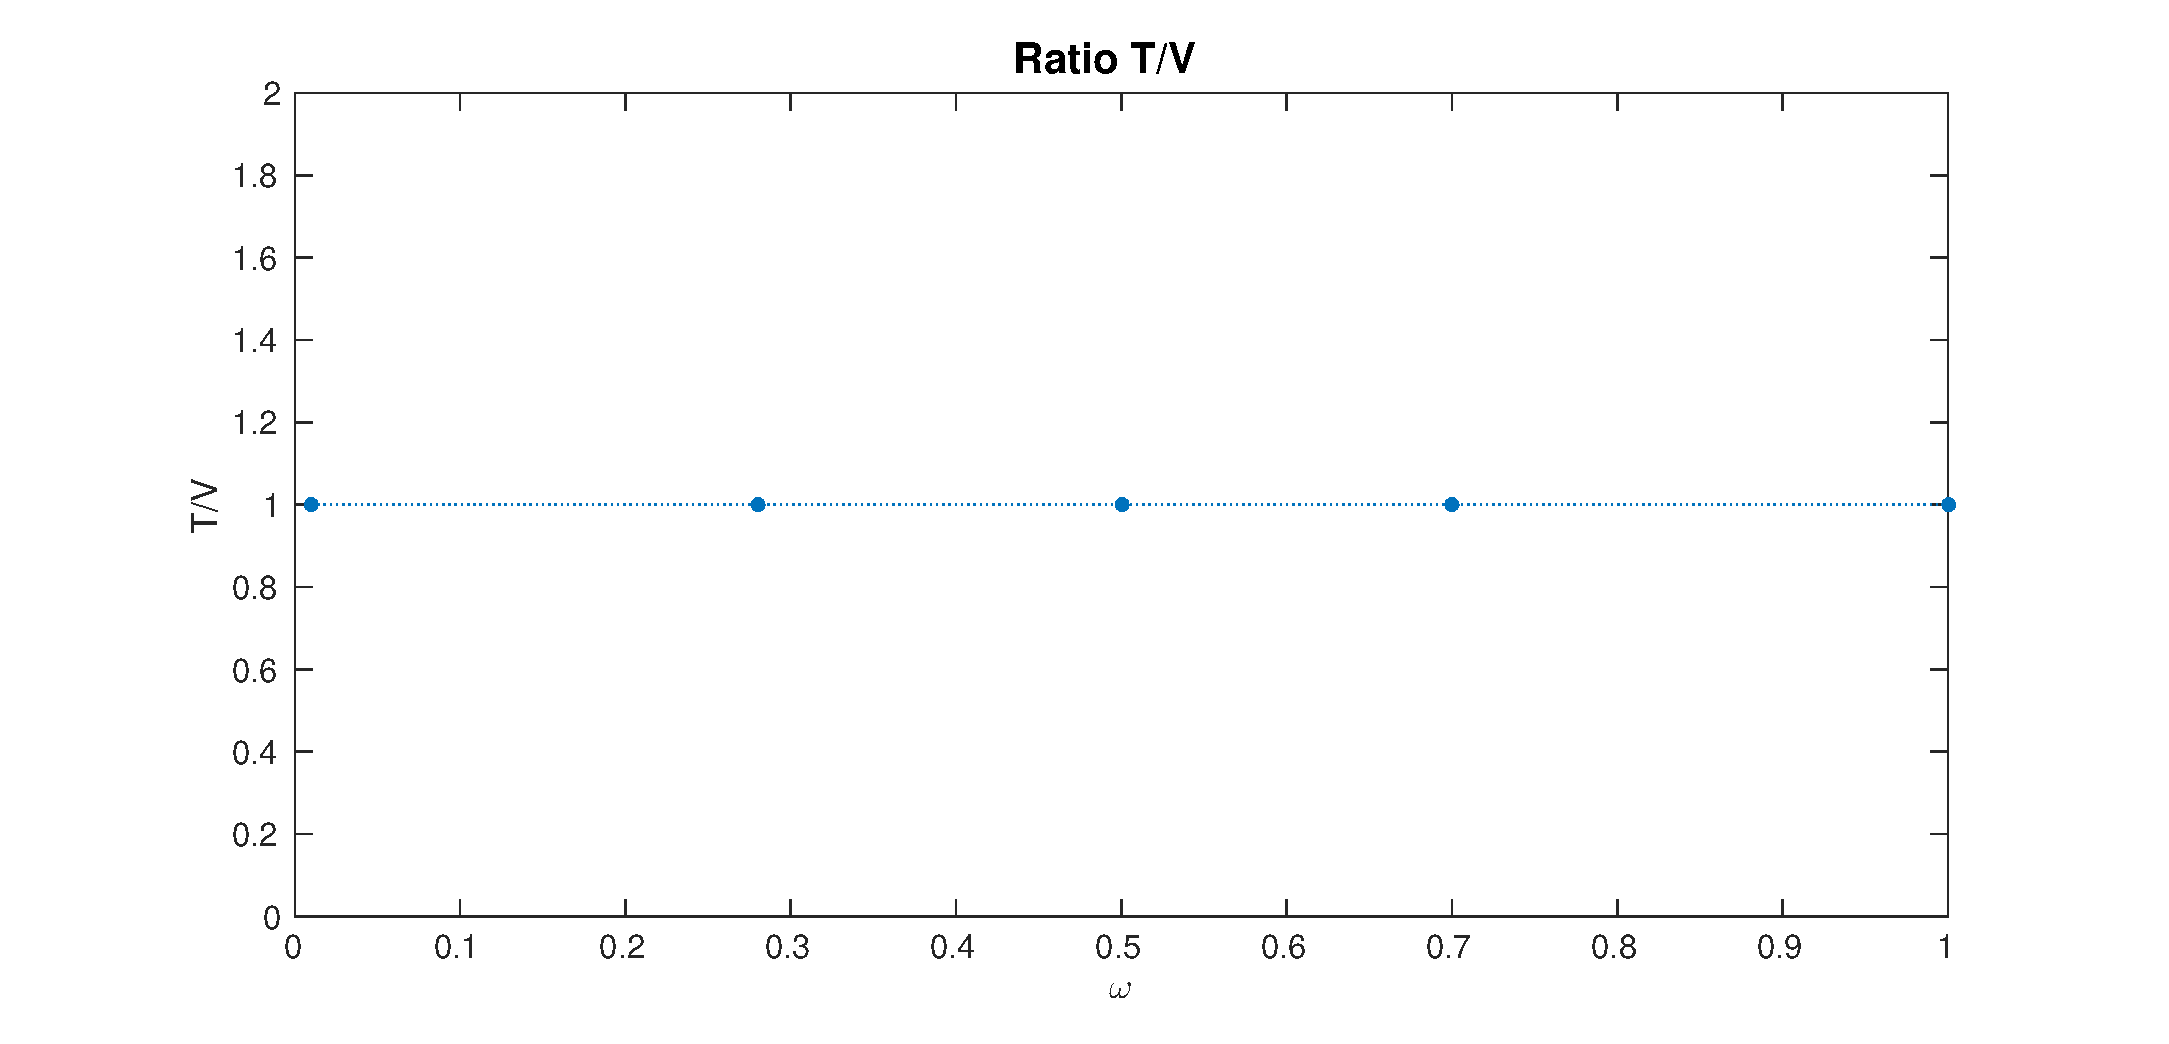
\includegraphics[width=\textwidth]{virial_2e-norep}
	\caption{The ratio $\Braket{T} / \Braket{V}$ for different values of $\omega$ and no electron-electron repulsion. The settings used are: importance sampling with $\Delta t = 0.1$, parallelization (8 threads), $\SI{1e7}{}$ Monte Carlo steps.}
	\label{fig:virial_2e-norep}
\end{figure}

After that, we added the electron-electron repulsion and we did again the calculations for the same $\omega$ values. The result, shown in Figure \ref{fig:virial_2e-rep}, is quite different.

The dashed line is a fit of the type
\begin{equation}
	\frac{\Braket{T}}{\Braket{V}} = b\log(c\omega),
\end{equation}
which gives $b = \SI{0.052 \pm 0.007}{}$ and $c = \SI{2340 \pm 2021}{}$. We can't really say if the behaviour of our data is logarithmic without a theoretical basis and with just $5$ points; the purpose of the dashed line in Figure \ref{fig:virial_2e-rep} is just to show that our data is \emph{no way} linear. This is due to the presence of the repulsive force, that can be dominant or not.

\begin{figure}[H]
	\centering
	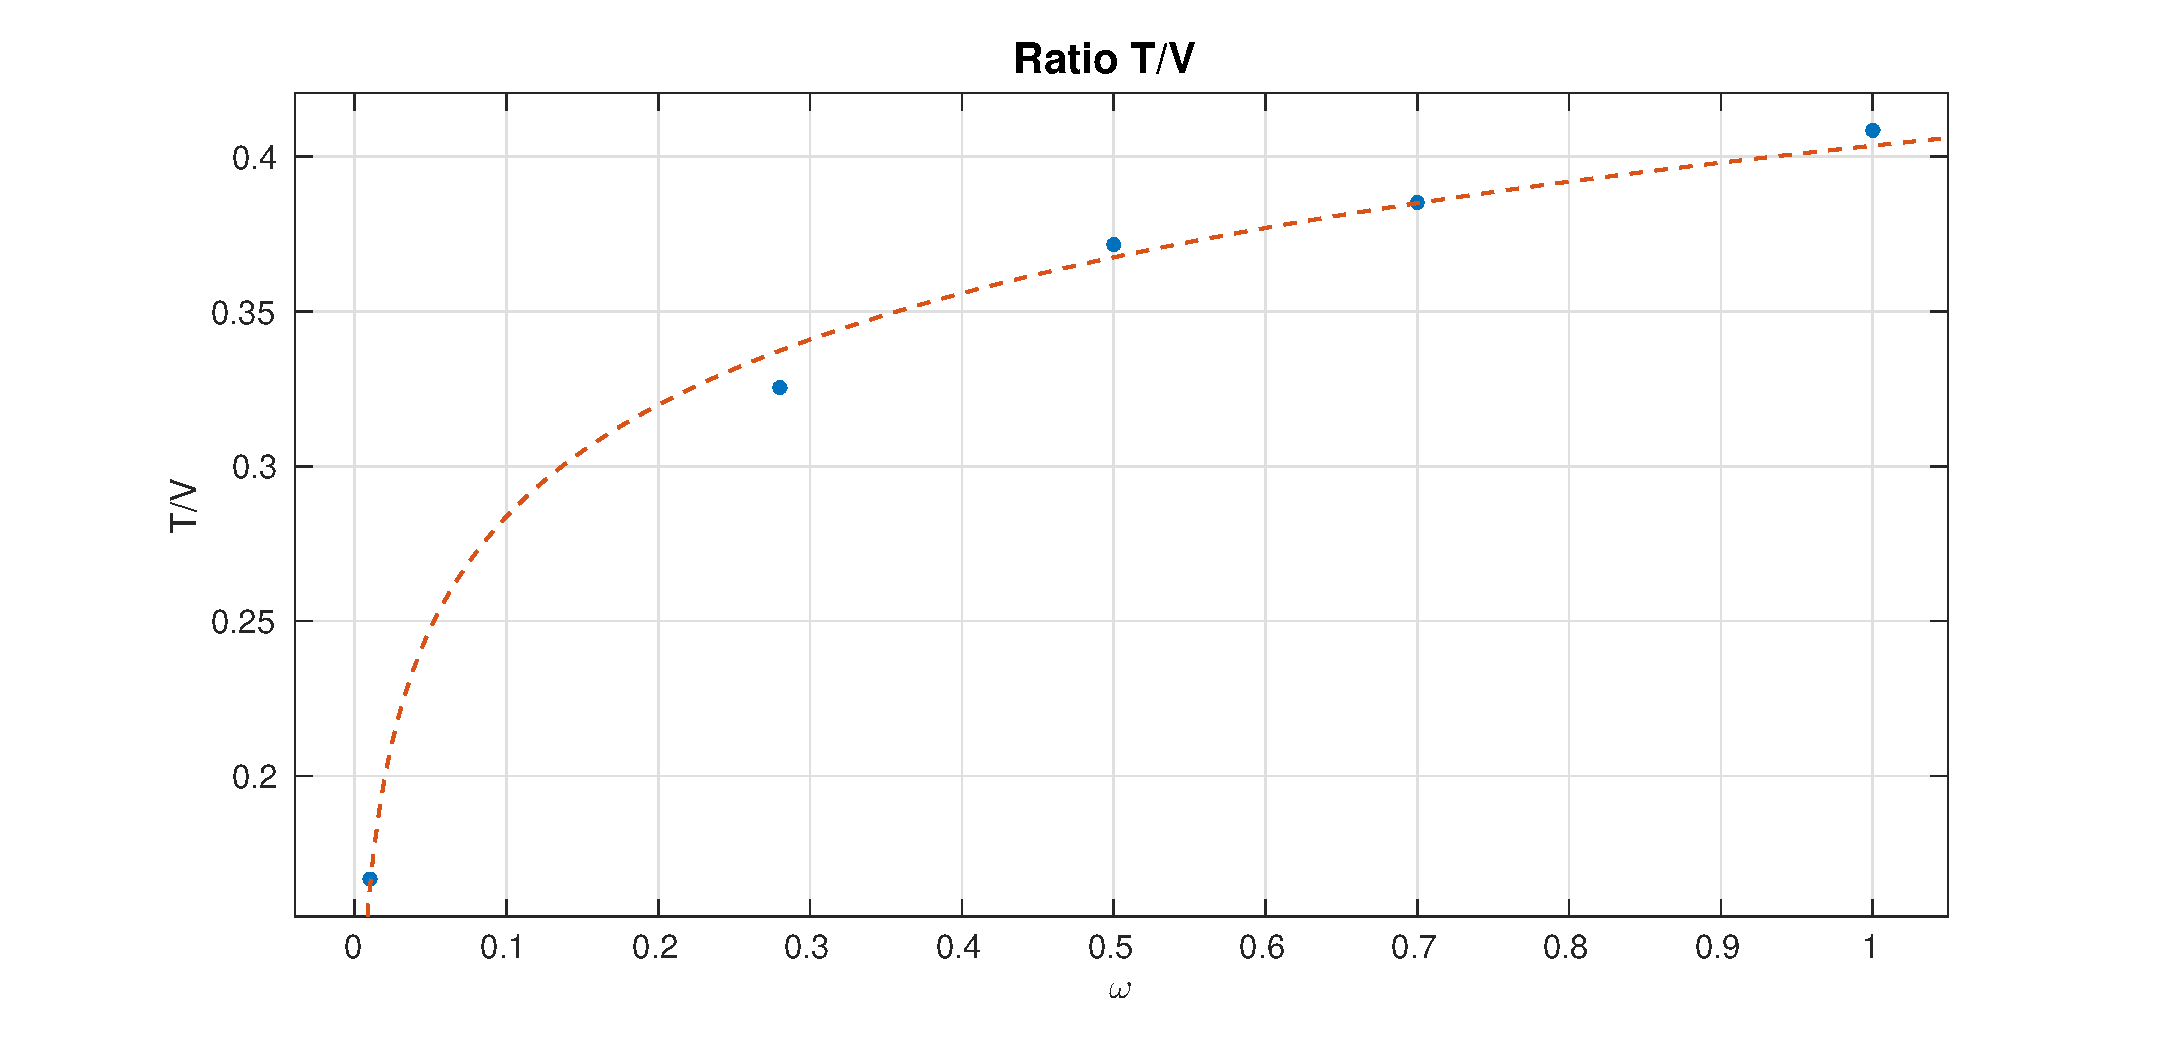
\includegraphics[width=\textwidth]{virial_2e-rep}
	\caption{The ratio $\Braket{T} / \Braket{V}$ for different values of $\omega$ with electron-electron repulsion. The settings used are: importance sampling with $\Delta t = 0.1$, Jastrow factor, parallelization (8 threads), $\SI{1e7}{}$ Monte Carlo steps. The fit is logarithmic.}
	\label{fig:virial_2e-rep}
\end{figure}

In a very intuitive way, we can at least say that what we obtain is coherent with the physics of the system. For $\omega \gg 1$ the oscillator potential is dominant and the repulsion can be considered as a small perturbation, which means that we have more kinetic energy than potential energy ($\Braket{T} > \Braket{V}$). For $\omega \ll 1$, we almost have only a repulsion potential plus a small harmonic perturbation; in other words, $\Braket{T} < \Braket{V}$.

If one really wants to find an analytical relation for the ratio $\Braket{T} / \Braket{V}$ of this system, he should compute the two terms separately in a way similar to the one shown at the beginning of Chapter \ref{chap:virial} and then take the ratio of them. Note that this is not always possible, since the necessary integrals could not be solved analytically.


\section{The 6-electrons system}

\begin{figure}[h]%[H]
	\centering
	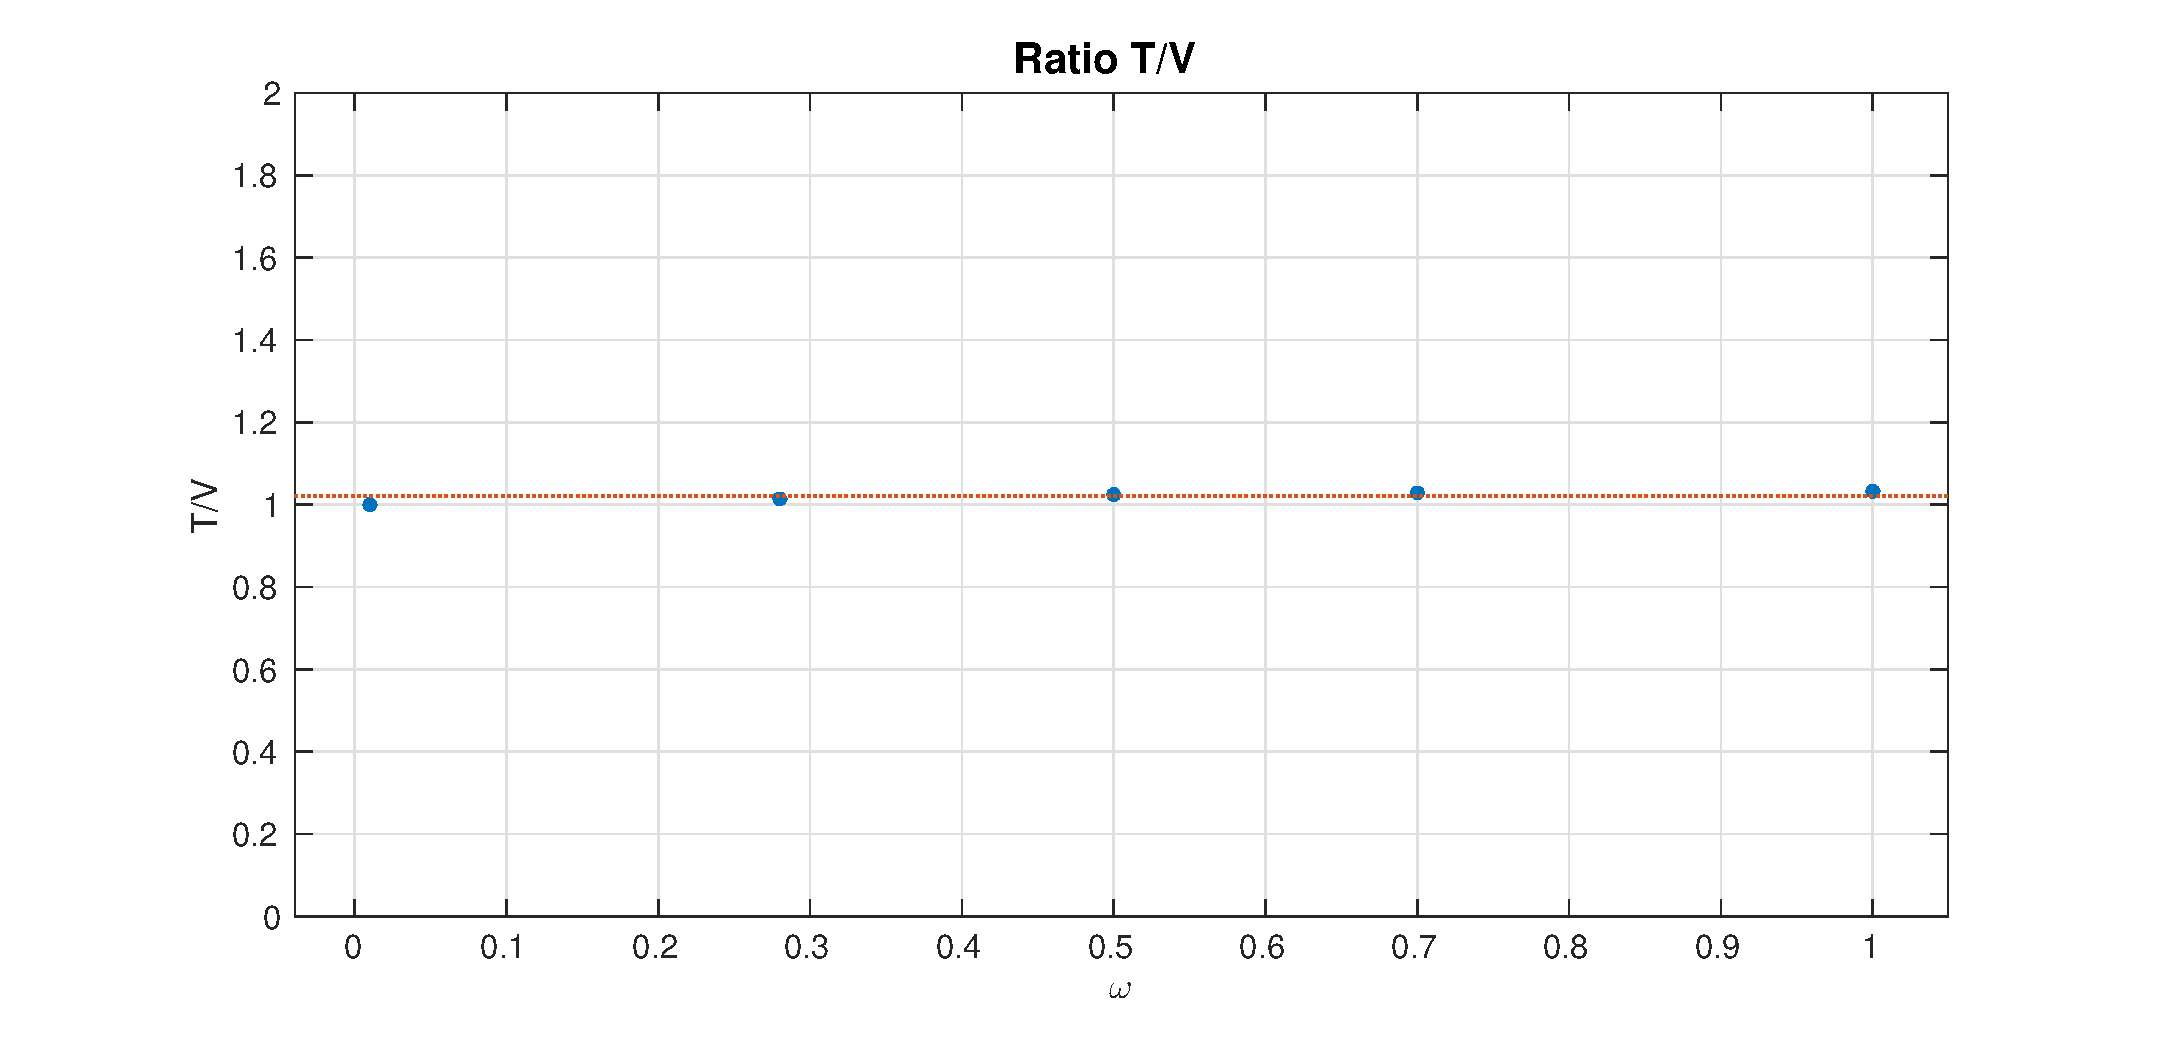
\includegraphics[width=\textwidth]{virial_6e-norep}
	\caption{The ratio $\Braket{T} / \Braket{V}$ for different values of $\omega$ and no electron-electron repulsion. The settings used are: importance sampling with $\Delta t = 0.1$, parallelization (8 threads), $\SI{1e6}{}$ Monte Carlo steps.
	A linear fit gives a ratio of $\SI{1.02 \pm 0.02}{}$, that is still compatible with the expected value $1$.}
	\label{fig:virial_6e-norep}
\end{figure}

\begin{figure}[h]%[H]
	\centering
	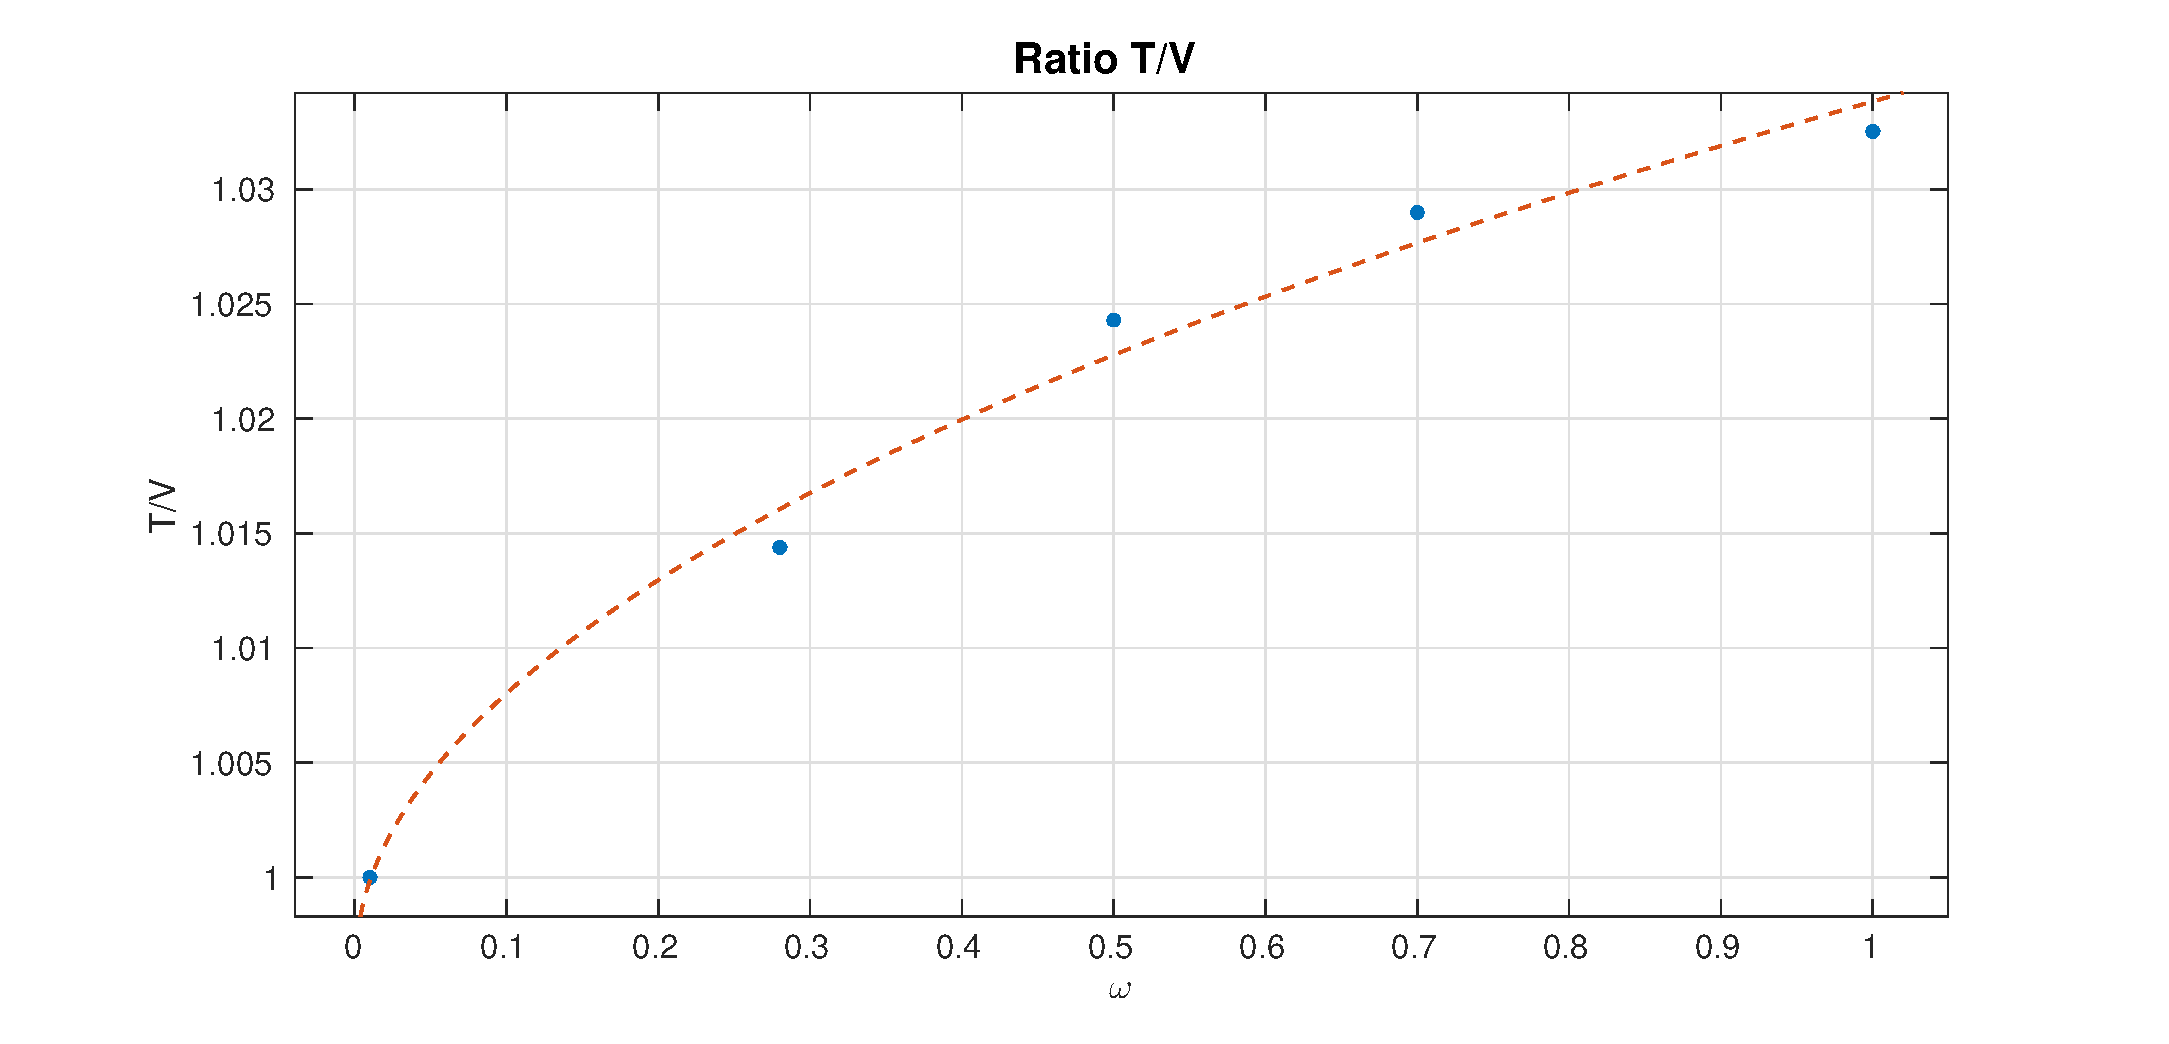
\includegraphics[width=\textwidth]{virial_6e-rep}
	\caption{The ratio $\Braket{T} / \Braket{V}$ for different values of $\omega$ with electron-electron repulsion. The settings used are: importance sampling with $\Delta t = 0.1$, Jastrow factor, parallelization (8 threads), $\SI{1e6}{}$ Monte Carlo steps. The fit is a square root.}
	\label{fig:virial_6e-rep}
\end{figure}

We did again the same calculations (with the same $\omega$ values) for $6$ electrons. This time, we don't obtain a perfect $1$ ratio for the non repulsive case (Figure \ref{fig:virial_6e-norep}); a linear fit gives $\SI{1.02 \pm 0.02}{}$, which is anyway still compatible with the expected value $1$. A possible explanation for this behaviour is that we are not using enough Monte Carlo steps; they are ten times less than the previous case, when we are dealing with a number of electrons that is three times more the 2-electrons case.

The discussion of what we obtain adding the electron-electron repulsion, shown in Figure \ref{fig:virial_6e-rep}, is the same as the 2-electrons case in the previous section. The fit (that \emph{is not} particularly indicative) is of the type
\begin{equation}
	\frac{\Braket{T}}{\Braket{V}} = b\sqrt{c\omega}+d,
\end{equation}
which gives $b = \SI{0.06 \pm 0.01}{}$, $c = \SI{0.416 \pm 0.001}{}$ and $d = \SI{1.00 \pm 0.01}{}$.
%%%%%%%%%%%%%%%%%%%%%%%%%%%%%%%%%%%%%%%%%%%%%%%%%%%%%%%%%%%
%                                                         %
% CHAPTER 06:                                             %
% Analytical derivatives                                  %
%                                                         %
% This file is part of a BSc Thesis Project. See the      %
% LICENSE file for more information about licensing.      %
%                                                         %
% Author:     Matteo Seclì <secli.matteo@gmail.com>       %
% A.Y.:       2014/2015                                   %
% URL:        https://github.com/matteosecli/QMC          %
%                                                         %
%%%%%%%%%%%%%%%%%%%%%%%%%%%%%%%%%%%%%%%%%%%%%%%%%%%%%%%%%%%

\graphicspath{{Mainmatter/figures/PNG/}{Mainmatter/figures/PDF/}{Mainmatter/figures/}}

\chapter{Analytical derivatives}
The most time-consuming part of the Metropolis-Hastings algorithm is the computation of the acceptance ratio, the kinetic energy and the quantum force, that involve the calculation of several first and second derivatives. A way to -- possibly -- improve our program is to use analytical derivatives. Note that this is possible in very few cases -- like this one, so we will take advantage of it.

Let's remember that the wave-function is
\begin{equation}
	\psi_{T} = |\vec{S}^{\uparrow}||\vec{S}^{\downarrow}|J,
\end{equation}
where $|\vec{S}^{\uparrow}|$ is the Slater determinant relative to the spin-up particles, $|\vec{S}^{\downarrow}|$ is the one relative to the spin-down particles and $J$ is the Jastrow factor.

For the quantum force $\vec{F}_i$ relative to particle $i$ we have that
\begin{align}
	\vec{F}_{i} &= 2 \dfrac{1}{\psi_{T}} \nabla_{i} \Psi_{T} \\
	&= 2 \dfrac{\nabla_{i}(|\vec{S}^{\uparrow}||\vec{S}^{\downarrow}|J)}{|\vec{S}^{\uparrow}||\vec{S}^{\downarrow}|J} \\
	&= 2 \left( \dfrac{\nabla_{i}|\vec{S}^{\uparrow}|}{|\vec{S}^{\uparrow}|} + \dfrac{\nabla_{i}|\vec{S}^{\downarrow}|}{|\vec{S}^{\downarrow}|} + \dfrac{\nabla_{i}J}{J} \right).
\end{align}

Since particle $i$ has either spin up or spin down, one of the two terms with the Slater determinant will vanish, because it's not dependant on that particle. So, labelling with $\alpha$ the spin of particle $i$, we have that
\begin{equation}
	\vec{F}_{i} = 2 \left(\dfrac{\nabla_{i}|\vec{S}^{\alpha}|}{|\vec{S}^{\alpha}|} + \dfrac{\nabla_{i}J}{J} \right)
\end{equation}
Doing the same with the local energy, we end up with
\begin{equation}
	E_L= \frac{1}{2} \sum_i \frac{1}{\psi_T} \nabla_i^2 \psi_T + \sum_i V_i
\end{equation}
Then,
\begin{equation}
	\frac{1}{\psi_T} \nabla_i^2 \psi_T= \frac{\nabla_i^2 |\vec{S}^{\alpha}|}{|\vec{S}^{\alpha}|}+\frac{\nabla^2_i J}{J}+2 \frac{\nabla_i |\vec{S}^{\alpha}|}{|
	\vec{S}^{\alpha}|}\frac{\nabla_i J}{J},
	\label{eq:psi_second_derivative}
\end{equation}
where the components relative to the spin opposite to the one of the particle taken into account vanish for the reason explained before.

According to \cite{Hoegberget2013}, the four terms that appear in (\ref{eq:psi_second_derivative}) are
\begin{align}
	\frac{\nabla_i J}{J} 
	&= \sum_{k \neq i=1}^N \frac{a_{ik}}{r_{ik}} \frac{\vec{r}_i-\vec{r}_k}{(1+\beta \, r_{ik})^2} \\
	\frac{\nabla_i^2 J}{J} 
	&= \left|\frac{\nabla_i J}{J} \right|^2+ \sum_{k \neq i=1}^N a_{ik} \frac{(d-3)(\beta \, r_{ik}+1)+2}{r_{ik}(\beta \, r_{ik}+1)^3} \\
	\frac{\nabla_i |\vec{S}|}{|\vec{S}|} 
	&= \sum_k \nabla_i \phi_k (\vec{r}_i^{\text{new}})(\vec{S}_{ki}^{\text{new}})^{-1} \\
	\frac{\nabla_i^2 |\vec{S}|}{|\vec{S}|} 
	&= \sum_k \nabla_i^2 \phi_k (\vec{r}_i^{\text{new}})(\vec{S}_{ki}^{\text{new}})^{-1}
\end{align}
with $k$ that spans the Slater matrix relative to the $i$th particle. The quantities $\nabla_i \phi_k$ and $\nabla^2_i \phi_k$ are also tabulated in \cite{Hoegberget2013}. It's also possible to optimize the determinant of the inverse of the Slater matrix, but we opted here for a numerical computation of the inverse matrix using Armadillo. If one does that, it's also possible to optimize the acceptance ratio to have a even faster code.

\section{Execution times}

Let's see if we have a real gain in speed for the 2-electrons and the 6-electrons cases. Note that we have to run the program with a single thread to avoid extra waiting time on the CPU due to the line
\begin{lstlisting}[language=cpp]
		#pragma omp barrier
\end{lstlisting}
in the parallel cycles. Our benchmarks are shown in Figures \ref{fig:times_2e} and \ref{fig:times_6e}.

\begin{figure}[H]
	\centering
	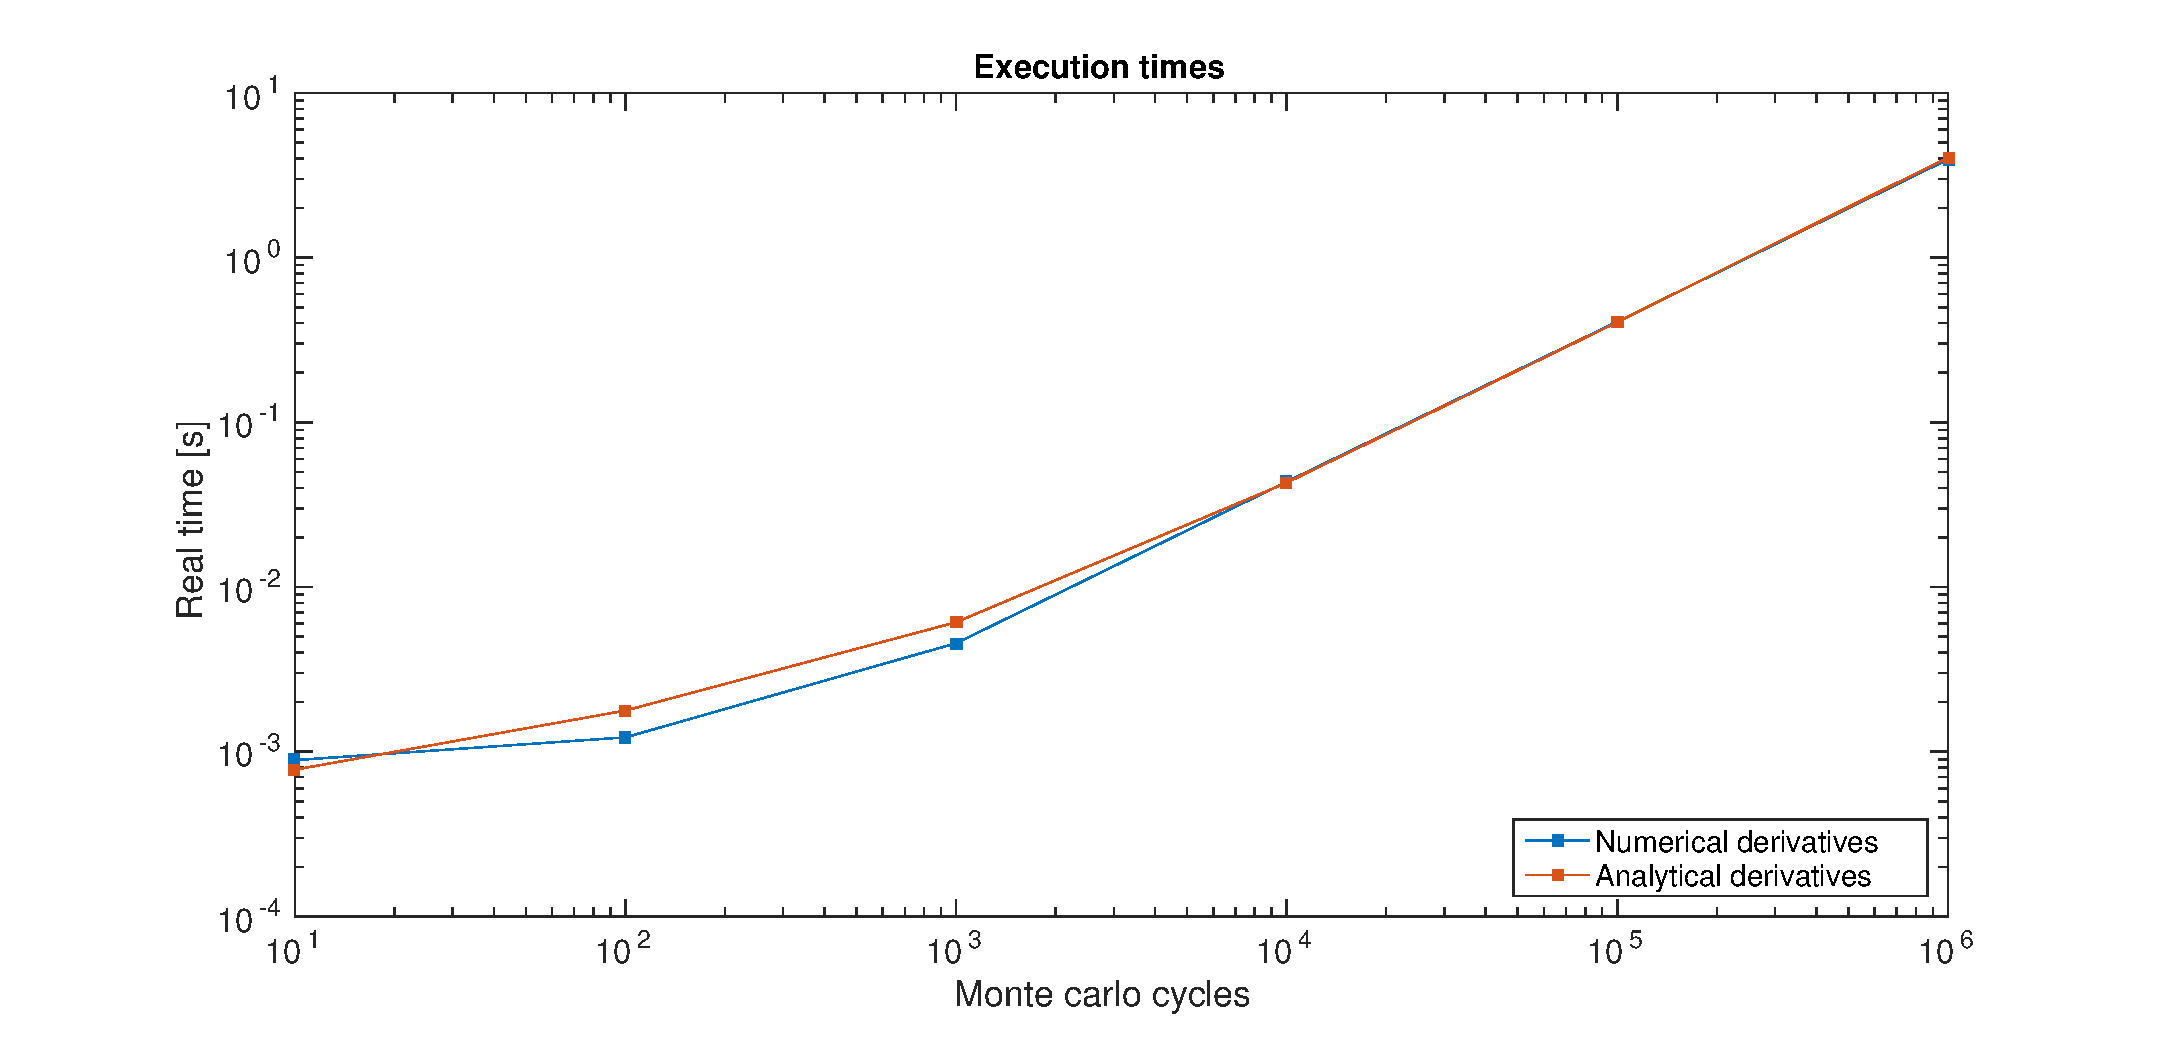
\includegraphics[width=\textwidth]{times_2e}
	\caption{Execution times for 2-electrons and a single pair of variational parameters $(\alpha,\beta)$. The GNU/Linux system tool \texttt{time} was used to take the measurements.}
	\label{fig:times_2e}
\end{figure}

\begin{figure}[H]
	\centering
	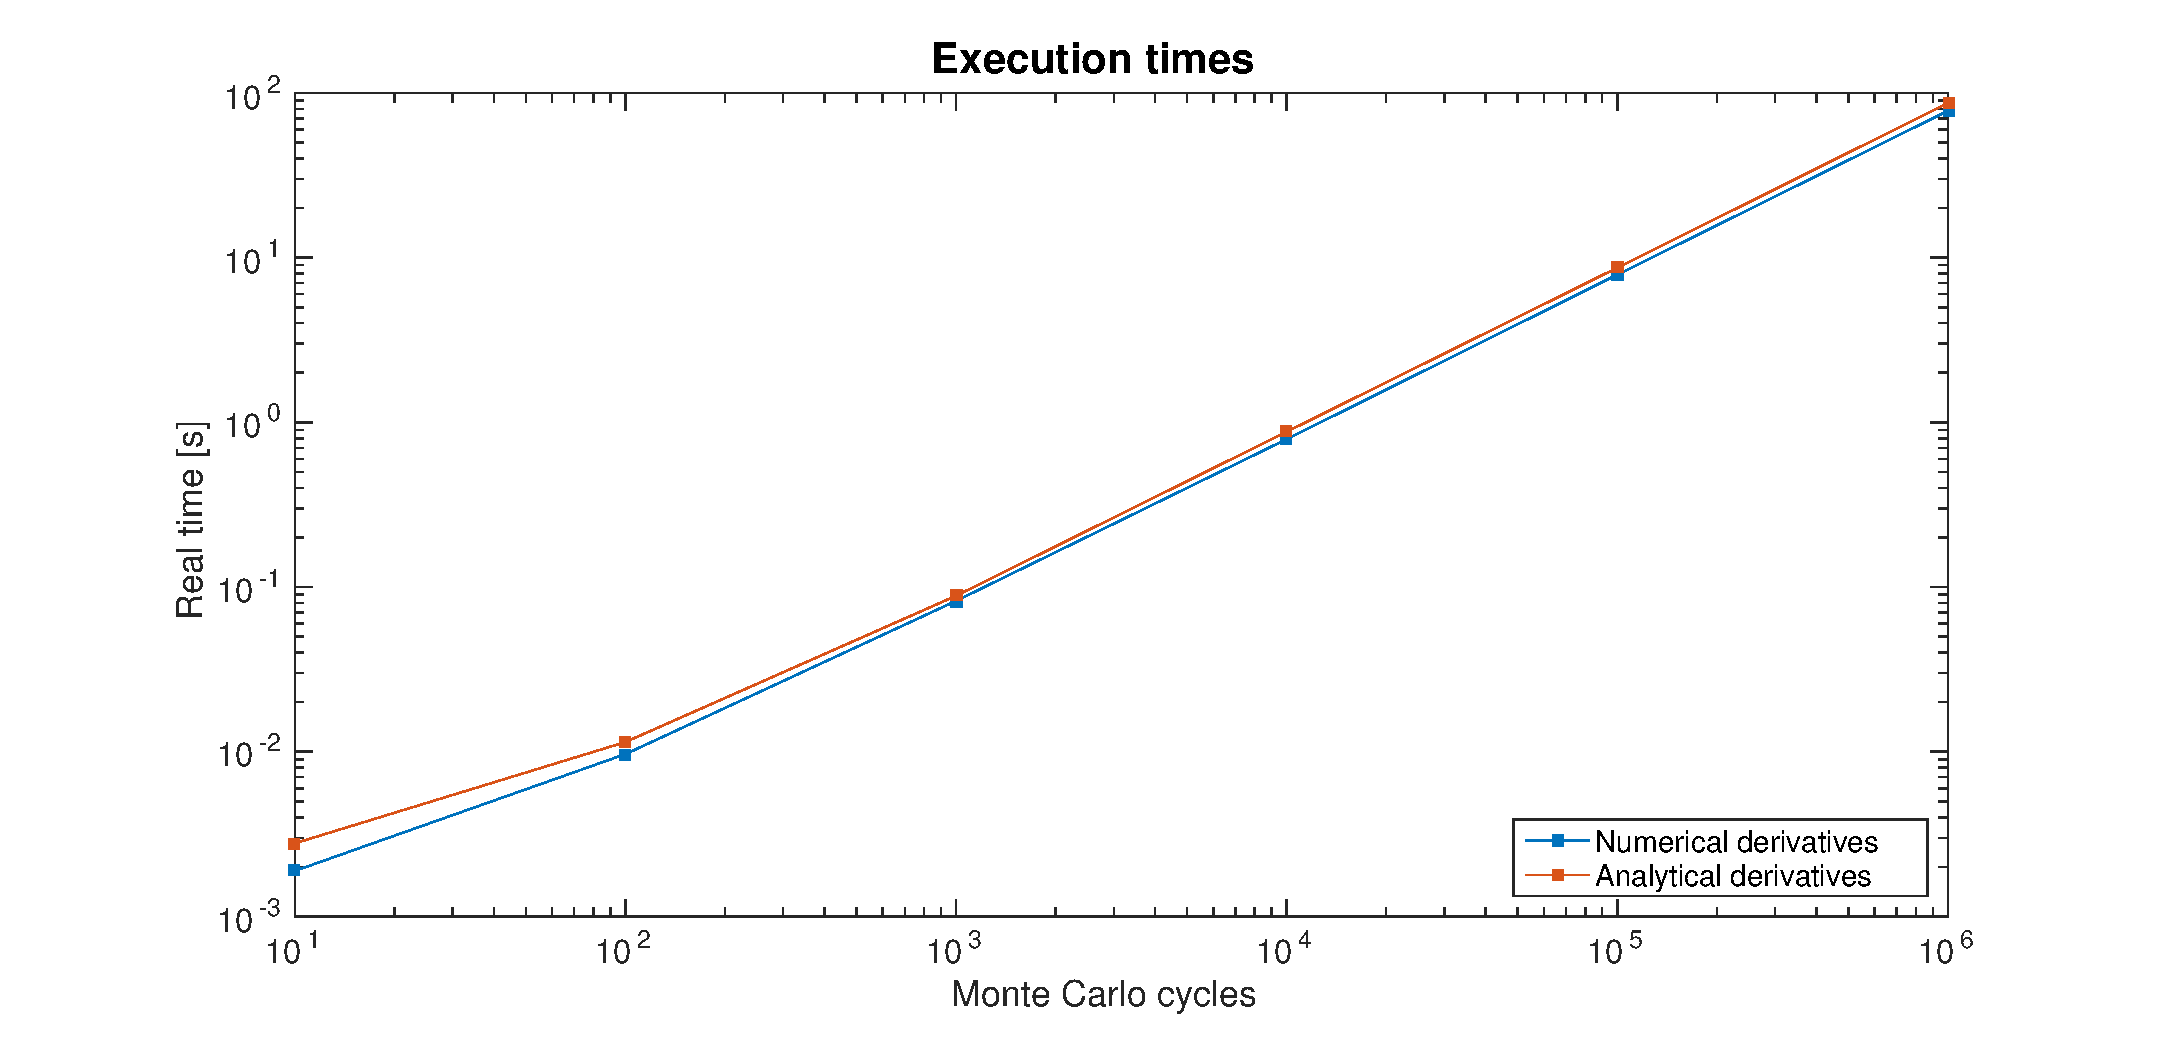
\includegraphics[width=\textwidth]{times_6e}
	\caption{Execution times for 6-electrons and a single pair of variational parameters $(\alpha,\beta)$. The GNU/Linux system tool \texttt{time} was used to take the measurements.}
	\label{fig:times_6e}
\end{figure}

As you see, we don't have great improvements; on the contrary, we obtain a code that is even a little bit slower than the numerical one for the 6-electrons case! However, there are some things that have to be pointed out. First of all we decided to perform a numerical inversion of a matrix, that is really time-consuming (it's a $\mathcal{O}(n^3)$ operation). Secondly there is no optimization of the acceptance ratio, that can be further simplified -- as shown again in \cite{Hoegberget2013}. Lastly, the benefits of numerical derivatives could not appear until one reaches $12$ or even $20$ particles; this is because the computational complexity of a determinant of a matrix is $\mathcal{O}(n^3)$, that for $3 \times 3$ matrices (as the 6-electrons case) is still acceptable. The struggle in calculating big determinants all the time is more evident for higher numbers of particles; for the 12-particles case the Slater determinant is 8 times slower than the 6-particles case, while for the 20-particles case is approximately 37 times slower.

Another thing that has to be noted is that -- with the analytical derivatives -- we obtain slightly lower values for the energy. Deactivating the electron-electron repulsion the discrepancy still persists, meaning that the reason of this fact has to be found in the Slater determinant derivatives implementation. A possible explanation is that we are (numerically) performing the inverse of a matrix that has very small elements, and this could cause a loss of precision.
%%%%%%%%%%%%%%%%%%%%%%%%%%%%%%%%%%%%%%%%%%%%%%%%%%%%%%%%%%%
%                                                         %
% CONCLUSION                                              %
%                                                         %
% This file is part of a BSc Thesis Project. See the      %
% LICENSE file for more information about licensing.      %
%                                                         %
% Author:     Matteo Seclì <secli.matteo@gmail.com>       %
% A.Y.:       2014/2015                                   %
% URL:        https://github.com/matteosecli/QMC          %
%                                                         %
%%%%%%%%%%%%%%%%%%%%%%%%%%%%%%%%%%%%%%%%%%%%%%%%%%%%%%%%%%%

\chapter{Conclusions and perspectives}
I hope that this was an interesting introduction about both quantum dots and the VMC method.

We explored the basic concepts about these devices, but this is just the tip of the iceberg. There are tons of resources about more advanced topics like improved potentials, how to deal with deformation, the effects of a magnetic field, the electronic structure of quantum wires and quantum rings, and so on.

There is an entire world also on the algorithms side. In this project we really showed the power of the VMC method that -- even if it doesn't give automatically the ground state energy of a system -- can be used to approximate it -- to excess -- with a considerable degree of precision. If we have no clues about the properties of the system we can use a brute force sampling, trying to manually set a step-length that gives about an acceptance ratio of $50\%$. But if we are smarter, we can use the information we have about the expected result to implement a more efficient sampling.

This program has been implemented in a highly object-oriented way, following the suggestions contained in \cite{Hoegberget2013}, and can also fully handle the 12-electrons case (look at the implementation of the orbitals in the code). However, it is still \emph{extremely slow} -- practically unusable. So, I'm planning to improve this program using MPI and GPU parallelization, that would give me some extra speed.

I'm also planning to extend this program in such a way that it can handle a custom number of variational parameters, and to improve the trial wave-function with some extra terms as suggested by professor Francesco Pederiva and/or using the Hartree-Fock method. This would require to abandon the analytical derivatives route and concentrate the efforts at improving the algorithm in terms of efficiency.

For me this project has been a springboard into the quantum computational physics world; I enjoyed so much doing this simulation that I've decided to go deeper into this subject and start to explore its full potential in advanced master courses. In particular I want to study improved methods like DMC and DFT, and acquire the theoretical knowledge necessary to fully understand these systems.

I'm also very curious about the world of quantum computation, that is pretty new and still in a dynamic development. It would be interesting to explore how the knowledge I acquired in this project -- once extended in advanced courses as I said -- could be used to develop new concepts and solutions in that field, and vice-versa. I'm planning to take two classes in quantum computation during my master studies, so I hope that I will be able to answer this question very soon -- or at least to start to.

\backmatter
\bibliographystyle{plainnat}
\bibliography{Backmatter/references/ref_database}

\end{document}

%%%%%%%%%%%%%%%%%%%%%%%%%%%%%%%%%%%%%%%%%%%%%%%%%%%%%%%%%%%%%%%%%%%%%%%%%%%%%%%
%                                                                             %
% *** END OF THIS BACHELOR THESIS PROJECT ***                                 %
%                                                                             %
%%%%%%%%%%%%%%%%%%%%%%%%%%%%%%%%%%%%%%%%%%%%%%%%%%%%%%%%%%%%%%%%%%%%%%%%%%%%%%%